\documentclass[DynamicalBook]{subfiles}
\begin{document}
%


\setcounter{chapter}{3}%Just finished 3.

\tableofcontents*

%------------ Chapter ------------%
\chapter{Polynomial functors and dynamics}

\slogan{
The category of polynomial functors is a jackpot. Its beauty flows without bound.}

%-------- Section --------%
\section{Introduction}


In this chapter we will investigate a remarkable category called $\poly$. We will see its intimate relationship with both dynamic processes, data storage and transformations, and decision-making. We will see its intimate relationship with safety and decision-making. But our story begins with something quite humble: middle school algebra.
\begin{align}\label{eqn.polynomial1892}
\yon^\2+\yon+\1 \quad&\quad
\textit{polynomial}
\intertext{
All our polynomials will involve one variable, $\yon$, chosen for reasons we'll explain soon. Polynomials in one variable can be depicted as a set of mini-trees:
}
\label{eqn.poly1892}
\begin{tikzpicture}[trees]
  \node (1) {$\bullet$} 
    child {}
    child {};
  \node[right=.5 of 1] (2) {$\bullet$} 
    child {};
  \node[right=.5 of 2] (3) {$\bullet$};
\end{tikzpicture}
\quad&\quad\textit{arena}
\end{align}
More technically, mini-trees are called \emph{corollas}, so what we're calling an
\emph{arena}, in this chapter, is a set of corollas. 

Intuitively, one might think of each corolla as representing a \emph{decision}. Associated to every decision is a set of \emph{options}. The three decisions we exhibit in \cref{eqn.poly1892} are particularly interesting; they respectively have two options, one option, and no options. Having two options is familiar from life---it's the classic yes/no decision---as well as from Claude Shannon's Information Theory. Having one option is also familiar theoretically and in life: ``sorry, ya just gotta go through it.'' Having no options is when you actually don't get through it: it's ``the end''. While the corollas $\1,\yon,$ and $\yon^\2$ are each interesting as decisions, their sum $\yon^\2+\yon+\1$ has very little theoretical interest; it's just a first example.

In a polynomial like $\4\2\yon^\3+\1\7\yon$, the pure power term $\yon^\3$ has a coefficient of \4\2 next to it, so the corolla with three leaves shows up 42 times%
\footnote{
In standard font, 42 represents the usual natural number. In sans serif font \4\2 represents the set $\4\2=\{1,2,\ldots,42\}$ with 42 elements.
}
in the associated arena. Intuitively, there are 42 situations in which you have a decision with three options. When you put all those decisions together, you have the \emph{arena} associated to $p$. 

Here is a table of terminology. The first column is book-wide terminology, the second is algebraic terminology about polynomials as in \eqref{eqn.polynomial1892}, the third is about the pictures of corollas as in \eqref{eqn.poly1892}, and the fourth column is intuitive terminology.

\begin{equation}\label{eqn.table_terminology}
\small
\begin{tabular}{llll}
\multicolumn{4}{c}{\normalsize Terminology}\\
\textbf{Arena} & \textbf{Polynomial} $p$ & \textbf{Decision Trees} & \textbf{Intuition}\\\hline
Set of positions & $p(\1)$ & Set of roots & Set of situations\\
Interface in position $i$ & Pure power summand $\yon^{p_i}$ & Corolla & Decision\\
Direction $c\in p_i$ & Element of $p_i$ & Leaf & Possibility
\end{tabular}
\end{equation}


\begin{exercise}
Consider the polynomial $p\coloneqq\2\yon^\3+\2\yon+\1$ and the associated arena.
\begin{enumerate}
	\item Draw the arena whose name is $p$ as a set of corollas.
	\item How many roots does this arena have?
	\item How many decisions does this represent?
	\item For each corolla in the arena, say how many leaves it has.
	\item For each decision, how many options does it have?
\end{enumerate}
Now referring instead to the polynomial $q\coloneqq\yon^\nn+\4\yon$:
\begin{enumerate}[resume]
	\item Does the polynomial $q$ have a pure-power summand $\yon^\2$?
	\item Does the polynomial $q$ have a pure-power summand $\yon$?
	\item Does the polynomial $q$ have a pure-power summand $\4\yon$?
	\qedhere
\end{enumerate}

\end{exercise}

\begin{remark}
Though a polynomial is a \emph{functor} and an arena is a \emph{dependent set},
they are so closely related that we do not make a distinction between a
polynomial $p$ and its arena; they are two different syntaxes for the same object. 
\end{remark}

\begin{exercise}
If you were a suitor choosing the arena you love, aesthetically speaking, which would strike your interest? Answer by circling the associated polynomial:
\begin{enumerate}
	\item $\yon^\2+\yon+\1$
	\item $\yon^\2+\3\yon^\2+\3\yon+\1$
	\item $\yon^\2$
	\item $\yon+\1$
	\item $(\nn\yon)^\nn$
	\item $S\yon^S$
	\item $\yon^{\1\0\0}+\yon^\2+\3\yon$
	\item Your poly's name $p$ here.
\end{enumerate}
Any reason for your choice? Draw a sketch of your arena.
\end{exercise}

Before we can really get into this story, let's summarize where we're going: polynomials are going to have really surprising applications to dynamics, data, and decision. Remember, we spoke superlatively of $\poly$ at the beginning of this chapter,
\slogan{
The category of polynomial functors is a jackpot. Its beauty flows without bound}
and we have not yet begun to deliver. So let's introduce some of the applications and mathematics to come.

%---- Subsection ----%
\subsection{Dynamical systems}

Throughout this book, we've seen dynamical systems---machines of various sorts---which have an internal state that can be read out to other systems, as well as updated based on input received from other systems. In the context of this chapter, we'll be looking mainly at deterministic systems, but with a lot of interesting new options:
\begin{enumerate}
	\item The interface of the system can change shape through time.
	\item The wiring diagram connecting a bunch of systems can change in time.
	\item One can speed up the dynamics of a system.
	\item One can introduce ``effects'', i.e.\ as defined by monads on $\smset$.
	\item The dynamical systems on any interface form a topos.
\end{enumerate}

To give some intuition for the first two, imagine yourself as a system, wired up to other systems. You have some input ports: your eyes, your ears, etc., and you have some output ports: your speech, your gestures, etc. And you connect with other systems: your family, your colleagues, the GPS of your phone, etc.
\begin{equation}\label{eqn.wired_forever}
\begin{tikzpicture}[oriented WD, every fit/.style={inner xsep=\bbx, inner ysep=\bby}, bb min width =.5cm, bbx=.5cm, bb port sep =1,bb port length=0, bby=.15cm]
	\node[bb={2}{2}, green!25!black] (X11) {\tiny Alice};
	\node[bb={3}{3}, green!25!black, below right=of X11] (X12) {\tiny you};
	\node[bb={2}{1}, green!25!black, above right=of X12] (X13) {\tiny Bob};
	\node[bb={2}{2}, green!25!black, below right = -1 and 1.5 of X12] (X21) {\tiny GPS};
	\node[bb={1}{2}, green!25!black, above right=-1 and 1 of X21] (X22) {\tiny me};
  \node[bb={2}{2}, fit = {($(X11.north east)+(-1,4)$) (X12) (X13) ($(X21.south)$) ($(X22.east)+(.5,0)$)}, bb name = {\small Wired together like this forever?}] (Z) {};
	\draw (X21_out1) to (X22_in1);
	\draw let \p1=(X22.north east), \p2=(X21.north west), \n1={\y1+\bby}, \n2=\bbportlen in
          (X22_out1) to[in=0] (\x1+\n2,\n1) -- (\x2-\n2,\n1) to[out=180] (X21_in1);
	\draw (X11_out1) to (X13_in1);
	\draw (X11_out2) to (X12_in1);
	\draw (X12_out1) to (X13_in2);
	\draw (Z_in1'|-X11_in2) to (X11_in2);	
	\draw (Z_in2'|-X12_in2) to (X12_in2);
	\draw (X12_out2) to (X21_in2);
	\draw (X21_out2) to (Z_out2'|-X21_out2);
	 \draw let \p1=(X12.south east), \p2=(X12.south west), \n1={\y1-\bby}, \n2=\bbportlen in
	  (X12_out3) to[in=0] (\x1+\n2,\n1) -- (\x2-\n2,\n1) to[out=180] (X12_in3);
	\draw let \p1=(X22.north east), \p2=(X11.north west), \n1={\y2+\bby}, \n2=\bbportlen in
          (X22_out2) to[in=0] (\x1+\n2,\n1) -- (\x2-\n2,\n1) to[out=180] (X11_in1);
	\draw (X13_out1) to (Z_out1'|-X13_out1);
\end{tikzpicture}
\end{equation}
We wrote a little question for you at the top of the diagram. Isn't there something a little funny about wiring diagrams? Maybe for old-fashioned machines, you would wire things together once and they'd stay like that for the life of the machine. But my phone connects to different wifi stations at different times, I drop my connection to Alice for weeks at a time, etc. So wiring diagrams should be able to change in time; $\poly$ will let us do that.

\begin{example}\label{ex.intro_examples_bonds_supplier_assemble}
Here are some familiar circumstances where we see wiring diagrams changing in time.
\begin{enumerate}[itemsep=0pt]
%	\item Airplanes only communicate when they get near enough;
%	\item A phone is connected to 4G or to wifi depending on circumstances;
%	\item A person can choose when to open (receive input through) their eyes and when to speak (produce output);\goodbreak
	\item When too much force is applied to a material, bonds can break;
\end{enumerate}
\[
\begin{tikzpicture}[oriented WD, bb small, bb port length=0]
	\foreach \i in {0,...,4} {
		\node[bb={1}{1}, fill=blue!10] at (1.7*\i,0) (X\i) {};
	}
%	\node[bb={1}{1}, fit=(X0) (X4)] (X) {};
	\foreach \i in {0,...,3} {
		\draw[thick] (X\i_out1) -- (X\the\numexpr\i+1\relax_in1);
	};
	\draw[thick, ->] (X0_in1) -- node[above, font=\tiny] {Force} +(-2.5,0);
	\draw[thick, ->] (X4_out1) -- node[above, font=\tiny] {Force} +(2.5,0) node (R) {};
%
\def\x{21};
	\foreach \i in {0,...,2} {
		\node[bb={1}{1}, fill=blue!10] at (\x+1.7*\i,0) (Y\i) {};
	}
	\foreach \i in {3,...,4} {
		\node[bb={1}{1}, fill=blue!10] at (\x+1.3+1.7*\i,0) (Y\i) {};
	}
%	\node[bb={1}{1}, fit=(Y0) (Y4)] (Y) {};
	\foreach \i in {0,1,3} {
		\draw[thick] (Y\i_out1) -- (Y\the\numexpr\i+1\relax_in1);
	};
	\draw[thick, ->] (Y0_in1) -- node[above, font=\tiny] {Force} +(-2.5,0) node (L) {};
	\draw[thick, ->] (Y4_out1) -- node[above, font=\tiny] {Force} +(2.5,0);
	\node[starburst, draw, minimum width=2cm, minimum height=1.5cm,red,fill=orange,line width=1.5pt] at ($(L)!.5!(R)$)
{Snap!};
\end{tikzpicture}
\]
\begin{quote}
In materials science the Young's modulus accounts for how much force can be transferred across a material as its endpoints are pulled apart. When the material breaks, the two sides can no longer feel evidence of each other. Thinking of pulling as sending a signal (a signal of force), we might say that the ability of internal entities to send signals to each other---the connectivity of the wiring diagram---is being measured by Young's modulus. It will also be visible within $\poly$.
\end{quote}
\begin{enumerate}[resume]
	\item A company may change its supplier at any time;
\end{enumerate}
\begin{equation*}%\label{eqn.supplier}
\begin{tikzpicture}[oriented WD, font=\ttfamily, every node/.style={fill=blue!10}, baseline=(c)]
	\node[bb={0}{1}] (s1) {Supplier 1};
	\node[bb={0}{1}, below=of s1] (s2) {Supplier 2};
	\coordinate (helper) at ($(s1)!.5!(s2)$);
	\node[bb={1}{0}, right=1.5 of helper] (c) {Company};
	\draw (s1_out1) to (c_in1);
	\draw (s2_out1) to +(5pt,0) node[fill=none] {$\bullet$};
\begin{scope}[xshift=3.5in]
	\node[bb={0}{1}] (s1') {Supplier 1};
	\node[bb={0}{1}, below=of s1'] (s2') {Supplier 2};
	\coordinate (helper') at ($(s1')!.5!(s2')$);
	\node[bb={1}{0}, right=1.5 of helper'] (c') {Company};
	\draw (s2'_out1) to (c'_in1);
	\draw (s1'_out1) to +(5pt,0) node[fill=none] {$\bullet$};
\end{scope}
	\node[starburst, draw, minimum width=2cm, minimum height=2cm,align=center,fill=green!10, font=\small, fill=white, line width=1.5pt] at ($(c)!.5!(helper')$)
{Change\\supplier!};
\end{tikzpicture}
\end{equation*}
\begin{quote}
The company can get widgets either from supplier 1 or supplier 2; we could imagine this choice is completely up to the company. The company can decide based on the quality of widgets it has received in the past, i.e.\ when the company gets a bad widget, it updates an internal variable, and sometimes that variable passes a threshold making the company switch states. Whatever its strategy for deciding, we should be able to encode it in $\poly$.
\end{quote}
\begin{enumerate}[resume]
	\item When someone assembles a machine, their own outputs dictate the connection pattern of the machine's components.
\end{enumerate}
\begin{equation*}%\label{eqn.someone}
\begin{tikzpicture}[oriented WD, font=\ttfamily, bb port length=0, every node/.style={fill=blue!10}, baseline=(someone.north)]
	\node[bb port sep=.5, bb={0}{1}] (A) {unit A};
	\node[bb port sep=.5, bb={1}{0}, right=of A] (B) {unit B};
	\coordinate (helper) at ($(A)!.5!(B)$);
	\node[bb={1}{1}, below=2 of helper] (someone) {\tikzsymStrichmaxerl[3]};
	\draw[->, dashed, blue] (someone_in1) to[out=180, in=270] (A.270);
	\draw[->, dashed, blue] (someone_out1) to[out=0, in=270] (B.270);
	\draw (A_out1) -- +(10pt,0);
	\draw (B_in1) -- +(-10pt,0);
%
\begin{scope}[xshift=3.5in]
	\node[bb port sep=.5, bb={0}{1}] (A') {unit A};
	\node[bb port sep=.5, bb={1}{0}, right=.5of A'] (B') {unit B};
	\coordinate (helper') at ($(A')!.5!(B')$);
	\node[bb={1}{1}, below=2 of helper'] (someone') {\tikzsymStrichmaxerl[3]};
	\draw[->, dashed, blue] (someone'_in1) to[out=180, in=270] (A'.270);
	\draw[->, dashed, blue] (someone'_out1) to[out=0, in=270] (B'.270);
	\draw (A'_out1) -- (B'_in1);
\end{scope}
%
	\node[starburst, draw, minimum width=2cm, minimum height=2cm,fill=blue!50,line width=1.5pt, align=center, font=\upshape] at ($(B)!.5!(A')-(0,.6cm)$)
{Attach!};
\end{tikzpicture}
\end{equation*}
\begin{quote}
Have you ever assembled something? Your internal states dictate the connection pattern of some other things. We can say this in $\poly$.
\end{quote}

All of the examples discussed here will be presented in some detail once we have the requisite mathematical theory \cref{ex.bonds_break,ex.supplier_change,ex.assemble_machine}.
\end{example}

\begin{exercise}
Think of another example where systems are sending each other information, but where the sort of information or who it's being sent to or received from can change based on the states of the systems involved. You might have more than two, say $\rr$-many, different wiring patterns in your situation.
\end{exercise}

But there's more that's intuitively wrong or limiting about the picture in \eqref{eqn.wired_forever}. Ever notice how you can change how you interface with the world? Sometimes I close my eyes, which makes that particular way of sending me information inaccessible: that port vanishes and you need to use your words. Sometimes I'm in a tunnel and my phone can't receive GPS. Sometimes I extend my hand to give or receive an object from another person, but sometimes I don't. My ports themselves change in time. Sometimes I even use my output ports to determine the wiring pattern of other machines. We will be able to say all this using $\poly$.

And there's even more that's wrong with the above description. Namely, when I move my eyes, that's actually something you can see---e.g.\ whether I'm looking at you. When I turn around, I see different things, and \emph{you can notice I'm turned around}! When I use my muscles or mouth to express things, my very position changes: my tongue moves, my body moves. So my output is actually achieved by changing position. The model in $\poly$ will be able to express this too.

\begin{example}
Imagine a million little eyeballs, each of which has a tiny brain inside it, all together in a pond of eyeballs. All that an individual eyeball $e$ can do is open and close. When $e$ is open, it can make some distinction about all the rest of the eyeballs in view: maybe it can count how many are open, or maybe it can see whether just one certain eyeball $e'$ is open or closed. But when $e$ is closed, it can't see anything; whatever else is happening, it's all the same to $e$. All it can do in that state is process previous information.

Each eyeball in this system will correspond to the polynomial $\yon^\ord{n}+\yon$, which intuitively consists of two situations, one with $n$-many options, and the other with only one option.

The point is, however, is that the other eyeballs can tell if $e$ is opened or closed. We can imagine some interesting dynamics in this system, e.g.\ waves of openings or closings sweeping over the group, a ripple of openings expanding through the pond.

Talk about real-world applications!
\end{example}

Hopefully you now have an idea of what we mean by mode-dependence: interfaces and wiring diagrams changing in time, based on the states of all the systems involved. We'll see that $\poly$ speaks about mode-dependent systems and wiring diagrams in this sense. 

But $\poly$ is very versatile in its applications. Next we'll show how it relates to information storage and translation.

%---- Subsection ----%
\subsection{Data}

Data is information, maybe thought of as quantized into atomic pieces, but where these atomic pieces are somehow linked together according to a conceptual structure. When a person or organization uses certain data repeatedly, they often find it useful to put their data in a database. This requires organizing the little pieces into a conceptual structure. So when you hear ``database'', just think of it as a conceptual structure filled with examples.

To fix a mental image, let's say that you need to constantly look up employees, what department they're in, who the admin person is for that department, who their manager is, etc. Here's an associated database
\begin{equation}\label{eqn.mytables}
\begin{tabular}{ c | c  c  c}
  \textbf{Employee}&\textbf{FirstName}&\textbf{WorksIn}&\textbf{Mngr}\\\hline
  1&Alan&101&2\\
  2&Ruth&101&2\\
  3&Carla&102&3
\end{tabular}
\hspace{.3in}
\begin{tabular}{ c | c  c}
  \textbf{Department}&\textbf{Name}&\textbf{Admin}\\\hline
  101&Sales&1\\
  102&IT&3\\~
\end{tabular}
%\hspace{.3in}
%\begin{tabular}{ c |}
%	\textbf{String}\\\hline
%	Alan\\
%	IT\\[-3pt]
%	\resizebox{!}{10pt}{$\vdots$}
%\end{tabular}
\end{equation}
We can see it as being associated to the following conceptual scheme, also called a \emph{schema}:
\begin{equation}\label{eqn.myschema}
\cat{C}\coloneqq
\boxCD{white}{
\begin{tikzcd}[row sep=large, ampersand replacement = \&]
 	\LTO{Employee}\ar[rr, shift left, "\text{WorksIn}"]\ar[dr, bend right, "\text{FirstName}"']\ar[loop left, "\text{Mngr}"]\&\&
  \LTO{Department}\ar[ll, shift left, "\text{Admin}"]\ar[dl, bend left, "\text{Name}"]\\
  \&\LTO[\circ]{String}
\end{tikzcd}
\leavevmode\\\bigskip
\text{Department.Admin.WorksIn = Department}
}
\end{equation}
The equation at the bottom says that for any department $d$, if you ask for the admin person and see which department they work in, it's required to be $d$.

What's called $\cat{C}$ in \eqref{eqn.myschema} is a \emph{finitely presented category}, and the database instance presented in \eqref{eqn.mytables} correspond to a functor $I\colon\cat{C}\to\smset$; it sends the object $\text{Employee}\in\cat{C}$ to the set $I(\text{Employee})\coloneqq\{1,2,3\}$. It sends the morphism $\text{Mngr}\colon\text{Employee}\to\text{Employee}$ to the function $I(\text{Mngr})\colon\{1,2,3\}\to\{1,2,3\}$ given by $I(1)=2$, $I(2)=2$, and $I(3)=3$. A functor $\cat{C}\to\smset$ is called a \emph{copresheaf on $\cat{C}$}. So the story of database schemas and their data can be based on the story of categories and their copresheaves.

There's a very important thing that we do with databases: we query them. We ask them questions like ``tell me everyone that's either the admin person of the Math department or their manager''.
\begin{minted}{mysql}
 FOR    d: Department, e: Employee
 WHERE  Name(d)="Math" AND
        (e=Admin(d) OR e=Mngr(Admin(d)))
 RETURN FirstName(e)
\end{minted}
This sort of question is formally called a ``union of conjunctive queries''. We will see this sort of query is intimately connected with $\poly$.

We will also see how databases can be conceived in terms of dynamical systems.

%---- Subsection ----%
\subsection{Decisions}

Consider the following three trees, the first two are infinite (though that's hard to draw):
\[
\begin{tikzpicture}[trees]
\begin{scope}[
  level 1/.style={sibling distance=20mm},
  level 2/.style={sibling distance=10mm},
  level 3/.style={sibling distance=5mm},
  level 4/.style={sibling distance=2.5mm},
  level 5/.style={sibling distance=1.25mm}]
  \node[dgreen] (a) {$\bullet$}
    child {node[dgreen] {$\bullet$}
    	child {node[dgreen] {$\bullet$}
    		child {node[dgreen] {$\bullet$}
  				child {node[dgreen] {$\bullet$}
    				child {}
    				child {}
    			}
  				child {node[dyellow] {$\bullet$}
    				child {}
    				child {}
    			}
  			}
    		child {node[dyellow] {$\bullet$}
					child {node[dgreen] {$\bullet$}
      			child {}
      			child {}
     			}
    			child  {node[red] {$\bullet$}}
  			}
    	}
    	child {node[dyellow] {$\bullet$}
    		child {node[dgreen] {$\bullet$}
  				child {node[dgreen] {$\bullet$}
    				child {}
    				child {}
    			}
  				child {node[dyellow] {$\bullet$}
    				child {}
    				child {}
    			}
  			}
    		child  {node[red] {$\bullet$}}
    	}
    }
    child {node[dyellow] {$\bullet$}
    	child {node[dgreen] {$\bullet$}
    		child {node[dgreen] {$\bullet$}
  				child {node[dgreen] {$\bullet$}
    				child {}
    				child {}
    			}
  				child {node[dyellow] {$\bullet$}
    				child {}
    				child {}
    			}
  			}
    		child {node[dyellow] {$\bullet$}
					child {node[dgreen] {$\bullet$}
      			child {}
      			child {}
     			}
    			child  {node[red] {$\bullet$}}
  			}
  		}
  		child {node[red] {$\bullet$}
  		}
  	}
  ;
\end{scope}
\begin{scope}[
  level 1/.style={sibling distance=13mm},
  level 2/.style={sibling distance=10mm},
  level 3/.style={sibling distance=5mm},
  level 4/.style={sibling distance=2.5mm},
  level 5/.style={sibling distance=1.25mm}]
\node (b) [right=4 of a, dyellow] {$\bullet$}
  child {node[dgreen] {$\bullet$}
  	child {node[dgreen] {$\bullet$}
  		child {node[dgreen] {$\bullet$}
  			child {node[dgreen] {$\bullet$}
    			child {}
    			child {}
   			}
 				child {node[dyellow] {$\bullet$}
   				child {}
   				child {}
   			}
			}
    		child {node[dyellow] {$\bullet$}
					child {node[dgreen] {$\bullet$}
      			child {}
      			child {}
     			}
    			child  {node[red] {$\bullet$}}
  			}
		}
  	child {node[dyellow] {$\bullet$}
  		child {node[dgreen] {$\bullet$}
  			child {node[dgreen] {$\bullet$}
    			child {}
    			child {}
   			}
 				child {node[dyellow] {$\bullet$}
   				child {}
   				child {}
   			}
			}
  		child  {node[red] {$\bullet$}}
  	}
	}
	child {node[red] {$\bullet$}}	
;
\end{scope}
\node (c) [red, right=2 of b] {$\bullet$};
\end{tikzpicture}
\]
These are patterned examples---and we'll understand what this pattern is more clearly in \cref{???}---of what we will call \emph{decision streams}. Decision streams form the objects in a category that also includes the following level-3 abbreviations of binary decision streams (the third of which is a finite stream):
\[
\begin{tikzpicture}[trees]
\begin{scope}[
  level 1/.style={sibling distance=20mm},
  level 2/.style={sibling distance=10mm},
  level 3/.style={sibling distance=5mm},
  level 4/.style={sibling distance=2.5mm}]
  \node (a) {$\bullet$}
    child {node {$\bullet$}
    	child {node {$\bullet$}
    		child {node {$\bullet$}
  			}
    		child {node {$\bullet$}
  				child 
  				child
  			}
    	}
    	child {node {$\bullet$}
  			}
    }
    child {node {$\bullet$}
    	child {node {$\bullet$}
    		child {node {$\bullet$}
  				child
  				child
  			}
    		child {node {$\bullet$}
  				child
  				child
  			}
  		}
  		child {node {$\bullet$}
    		child {node {$\bullet$}
  			}
    		child {node {$\bullet$}
  			}
  		}
  	}
  ;
\end{scope}
\begin{scope}[
  level 1/.style={sibling distance=13mm},
  level 2/.style={sibling distance=10mm},
  level 3/.style={sibling distance=5mm},
  level 4/.style={sibling distance=2.5mm}]
  \node (b) [right=4 of a] {$\bullet$}
    child {node {$\bullet$}
    }
    child {node {$\bullet$}
    	child {node {$\bullet$}
    		child {node {$\bullet$}
  			}
    		child {node {$\bullet$}
  				child
  				child
  			}
  		}
  		child {node {$\bullet$}
    		child {node {$\bullet$}
  				child
  				child
  			}
    		child {node {$\bullet$}
  				child
  				child
  			}
  		}
  	}
  ;
\end{scope}
\begin{scope}[
  level 1/.style={sibling distance=13mm},
  level 2/.style={sibling distance=8mm},
  level 3/.style={sibling distance=5mm},
  level 4/.style={sibling distance=2.5mm}]
  \node (c) [right=4 of b] {$\bullet$}
    child {node {$\bullet$}
    	child {node {$\bullet$}
  		}
  		child {node {$\bullet$}
    		child {node {$\bullet$}
  			}
    		child {node {$\bullet$}
  			}
  		}
    }
    child {node {$\bullet$}
  	}
  ;
\end{scope}
\end{tikzpicture}
\]

The set of such decision streams in fact form the objects of a category with very nice properties (it's a topos), which we call $\sys(\yon^\2+\1)$. The idea is that every corolla in these diagrams has either two options, corresponding to $\yon^\2$, or no options, corresponding to $\1=\yon^\0$.

\begin{exercise}
\begin{enumerate}
	\item Draw a level-3 abbreviation of a decision stream of type $\yon^\2+\yon^\0$.
	\item Draw a level-4 abbreviation of a decision stream of type $\yon$.
	\item Draw a level-3 abbreviation of a decision stream of type $\nn\yon^\2$ by labeling every node with a natural number.
	\qedhere
\end{enumerate}
\end{exercise}

But decisions aren't just about choosing; they're also about trying to accomplish something. The logic of accomplishment is exceptionally rich in this setting. We will concentrate on what we call a \emph{win condition}, which is a subgraph of the decision stream with the property that if $n$ is winning node, then any child of $n$ is also a winning node. 
\[\begin{tikzpicture}[trees,
  level 1/.style={sibling distance=20mm},
  level 2/.style={sibling distance=10mm},
  level 3/.style={sibling distance=5mm},
  level 4/.style={sibling distance=2.5mm}]
  \node (root) {$\bullet$}
    child {node {$\bullet$}
    	child {node {$\bullet$}
    		child {node {$\bullet$}
  			}
    		child {node {$\bullet$}
  				child
  				child
  			}
    	}
    	child {node {$\bullet$}
  			}
    }
    child {node {$\bullet$}
    	child {node {$\bullet$}
    		child {node {$\bullet$}
  				child
  				child
  			}
    		child {node {$\bullet$}
  				child
  				child
  			}
  		}
  		child {node {$\bullet$}
    		child {node {$\bullet$}
  				child
  				child
  			}
    		child {node {$\bullet$}
  			}
  		}
  	}
  ;
 \begin{scope}[every node/.style={circle, inner sep=3pt, blue, draw}]
  \node at (root-1-2)     {};
  \node at (root-2-1-1-1) {};
  \node at (root-2-1-1-2) {};
  \node at (root-2-1-2-1) {};
	\node at (root-2-2) 		{};
  \node at (root-2-2-1) 	{};
  \node at (root-2-2-2) 	{};
  \node at (root-2-2-1-1) {};
  \node at (root-2-2-1-2) {};
 \end{scope}
\end{tikzpicture}
\]
More formally, these are called \emph{sieves}; they form the elements of a logical system called a Heyting algebra: you can take any two sieves and form the intersection or union (which correspond to AND and OR), or even things like implication, negation, and existential and universal quantification. This will give us a calculus of win-conditions for any sort $p$ of decision stream.

%---- Subsection ----%
\subsection{Implementation}

Everything we talk about can actually be implemented in a computer without much difficulty, at least if you have access to a language that supports dependent types. We will continue to use Agda.

What we have been calling polynomials---things like $\yon^\2+\2\yon+\1$---are often called \emph{containers} in the computer science literature. A container consists of a type $S$, usually called the type of \emph{shapes}, and a type $P(s)$ for each term $s:S$, called the type of positions in shape $s$. It's mildly unfortunate that the names clash with our own: for us a container-shape is a position and a container-position is a distinction.

Luckily, the agda code is pretty easy to understand.
\begin{agda}
record Arena : Set where  -- a arena consists of 
   field                       -- two fields
     decn : Set                -- one called decn, a set, and
     posy : pos -> Set         -- one called posy,
                               -- a set that depends on decn
\end{agda}  

%---- Subsection ----%
\subsection{Mathematical theory}\label{subsec.math_theory}

The applications of $\poly$ are quite diverse and interesting, including dynamics, data, and decisions. However it is how the mathematics of $\poly$ supports these applications that is so fantastic. For experts, here are some reasons for the excitement.

\begin{proposition}
$\poly$ is a biCartesian closed category, meaning it has sums, products, and exponential objects. It supports the simply typed lambda calculus.
\end{proposition}

In fact $\poly$ has infinite coproducts, infinite products, and is completely distributive. We'll explain all of this in \cref{??}; for now we continue with the highlights.

\begin{proposition}
Beyond the coCartesian and Cartesian monoidal structures $(\0,+)$ and $(\1,\times)$, the category $\poly$ has two additional monoidal structures, denoted $(\yon,\otimes)$ and $(\yon,\circ)$, which are together duoidal. Moreover $\otimes$ is also a closed monoidal structure and it distributes over $+$.
\end{proposition}

\begin{proposition}
$\poly$ has an adjoint quadruple with $\smset$ and an adjoint pair with $\smset\op$:
\begin{equation*}%\label{eqn.adjoints_galore}
\begin{tikzcd}[column sep=60pt]
  \smset
  	\ar[r, shift left=7pt, "A" description]
		\ar[r, shift left=-21pt, "A\yon"']&
  \poly
  	\ar[l, shift right=21pt, "p(\0)"']
  	\ar[l, shift right=-7pt, "p(\1)" description]
	\ar[l, phantom, "\scriptstyle\Leftarrow"]
	\ar[l, phantom, shift left=14pt, "\scriptstyle\Rightarrow"]
	\ar[l, phantom, shift right=14pt, "\scriptstyle\Rightarrow"]
\end{tikzcd}
\hspace{.6in}
\adjr[50pt]{\smset\op}{\yon^A}{\Gamma p}{\poly}.
\end{equation*}
Each functor is labeled by where it sends $p\in\poly$ or $A\in\smset$.
\end{proposition}

There's a lot we're leaving out of this summary, just so we can hit the highlights.

\begin{proposition}
The functor $\poly\to\smset$ given by $p\mapsto p(\1)$ is a monoidal fibration.
\end{proposition}

In fact it's a monoidal $*$-bifibration in the sense of \cite{shulman2008framed}. But here's where things get really interesting.

\begin{proposition}[Ahman-Uustalu]\label{prop.ahman_uustalu1}
Comonoids in $(\poly,\yon,\circ)$ are categories (up to isomorphism).
\end{proposition}

\begin{proposition}[Niu]
The category $\comon$ has finite coproducts and products, and coproducts in $\comon$ agree with those in $\smcat$.
\end{proposition}

\begin{proposition}
Suppose that the category $\cat{C}$ corresponds under \cref{prop.ahman_uustalu1}, to the comonoid $\com{C}$. Then there is an equivalence of categories
\[
\Cat{Bimod}(\com{C},0)\cong\cat{C}\set
\]
between $(\com{C},0)$-bimodules and $\cat{C}$-copresheaves.
\end{proposition}
We will use the convention that the comonoid $\com{C}$ corresponds to category $\cat{C}$, and similarly for $\com{D}$ and $\cat{D}$, etc. 

\begin{proposition}[Garner]
For any categories $\cat{C}$ and $\cat{D}$, there is an equivalence of categories
\[
\Cat{Bimod}(\com{C},\com{D})\cong\Cat{pra}(\cat{C}\set,\cat{D}\set)
\]
between that of bimodules between comonoids in $\poly$ and parametric right adjoints between copresheaf categories.
\end{proposition}

\begin{proposition}[Niu]
For any category $\cat{C}$ the category of left $\com{C}$-modules is equivalent to the category of functors $\cat{C}\to\poly$,
\[\Cat{Bimod}(\com{C},\yon)\cong\Cat{Fun}(\cat{C},\poly).\]
\end{proposition}

\begin{proposition}
The functor $\comon\to\poly$ has a right adjoint
\[
\adjr{\poly}{\com{K}_-}{u_-}{\comon},
\]
called the \emph{cofree comonoid} construction. It is lax monoidal with respect to $\otimes$.
\end{proposition}

\begin{proposition}
The category $\comon$ has a third symmetric monoidal structure $(\yon,\otimes)$, and the functor $u_-\colon(\comon,\yon,\otimes)\to(\poly,\yon,\otimes)$ is strong monoidal.
\end{proposition}



\begin{proposition}[Niu]\label{prop.sysp_is_topos}
For any polynomial $p$, the category
\[\sys(p)\cong\com{K}_p\set\]
of dynamical systems on $p$ forms a topos.
\end{proposition}

\begin{proposition}\label{prop.poly_map_pregeo_topos}
A morphism $p\to q$ of polynomials induces a pre-geometric morphism between their respective toposes
\[
\adj{\sys(p)}{}{}{\sys(q)}.
\]
\end{proposition}

If you skipped over any of that---or all of that---it'll be no problem whatsoever! We will get to everything in the current section, \ref{subsec.math_theory}, over the next few chapters. To briefly summarize the results we have just seen, they say in particular that there is a full-fledged logic of dynamical systems inhabiting any interface (\cref{prop.sysp_is_topos}), that these logics can be combined and compared (\cref{prop.poly_map_pregeo_topos}), and that the whole story of dynamics carries a strong connection to database theory. There are many avenues for study, but we need to push forward.

Let's begin.


%-------- Section --------%
\section{Introduction to $\poly$ as a category}\label{sec.poly}


In this section, we will set down the basic category-theoretic story of $\poly$, so that we can have a firm foundation from which to speak about dynamical systems, decisions, and data. We begin with the category $\smset$ of sets and functions, and what is arguably the fundamental theorem of category theory, the Yoneda lemma.

%---- Subsection ----%
\subsection{Representable functors and the Yoneda lemma}

\begin{definition}
Given any set $S$, we denote by $\yon^S\colon\smset\to\smset$ the functor that sends any set $X$ to the set $X^S=\smset(S,X)$, and sends any function $h\colon X\to Y$ to the function $h^S\colon X^S\to Y^S$, the one that sends $g\colon S\to X$ to $g\then h\colon S\to Y$.

We refer to $\yon^S$ as the functor \emph{represented by} $S$.
\end{definition}

The symbol $\yon$ stands for Yoneda, for reasons we will get to in \cref{lemma.yoneda}. For now, here are some pictures for your eyes to gaze at; they are the poly's corresponding to various representables:
\begin{equation}\label{eqn.trees_for_gazing}
\begin{tikzpicture}[trees, sibling distance=2mm]
  \node["$\yon^{\5}$" below] (1) {$\bullet$} 
    child foreach \i in {1,...,5}
    ;
\end{tikzpicture}
\qquad
\begin{tikzpicture}[trees, sibling distance=1mm]
  \node["$\yon^{\1\0}$" below] (1) {$\bullet$} 
    child foreach \i in {1,...,10}
    ;
\end{tikzpicture}
\qquad
\begin{tikzpicture}[trees, sibling distance=0.5mm]
  \node["$\yon^{\2\0}$" below] (1) {$\bullet$} 
    child foreach \i in {1,...,20}
    ;
\end{tikzpicture}
\qquad
\begin{tikzpicture}[trees, sibling distance=0.25mm]
  \node["$\yon^{\4\0}$" below] (1) {$\bullet$} 
    child foreach \i in {1,...,40}
    ;
\end{tikzpicture}
\qquad
\begin{tikzpicture}[trees, sibling distance=0.0625mm]
  \node["$\yon^{[0,1]}$" below] (1) {$\bullet$} 
    child foreach \i in {1,...,160}
    ;
\end{tikzpicture}
\end{equation}

\begin{example}
The functor that sends every set $X$ to $X\times X$, and sends $h\colon X\to Y$ to $(h\times h)\colon (X\times X)\to(Y\times Y)$ is representable. 
\end{example}

\begin{exercise}
For each of the following functors $\smset\to\smset$, say if it is representable or not; if it is, say what the representing set is.
\begin{enumerate}
	\item The identity functor $X\mapsto X$.
	\item The constant functor $X\mapsto\2$.
	\item The constant functor $X\mapsto\1$.
	\item The constant functor $X\mapsto\0$.
	\item The functor $X\mapsto X^\nn$.
	\item The functor $X\mapsto 2^X$.
\qedhere
\end{enumerate}
\end{exercise}

\begin{proposition}\label{prop.representable_nt}
For any function $f\colon R\to S$, there is an induced natural transformation $\yon^f\colon\yon^S\to \yon^R$; on any set $X$ the $X$-component $(\yon^f)_X\colon X^S\to X^R$ is given by sending $g\colon S\to X$ to $f\then g\colon R\to X$.
\end{proposition}

\begin{exercise}
Prove that for any function $f\colon R\to S$, what we said was a natural transformation in \cref{prop.representable_nt} really is natural. That is, for any function $h\colon X\to Y$, show that the following diagram commutes:
\[
\begin{tikzcd}
	X^S\ar[r, "h^S"]\ar[d, "X^f"']&
	Y^S\ar[d, "Y^f"]\\
	X^R\ar[r, "h^R"']&
	Y^R\ar[ul, phantom, "?"]
\end{tikzcd}
\qedhere
\]
\end{exercise}

\begin{exercise}
Let $X=\{a,b,c\}$. For each of the following sets $R,S$ and functions $f\colon R\to S$, describe the $X$-component of, i.e.\ the function $X^S\to X^R$ coming from, the natural transformation $\yon^f\colon\yon^S\to\yon^R$.
\begin{enumerate}
	\item $R=\5$, $S=\5$, $f=\id$.
	\item $R=\2$, $S=\1$, $f$ is the unique function.
	\item $R=\1$, $S=\2$, $f(1)=1$.
	\item $R=\1$, $S=\2$, $f(1)=2$.
	\item $R=\0$, $S=\5$, $f$ is the unique function.
	\item $R=\nn$, $S=\nn$, $f(n)=n+1$.
\qedhere
\end{enumerate}
\end{exercise}

\begin{exercise}
Show that the construction in \cref{prop.representable_nt} is functorial
\begin{equation}
\yon^-\colon\smset\op\to\smset^\smset,
\end{equation}
as follows.
\begin{enumerate}
	\item Show that for any set $S$, we have $\yon^{\id_S}\colon\yon^S\to\yon^S$ is the identity.
	\item Show that for any functions $f\colon R\to S$ and $g\colon S\to T$, we have $\yon^g\then\yon^f=\yon^{f\then g}$.
\qedhere
\end{enumerate}
\end{exercise}

\begin{lemma}[Yoneda lemma]\label{lemma.yoneda}
Given a functor $F\colon\smset\to\smset$ and a set $S$, there is an isomorphism
\begin{equation}\label{eqn.yoneda}
F(S)\cong\nat(\yon^S,F)
\end{equation}
where $\nat$ denotes the set of natural transformations. Moreover, \eqref{eqn.yoneda} is natural in both $S$ and $F$.
\end{lemma}
\begin{proof}[Sketch of proof]
For any natural transformation $m\colon\yon^S\to F$, consider the component $m_S\colon S^S\to F(S)$. Applying it to the identity on $S$ as an element of $S^S$, we get an element $m_S(\id_S)\in F(S)$.

For any element $a\in F(S)$, there is a natural transformation $m_a\colon\yon^S\to F$ whose component on $X$ is the function $X^S\to F(X)$ given by sending $g\colon S\to X$ to $F(g)(a)$. In \cref{exc.finish_proof_yoneda} we ask you to show that this is natural in $X$ and that these two constructions are mutually inverse.
\end{proof}

\begin{exercise}\label{exc.finish_proof_yoneda}
Whoever solves this exercise can say they've proved the Yoneda Lemma.
\begin{enumerate}
	\item Show that for any $a\in F(S)$, the maps $X^S\to F(X)$ given as in \cref{lemma.yoneda} are natural in $X$.
	\item Show that the two mappings from \cref{lemma.yoneda} are mutually inverse.
	\item As a corollary of \cref{lemma.yoneda}, show that $\yon^-\colon\smset\op\to\smset^\smset$ is fully faithful, in particular that there is an isomorphism $\nat(\yon^S,\yon^T)\cong S^T$.
\qedhere
\end{enumerate}
\end{exercise}

%---- Subsection ----%
\subsection{Polynomials: sums of representables}

We've seen that for any set $A$, the symbol $\yon^A$ represents a functor $\smset\to\smset$. We will generalize this by adding representable functors together to form polynomials. In some sense the name ``polynomial'' doesn't quite fit, because in algebra polynomials are often taken to be finite sums, whereas we will use sums that may be infinite. However, we are not the first by far to use this term.

So here's the deal. All of our polynomials will be polynomials in one variable, $\yon$; every other letter or number that shows up will represent a set.%
\footnote{For those who clamor for polynomials in many variables, we will see in \cref{??} that the multivariable story falls out of the one-variable story.}
For example, in the following crazy polynomial
\begin{equation}\label{eqn.crazy_poly}
p\coloneqq\rr\yon^\zz+\3\yon^{\3}+A\yon+\sum_{i\in I}Q_i\yon^{R_i+Q_i^2},
\end{equation}
$\rr$ denotes the set of real numbers, $\zz$ denotes the set of integers, $\3$ denotes the set $\{1,2,3\}$, and $A$, $I$, $Q_i$, and $R_i$ denote some arbitrary sets that should have already been defined in order for \eqref{eqn.crazy_poly} to make sense.

The polynomials we already understand at this point are the pure-power polynomials $\yon^A$ for some set $A$; they are representable functors $\yon^A\colon\smset\to\smset.$
So to understand general polynomials like $p$, we just need to understand sums of functors. It will be useful to discuss products of functors at the same time. However, we haven't discussed sums and products of sets yet, so we need to do that first.

\paragraph{Dependent sums and products of sets.}

Let $I$ be a set, and let $X_i$ be a set for each $i\in I$. We denote this
\emph{$I$-indexed collection of sets} --- a \emph{dependent set} ---- by $X\colon I\to\smset$ or more
classically as $(X_i)_{i\in I}$. Choosing one element from one set in the
collection would be denoted $(i,x)$ where $x\in X_i$. Choosing an element from
each set in the collection would give us a function $i \mapsto x_i$ where each
$x_i\in X_i$. This is a sort of function we haven't seen before, at least in
this form --- its codomain \emph{depends} on the element we are applying it to.
Think of a vector field $v$: to each point $p$ it assignes a tangent vector
$v_p$ in the tangent space \emph{at $p$}. We can write the signature of such a
function as
$$f : (i \in I) \to X_i.$$
We call this a \emph{dependent function}, since its codomain depends on the
element of its domain we are applying it to.

\begin{definition}[Dependent sums and products of sets]
Let $I$ be a set and $X\colon I\to\smset$ be an $I$-indexed collection of sets. The sum $\sum_{i\in I}X_i$ (respectively, the \emph{product} $\prod_{i\in I}X_i$) of this collection is the set
\[
\sum_{i\in I}X_i=\{(i,x)\mid i\in I\text{ and }x\in X_i\}
\qqand
\prod_{i\in I}X_i=\{f : (i \in I) \to X_i\}.
\]
\end{definition}

\begin{example}\label{ex.two_sums_and_prods}
If $I=\2=\{1,2\}$ then a collection $X\colon I\to \smset$ is just two sets, say $X_1=\{a,b,c\}$ and $X_2=\{c,d\}$. The sum is the disjoint union
\[\sum_{i\in \2}X_i=X_1+X_2=\{(1,a),(1,b),(1,c),(2,c),(2,d)\}.\]
Its number of elements (cardinality) will always be the sum of the numbers of elements in $X_1$ and $X_2$. Similarly,
\[\prod_{i\in \2}X_i \cong X_1\times X_2=\{(a,c),(a,d),(b,c),(b,d),(c,c),(c,d)\}.\]
\end{example}


\begin{exercise}\label{exc.on_sums_prods_sets}
Let $I$ be a set and let $X_i=\1$ be a one-element set for each $i\in I$. 
\begin{enumerate}
	\item Show that there is an isomorphism of sets $I\cong\sum_{i\in I}\1$.
	\item Show that there is an isomorphism of sets $\1\cong\prod_{i\in I}\1$.
\end{enumerate}
As a special case, suppose $I\coloneqq\varnothing$ and $X\colon \varnothing\to\smset$ is the unique empty collection of sets.
\begin{enumerate}
	\item Is it true that $X_i=\1$ for each $i\in I$?
	\item Show that there is an isomorphism of sets $\0\cong\sum_{i\in\varnothing}X_i$.
	\item Show that there is an isomorphism of sets $\1\cong\prod_{i\in\varnothing}X_i$.
\qedhere
\end{enumerate}
\end{exercise}

\begin{exercise}\label{ex.dependent_product_as_sections}
  Let $X_{(-)} : I \to \smset$ be a set depending on an $i \in I$. There is a
  projection function
  $\pi_1 : \sum_{i \in I} X_i \to I$
  defined by $\pi_1(i, x) = i$.
  \begin{enumerate}
    \item What is the signature of the second projection $\pi_2(i, x) = x$?
      (Hint: its a dependent function).
    \item A \emph{section} of a function $r : A \to B$ is a function $s : B \to
      A$ such that $r \circ s = \id_B$. Show that the dependent product is
      isomorphic to the set of sections of $\pi_1$:
      $$\prod_{i \in I} X_i \cong \{s : I \to \sum_{i \in I} X_i \mid \pi_1
      \circ s = \id_I\}.$$
  \end{enumerate}
\end{exercise}

Where are we, and where are we going? We've define dependent sums and products of sets; that's where we are. Our goal is to define polynomial functors, e.g.\ $\yon^\2+\2\yon+\1$, and the maps between them. Since $\yon^2$, $\yon$, and $\1$ are functors, we just need to define sums of functors $\smset\to\smset$. But we might as well define products of functors at the same time, because they'll very much come in handy.

\paragraph{Dependent sums and products of functors $\smset\to\smset$.}

\begin{definition}[Dependent sums and products of functors $\smset\to\smset$]\label{def.sum_prod}
For any two functors $F,G\colon\smset\to\smset$, let
\[
  (F+G)\colon\smset\to\smset
  \qqand
  (F\times G)\colon\smset\to\smset
\]
denote the functors that respectively assign to each $X\in\smset$ the sets
\[
  (F+G)(X)\coloneqq F(X)+G(X)
  \qqand
	(F\times G)(X)\coloneqq F(X)\times G(X).
\]
More generally, for any set $I$ and functors $(F_i)_{i\in I}$, let
\[
\sum_{i\in I}F_i\coloneq\smset\to\smset
\qqand
\prod_{i\in I}F_i\coloneq\smset\to\smset
\]
denote the functors that respectively assign to each $X\in\smset$ the sum and product of sets
\[
	\Big(\sum_{i\in I}F_i\Big)(X)\coloneqq\sum_{i\in I} F_i(X)
	\qqand
	\Big(\prod_{i\in I}F_i\Big)(X)\coloneqq\prod_{i\in I} F_i(X).
\]
We denote by $\0,\1\colon\smset\to\smset$ the constant functors, which respectively assign $\0$ and $\1$ to each $X\in\smset$.
\end{definition}

\begin{proposition}
Referring to the notation in \cref{def.sum_prod}, the functors $\0$ and $\1$ are respectively an initial object and a terminal object in $\smset^\smset$, the operations $+$ and $\times$ are respectively a binary coproduct and a binary product in $\smset^\smset$, and the operations $\sum_{i\in I}$ and $\prod_{i\in I}$ are arbitrary coproducts and products in $\smset^\smset$.
\end{proposition}
\begin{proof}
By \cref{ex.two_sums_and_prods,exc.on_sums_prods_sets}, it suffices to show that $\sum_{i\in I}F_i$ and $\prod_{i\in I}F_i$ are a sum and product in $\smset^\smset$. This itself is a special case of a more general fact, where sums and products are replaced by arbitrary colimits and limits, and where $\smset^\smset$ is replaced by an arbitrary functor category $\cat{C}^\cat{D}$, where $\cat{C}$ is a category that (like $\smset$) has limits and colimits; see \cite[page 22 -- 23, displays (24) and (25)]{macLane1992sheaves}.
\end{proof}

We've finally arrived: we can define the category of polynomial functors!

\paragraph{$\poly$, the category of polynomial functors}

\begin{definition}[Polynomial functors]
A \emph{polynomial functor} is a functor $p\colon\smset\to\smset$ such that there exists a set $I$, sets $(p_i)_{i\in I}$, and an isomorphism
\[p\cong\sum_{i\in I}\yon^{p_i}\]
to a sum of representables.
A \emph{morphism of polynomial functors} is simply a natural transformation $p\to q$.
\end{definition}

So (up to isomorphism), a polynomial functor is just a sum of representables.

\begin{example}\label{ex.pedantic_poly_eval}
Consider the polynomial $\yon^\2+\2\yon+\1$. It denotes a functor $\smset\to\smset$; what does this functor do to the set $X\coloneqq\{a,b\}$? 
To be very precise and pedantic, let's say
\[
I\coloneqq\4\qqand
  p_1\coloneqq\2,\quad
  p_2\coloneqq\1,\quad
  p_3\coloneqq\1,\quad
  p_4\coloneqq\0\
\]
so that $p\cong\sum_{i\in I}\yon^{p_i}$. Now we have
\[
p(X)\cong
\{(1,a,a),(1,a,b),(1,b,a),(1,b,b),(2,a),(2,b),(3,a),(3,b),(4)\}.
\]
It has $(2^2+2+2+1)$-many, i.e.\ $9$, elements. The representable summand $\yon^A$ throws in all $A$-tuples from $X$, but it's indexed by the name of the summand. In particular if $A=\varnothing$ then it just records the empty tuple at that summand.
\end{example}

\begin{exercise}
In the pedantic style of \cref{ex.pedantic_poly_eval}, write out all the elements of $p(X)$ for $p$ and $X$ as follows:
\begin{enumerate}
	\item $p\coloneqq\yon^\3$ and $X\coloneqq\{4,9\}.$
	\item $p\coloneqq\3\yon^\2+\1$ and $X\coloneqq\{a\}$.
	\item $p\coloneqq\0$ and $X\coloneqq\nn$.
	\item $p\coloneqq\4$ and $X\coloneqq\nn$.
	\item $p\coloneqq\yon$ and $X\coloneqq\nn$.
\qedhere
\end{enumerate}
\end{exercise}

\begin{example}
Suppose $p\coloneqq\yon^\2+\2\yon+1$. As a functor $\smset\to\smset$ it should be able to act not only on sets but on functions. Let $X\coloneqq\{a_1,a_2,b_1\}$, $Y\coloneqq\{a,b,c\}$ and $f\colon X\to Y$ the function sending $a_1,a_2\mapsto a$ and $b_1\mapsto b$. The induced function $p(f)\colon p(X)\to p(Y)$ is shown below
\[
\begin{tikzcd}[row sep=2pt, column sep=3pt, shorten <=-5pt, shorten >=-5pt, dashed]
\LMO{(1,a_1,a_1)}\ar[rrrr, blue, bend left=25pt]&\LMO{(1,a_1,a_2)}\ar[rrr, blue, bend left=25pt]&\LMO{(1,a_1,b_1)}\ar[rrr, blue, bend left=25pt]&[30pt]&
\LMO{(1,a,a)}&\LMO{(1,a,b)}&\LMO{(1,a,c)}&&
\\
\LMO{(1,a_2,a_1)}\ar[rrrru, blue, bend left=10pt]&\LMO{(1,a_2,a_2)}\ar[rrru, blue, bend left=10pt]&\LMO{(1,a_2,b_1)}\ar[rrru, blue, bend left=10pt]&&
\LMO{(1,b,a)}&\LMO{(1,b,b)}&\LMO{(1,b,c)}&&
\\
\LMO{(1,b_1,a_1)}\ar[rrrru, blue, bend left=10pt]&\LMO{(1,b_1,a_2)}\ar[rrru, blue, bend left=10pt]&\LMO{(1,b_1,b_1)}\ar[rrru, blue, bend left=10pt]&&
\LMO{(1,c,a)}&\LMO{(1,c,b)}&\LMO{(1,c,c)}&&
\\
\LMO{(2,a_1)}\ar[rrrr, blue, bend left=25pt]&\LMO{(2,a_2)}\ar[rrr, blue, bend left=25pt]&\LMO{(2,b_1)}\ar[rrr, blue, bend left=25pt]&&
\LMO{(2,a)}&\LMO{(2,b)}&\LMO{(2,c)}&&
\\
\LMO{(3,a_1)}\ar[rrrr, blue, bend left=25pt]&\LMO{(3,a_2)}\ar[rrr, blue, bend left=25pt]&\LMO{(3,b_1)}\ar[rrr, blue, bend left=25pt]&&
\LMO{(3,a)}&\LMO{(3,b)}&\LMO{(3,c)}&&
\\&
\LMO{(4)}\ar[rrrr, blue]&&&&\LMO{(4)}
\end{tikzcd}
\]
\end{example}

\begin{exercise}
Let $p=\yon^\2+\yon$. Choose a function $f\colon\1\to\2$ and write out the induced function $p(f)\colon p(\1)\to p(\2)$.
\end{exercise}

\begin{proposition}\label{prop.apply1}
Let $p\coloneqq\sum_{i\in I}\yon^{p_i}$ be an arbitrary polynomial functor. Then $I\cong p(\1)$, so there is an isomorphism of functors
\begin{equation}\label{eqn.sum_p1}
p\cong\sum_{i\in p(\1)}\yon^{p_i}.
\end{equation}
\end{proposition}
\begin{proof}
We need to show that $I\cong p(\1)$; the latter claim follows directly. In \cref{exc.on_sums_prods_sets} it was shown that $I\cong\sum_{i\in I}\1$, so we just need to show that $(\yon^A)(\1)\cong\1$ for any $A\in\smset$. But $1^A\cong 1$ because there is a unique function $A\to 1$ for any $A$.
\end{proof}

The notation in \eqref{eqn.sum_p1} will be how we denote arbitrary polynomials from now on.

\begin{exercise}\label{exc.apply0}
We saw in \cref{prop.apply1} that for any polynomial $p$, e.g.\ $p=\yon^3+3\yon^2+4$, the set $p(\1)$ gives back the set of summands, in this case $\8$. 

What does $p(\0)$ give you?
\end{exercise}

%---- Subsection ----%
\subsection{Morphisms between polynomial functors are dependent lenses}
\label{subsec.understanding_mor_poly}

For a seasoned category theorist, we've already said enough to calculate the set $\poly(p,q)$ of morphisms between polynomials $p$ and $q$: it's the set of natural transformations between $p$ and $q$, which are sums of representable functors. But it is worth going over this subject at a more leisurely pace, because it helps us insert some intuition that will be very useful later.

In particular, we're going to think about polynomials like $p$ and $q$ using the
intuition from the beginning of the chapter, around the table in
\eqref{eqn.table_terminology}. We said that we'd think of $p$ as a arena: a set
of decisions you can make and what options you have. That is, $p(\1)$ is
conceived as a set of decisions, and for every decision $i\in p(\1)$, we
conceive of the set $p_i$ as the options or \emph{options} available in that
decision. Here's how we write $p$ as an arena:
\[
\begin{tikzcd}
p(\1)\ar[r, "p_-"]&\smset
\end{tikzcd}
\]
Again, every decision $i\in p(\1)$ gets a set $p_i$ of options: that's the whole
content of $p$.
\begin{definition}\label{def.arena_poly}
  An \emph{arena} for the dependent doctrine is a \emph{dependent set} $A^-_{(-)} :
  A^+ \to \smset$; that is, functor from the discrete category on a set $A^+$
  into the category of sets. the set $A^-_{a}$ that each direction $a^-$ lives in
  depends on the position $a \in A^+$. We will write the arena $A^- : A^+ \to
  \smset$ as
  \[\lens{A^-_{a}}{a \in A^+}.\]
\end{definition}

We have just noted that every polynomial $p$ gives an arena $\lens{p_i}{i \in p(\1)}$ whose positions are the decisions in the polynomial and whose directions
are the options.

The maps $f\colon p\to q$ of polynomials are then the ways to \emph{delegate} $p$'s decisions to $q$. Every one of $p$'s decisions, say $i\in p(\1)$, is passed forward to a decision $j\in q(\1)$ for $q$ to make, and every choice $d\in q_j$ that $q$ could make among its options is passed back as some choice $c\in p_i$ among $p$'s options.

\begin{agda}
record Delegation (w : Arena) (w' : Arena) : Set where
   field 
     passfwd : (decn p) -> (decn q)
     passbck : (d : decn p) -> posy q (passfwd d) -> posy p d
\end{agda}

This structure of passing information forward and backwards should look
familiar; its a sort of lens! The difference between this sort of lens and the
sort that we saw in earlier chapters is that the \emph{signature} of the
passback can depend on which decision one is using. We will therefore refer to
these lenses as \emph{dependent lenses}.
\begin{definition}\label{def.dependent_lens}
   A \emph{dependent lens} $\lens{f^{\sharp}}{f} : \lens{A^-_{a}}{a \in A^+}
   \fromto \lens{B^-_{b}}{b \in B^+}$ consists of 
\begin{itemize}
  \item a \emph{passforward} function $f^+ : A^+ \to B^+$, and
\item a dependent \emph{passback} fucntion $f^{\sharp} : (a \in A^+) \to  (
  B^-_{f(a)} \to A^-_{a})$. That is, for every $a \in A^+$, we have a
  passback function $f^{\sharp}(a, -) : B^-_{f(a)} \to A^-_{a}$.
\end{itemize}

The composite of the dependent lens $\lens{f^{\sharp}}{f} : \lens{A^-_{a}}{a \in A^+}
   \fromto \lens{B^-_{b}}{b \in B^+}$ with the dependent lens $\lens{f^{\sharp}}{f} : \lens{B^-_{b}}{b \in B^+}
   \fromto \lens{C^-_{c}}{c \in C^+}$ is given by 
\[
  \lens{g^{\sharp}}{g} \circ \lens{f^{\sharp}}{f} \coloneqq \lens{(a, c^-)
    \mapsto f^{\sharp}(a, g^{\sharp}(f(a), c^-))}{g \circ f}.
\]
This gives us the category of \emph{dependent lenses} $\Cat{DLens}$.
\end{definition}

\begin{proposition}\label{prop.dlens_self_indexing}
Consider the functor $\smset\op\to\smcat$ sending each set $A$ to the slice category $\smset/A$, and sending each $f\colon B\to A$ to the functor $f^*\colon\smset/A\to\smset/B$. Then $\Cat{DLens}$ is equivalent to the category $L$\spiz{notation?} of lenses for this doctrine.
\end{proposition}
\begin{proof}
We define a functor $F\colon \Cat{DLens}\to L$ as follows. An arena $A\coloneqq \lens{A^-_{a}}{a \in A^+}\in\Ob\Cat{DLens}$, assigns a set $A^-_a$ to each $a\in A^+$; let $X\coloneqq\sum_{a\in A^+}A^-_a$ with its obvious map $X\to A^+$. Then $F(A)\coloneqq\lens{X}{A}$ is notation for an object in $L$. We leave it to the reader to give the functor on morphisms, and show that it is fully faithful and essentially surjective.
\end{proof}

\begin{exercise}
Complete the proof of \cref{prop.dlens_self_indexing} as follows.
\begin{enumerate}
	\item To what morphism in $L$ does $F$ assign the morphism $\lens{f^{\sharp}}{f} : \lens{A^-_{a}}{a \in A^+}\fromto \lens{B^-_{b}}{b \in B^+}$?
  \item Show that $F$ is fully faithful.
  \item Show that $F$ is essentially surjective.
 \qedhere 
\end{enumerate}
\end{exercise}

\begin{remark}
Let $p\coloneqq\sum_{i\in p(\1)}\yon^{p_i}$ and $q\coloneqq\sum_{j\in q(\1)}\yon^{q_j}$ be polynomials. We can think of a dependent lens $p\to q$ as in \cref{def.dependent_lens} diagrammatically as follows:
\begin{equation}\label{eqn.colax_poly_map}
\begin{tikzcd}[column sep=small]
	p(\1)\ar[dr, "p_-"']\ar[rr, "f_1"]&~&
	q(\1)\ar[dl, "q_-"]\\&
	\smset\ar[u, phantom, near end, "\overset{f^\sharp}{\Leftarrow}"]
\end{tikzcd}
\end{equation}
That is, $f_1$ is a function (or functor between discrete categories) and $f^\sharp$ is a natural transformation: for each $i\in p(\1)$ with $j\coloneqq f_1(i)$, there is a function $f^\sharp_i\colon q_j\to p_i$.
\end{remark}

Dependent lenses are indeed a generalization of the lenses we saw in \cref{def.lens}.

\begin{proposition}\label{prop.lenses_are_dependent_lenses}
  There is a fully faithful inclusion $\Cat{Lens}_{\smset} \hookrightarrow
  \Cat{DLens}$ interpreting the coKleisli arena $\lens{A^-}{A^+}$ as the \emph{constant}
  dependent arena $\lens{A^-}{a \in A^+}$ (that is, the constant functor $a
  \mapsto A^- : A^+ \to \smset$).
\end{proposition}
\begin{proof}
  We just need to check that the definition of dependent lens specializes
  appropriately to the definition of lens. So, suppose we have constant
  dependent arenas $\lens{A^-}{a \in A^+}$ and $\lens{B^-}{b \in B^+}$. Then a
  dependent lens $\lens{f^{\sharp}}{f} : $
\end{proof}



\begin{lemma}\label{lem.dependent_lens_calculation}
  Using $\sum$s and $\prod$s, we can give a slick definition of dependent lens.
  We have a bijection 
\[\Cat{DLens}\left( \lens{A^-_{a}}{a \in A^+},\, \lens{B^-_{b}}{b \in B^+}
  \right) \cong \prod_{a \in A^+} \sum_{b \in B^+} (A^-_{a})^{(B^-_{b})}\quad\]
\end{lemma}
\begin{proof}
  This is a special case of the upcoming \cref{prop.push_prod_sum_set}, so we'll
  just sketch the proof here. 

  A dependent lens $\lens{f^{\sharp}}{f} : \lens{A^-_{a}}{a \in A^+} \fromto
  \lens{B^-_{b}}{b \in B^+}$ consists of a map $f : A^+ \to B^+$ and a depedent
  map $f^{\sharp} : (a \in A^+) \to (B^-_{f(a)} \to A^-_a)$, while an element of
  the right ahnd side is dependent function
  $$(f, f^{\sharp}) : (a \in A^+) \to \sum_{b \in B^+} (B^-_b \to A^-_a)$$
  which takes an element of $a$ and yields a pair $(f(a), f^{\sharp}(a,-))$.
  These are just two different ways of pairing up the data.
\end{proof}

It seems we are observing that the category of polynomial functors is
equivalent to the category of dependent lenses! Let's state this mathematically and prove it.

\begin{proposition}\label{prop.poly_maps_colax_prod_sum}
Taking a polynomial $p$ to its arena $\lens{p_i}{i \in p(\1)}$ gives
an equivalence between $\poly$ and the category of dependent lenses.

To summarize, we have an isomorphism
\begin{equation}\label{eqn.main_formula}
\poly(p,q)\cong\prod_{i\in p(\1)}\sum_{j\in q(\1)}{p_i}^{q_j} \cong \Cat{DLens}\left( \lens{p_i}{i \in p(\1)},\, \lens{q_j}{j \in q(\1)}\right)
\end{equation}
and composition of polynomial morphisms corresponds to composition of dependent lenses.
\end{proposition}
\begin{proof}
We have an assignment $p \mapsto \lens{p_i}{i \in p(\1)}$ which sends an object
of $\poly$ --- a polynomial functor --- to an object of the category of
dependent lenses --- an arena. We want to show that this object assignment gives
an equivalence of categories. First, we can note that it is surjective up to isomorphism on
objects, since to every arena $\lens{A^-_{a}}{a \in A^+}$ we get the polynomial
functor
\[\sum_{a \in A^+} \yon^{A^-_{a}}\]
and if we take the arena corresponding to the polynomial, we back where we
started since $\sum_{a \in A^+} \1^{A^-_{a}} \cong A^+$.
 
Next, we'll show that the set of natural transformations $\poly(p,q)$ between polynomial functors $p$
and $q$ is isomorphic to the set of dependent lenses between their arenas. We have the following isomorphisms
\begin{align*}
  \poly(p,q)&=
  \nat\Big(\sum_{i\in p(\1)}\yon^{p_i},\;\sum_{j\in q(\1)}\yon^{q_j}\Big)&
  	\text{Definitions}\\&\cong
  \prod_{i\in p(\1)}\nat\Big(\yon^{p_i},\sum_{j\in q(\1)}\yon^{q_j}\Big)&
  	\text{Univ. prop. of coproduct}\\&\cong
  \prod_{i\in p(\1)}\sum_{j\in q(\1)}{p_i}^{q_j}&
  	\text{Yoneda lemma}
\end{align*}
This proves the first part of we called the summary. It says that a morphism
$p\to q$ consists of: for every $i\in p(\1)$ both a choice of $j\in q(\1)$ and a
function from $q_j\to p_i$; the first part determines $f$ (i.e.\ $f(i)=j$) and
the second part just gives $f^\sharp_i$ directly for each $i$.

We can now note that by \cref{lem.dependent_lens_calculation}, $\prod_{i\in
  p(\1)}\sum_{j\in q(\1)}{p_i}^{q_j}$ is isomorphic to the set of dependent
lenses $\lens{p_i}{i \in p(\1)} \fromto \lens{q_j}{j \in q(\1)}$.

Finally, it remains to show that these isomorphisms are functorial. We leave
this to \cref{ex.poly_dependent_lens_functoriality}
\end{proof}

\begin{exercise}\label{ex.poly_dependent_lens_functoriality}
Complete the proof of \cref{prop.poly_maps_colax_prod_sum}.
\end{exercise}

\begin{remark}
The fact in \eqref{eqn.main_formula} that a natural transformation between polynomial functors is
equivalently a dependent lens will be quite important to us; we will call it our
\emph{main formula} for the set of polynomial maps.

In fact, this formula will be so important to us that we will often blur the
difference between a dependent lens $\lens{f^{\sharp}}{f} : \lens{p_i}{i \in
  p(\1)} \fromto \lens{q_j}{j \in q(\1)}$ with the natural transformation $p \to
q$ it corresponds to.
\end{remark}

\begin{example}\label{ex.practice_with_poly_morphisms}
Let $p\coloneqq \yon^\3+\2\yon$ and $q\coloneqq\yon^\4+\yon^\2+\2$
\[
\begin{tikzpicture}[rounded corners]
	\node (p1) [draw, blue!50!black, "$p$" above] {
	\begin{tikzpicture}[trees, sibling distance=2.5mm]
    \node["\tiny 1" below] (1) {$\bullet$} 
      child {}
      child {}
      child {};
    \node[right=.5 of 1,"\tiny 2" below] (2) {$\bullet$} 
      child {};
    \node[right=.5 of 2,"\tiny 3" below] (3) {$\bullet$}
      child {};
  \end{tikzpicture}
  };
%
	\node (p2) [draw, red!50!black, right=2 of p1, "$q$" above] {
	\begin{tikzpicture}[trees, sibling distance=2.5mm]
    \node["\tiny 1" below] (1) {$\bullet$} 
      child {}
      child {}
      child {}
      child {};
    \node[right=.5 of 1,"\tiny 2" below] (2) {$\bullet$} 
      child {}
      child {};
    \node[right=.5 of 2,"\tiny 3" below] (3) {$\bullet$}
    ;
    \node[right=.5 of 3,"\tiny 4" below] (4) {$\bullet$}
    ;
  \end{tikzpicture}
  };
\end{tikzpicture}
\]
To give a dependent lens $p\to q$, one delegates each $p$-decision $i\in p(\1)$ to a $q$-decision $j\in q(\1)$, and then each option in $q_j$ is passed back to one in $p_i$.

How many ways are there to do this? Before answering this, let's just pick one.
\[
\begin{tikzpicture}
	\node (p1) {
	\begin{tikzpicture}[trees, sibling distance=2.5mm]
    \node[blue!50!black, "\tiny 1" below] (1) {$\bullet$} 
      child {coordinate (11)}
      child {coordinate (12)}
      child {coordinate (13)};
    \node[right=1.5 of 1, red!50!black, "\tiny 1" below] (2) {$\bullet$} 
      child {coordinate (21)}
      child {coordinate (22)}
      child {coordinate (23)}
      child {coordinate (24)};
    \draw[|->, shorten <= 3pt, shorten >= 3pt] (1) -- (2);
    \begin{scope}[densely dotted, bend right, decoration={markings, mark=at position 0.75 with \arrow{stealth}}]
      \draw[postaction={decorate}] (21) to (13);
      \draw[postaction={decorate}] (22) to (11);
      \draw[postaction={decorate}] (23) to (13);
      \draw[postaction={decorate}] (24) to (13);
    \end{scope}
  \end{tikzpicture}	
	};	
%
	\node (p2) [right=1 of p1] {
	\begin{tikzpicture}[trees, sibling distance=2.5mm]
    \node[blue!50!black, "\tiny 2" below] (1) {$\bullet$} 
      child {coordinate (11)};
    \node[right=of 1, red!50!black, "\tiny 1" below] (2) {$\bullet$} 
      child {coordinate (21)}
      child {coordinate (22)}
      child {coordinate (23)}
      child {coordinate (24)};
    \draw[|->, shorten <= 3pt, shorten >= 3pt] (1) -- (2);
    \begin{scope}[densely dotted, bend right, decoration={markings, mark=at position 0.75 with \arrow{stealth}}]
      \draw[postaction={decorate}] (21) to (11);
      \draw[postaction={decorate}] (22) to (11);
      \draw[postaction={decorate}] (23) to (11);
      \draw[postaction={decorate}] (24) to (11);
    \end{scope}
  \end{tikzpicture}	
	};	
%
	\node (p3) [below right=-1.05cm and 1 of p2] {
	\begin{tikzpicture}[trees, sibling distance=2.5mm]
    \node[blue!50!black, "\tiny 3" below] (1) {$\bullet$} 
      child {};
    \node[right=of 1, red!50!black, "\tiny 4" below] (2) {$\bullet$} 
		;
    \draw[|->, shorten <= 3pt, shorten >= 3pt] (1) -- (2);
  \end{tikzpicture}	
	};	
\end{tikzpicture}
\]
This represents one morphism $p\to q$.

So how many different morphisms are there from $p$ to $q$? One way to figure it out is to use the formula \eqref{eqn.main_formula}, but that might need some explaining; we go through such notation in an interlude after \cref{exc.practice_poly_maps}. For now, we can just count ``pre-theoretically''.

The first $p$-decision can be delegated to $q$-decision 1, 2, 3, or 4. Delegating it to the first $q$-decision requires choosing how each of the four options $(q_1=\4)$ are to be assigned one of $p_1=\3$ options; there are $3^4$ ways to do this. Similarly, we can calculate all the ways to delegate the first $p$-decision: there are $3^4+3^2+3^0+3^0=92$. 

The second $p$-decision can be delegated to $q$-decision 1, 2, 3, or 4. There are $1^4+1^2+1^0+1^0=4$ ways to do this; similarly there are four ways to delegate the third $p$-decision to a $q$-decision.

In total, there are $92*4*4=1472$ morphisms $p\to q$, just twenty less than the number of years between Jesus's famous year and Columbus's famous year. Coincidence? 
\end{example}

\begin{exercise}\label{exc.practice_poly_maps}
\begin{enumerate}
	\item Draw the poly's (unions of corollas as in \cref{eqn.poly1892}) associated to $p\coloneqq\yon^3+\yon+1$, $q\coloneqq \yon^2+\yon^2+2$, and $r\coloneqq\yon^3$.
	\item Give an example of a morphism $p\to q$ and draw it as we did in \cref{ex.practice_with_poly_morphisms}.
	\item Explain your morphism as a ``delegation'' in the sense of \cref{subsec.understanding_mor_poly}.
	\item Explain in those terms why there can't be any morphisms $p\to r$.
\qedhere
\end{enumerate}
\end{exercise}

\begin{exercise}
For any polynomial $p$ and set $A$, e.g.\ $A=\2$, the Yoneda lemma gives an isomorphism $p(A)\cong \poly(\yon^A,p)$.
\begin{enumerate}
	\item Choose a polynomial $p$ and draw the associated poly as well as $\yon^\2$.
	\item Count all the maps $\yon^2\to p$.
	\item Is it equal to $p(\2)$?
\qedhere
\end{enumerate}
\end{exercise}

\paragraph{Working with $\sum$ and $\prod$ formulas.}
Here's how to understand and work with a set that involves $\sum$'s and $\prod$'s, e.g.\ something like
\begin{equation}\label{eqn.misc98339}
\sum_{i\in I}\prod_{j\in J(i)}\sum_{k\in K(i,j)}X(i,j,k).
\end{equation}
To understand it, you ask ``what is involved in choosing an element of this set?'' 

The answer given by the formula \eqref{eqn.misc98339} begins by saying ``To choose an element of \eqref{eqn.misc98339}, first..." and then you begin pronouncing the formula. Every time you see $\sum_{i\in I}...$, say ``choose an element $i\in I$; then, ...''. Every time you see $\prod_{j\in J}$, say ``for each $j\in J$, ...''. At the very end when you see some $X$, say ``conclude by choosing an element of $X$''.

So the formula in \eqref{eqn.misc98339} would be pronounced as follows:
\begin{quote}
To choose an element of \eqref{eqn.misc98339}, first choose an element $i\in I$. Then, for every $j\in J(i)$, choose an element $k\in K(i,j)$; then, conclude by choosing an element of $X(i,j,k)$.
\end{quote}
Note that the choice of $k\in k(i,j)$ can depend on $i$ and $j$; it must be able to because these sets $K(i,j)$ can be different for different $i,j$.

\begin{example}[Notation for $\sum\prod$ stuff]\label{ex.notation_sum_prod}
Here we give notation for the elements of a set involving $\sum$'s and $\prod$'s such as that in \eqref{eqn.misc98339}.

Let $I=\{1,2\}$, let $J(1)=\{j\}$ and $J(2)\coloneqq\{j,j'\}$, let $K(1,j)\coloneqq\{k_1,k_2\}$, $K(2,j)\coloneqq\{k_1\}$, and $K(2,j')\coloneqq\{k'\}$, and let $X(i,j,k)=\{x,y\}$ for all $i,j,k$. Now the formula 
\[\sum_{i\in I}\prod_{j\in J(i)}\sum_{k\in K(i,j)}X(i,j,k)\]
 has been given meaning as an actual set. Here is a list of all eight of its elements:
\[
\left\{
\begin{gathered}
	\big(1, j\mapsto(k_1,x)\big),\qquad
	\big(1, j\mapsto(k_1,y)\big),\qquad
	\big(1, j\mapsto(k_2,x)\big),\qquad
	\big(1, j\mapsto(k_2,y)\big),\\
	\big(2, j\mapsto(k_1,x), j'\mapsto(k_1,x)\big),\qquad
	\big(2, j\mapsto(k_1,x), j'\mapsto(k_1,x)\big),\\
	\big(2, j\mapsto(k_1,x), j'\mapsto(k_1,x)\big),\qquad
	\big(2, j\mapsto(k_1,x), j'\mapsto(k_1,x)\big)
\end{gathered}
\right\}
\]
In each case, we first chose an element $i\in I$, either 1 or 2. Then for each $j\in J(i)$ we chose an element $k\in K(i,j)$; then we concluded by choosing an element of $X(i,j,k)$.
\end{example}

\begin{exercise}
With $I$, $J$, $K$, and $X$ as in \cref{ex.notation_sum_prod}, consider the set
\[\prod_{i\in I}\sum_{j\in J(i)}\prod_{k\in K(i,j)}X(i,j,k).\]
\begin{enumerate}
	\item Pronounce it using the ``To choose an element'' formulation just below \eqref{eqn.misc98339}.
	\item How many elements are in it?
	\item Write out three of them in the style of \cref{ex.notation_sum_prod}.
\qedhere
\end{enumerate}
\end{exercise}

The following is sometimes called the \emph{type-theoretic axiom of choice} or the \emph{completely distributive property}, in this case of $\smset$. It is almost trivial, once you understand what it's saying; for example once the statement is written in agda, its proof is one short line of agda code. 

\begin{proposition}[Pushing $\prod$ past $\sum$]\label{prop.push_prod_sum_set}
For any set $I$, collection of sets $\{J(i)\}_{i\in I}$, and collection of sets $\{X(i,j)\}_{i\in i, j\in J(i)}$, we have a bijection
\begin{equation}\label{eqn.set_completely_distributive}
\sum_{j\in \prod_{i\in I}J(i)}\;\prod_{i\in I}X(i,j(i))
\cong
\prod_{i\in I}\sum_{j\in J(i)}X(i,j).
\end{equation}
\end{proposition}
\begin{proof}
We'll do this the old-fashioned way: by giving a map from left to right, and a
map from right to left, and showing that they are mutually inverse. 

First, let's go from left to right. An element of the set on the left is a pair
of a function $j \in \prod_{i \in I}J(i)$ together with a function $f \in
\prod_{i \in I} X(i, j(i))$. We then get an element of the set on the right as follows:
\[i \mapsto (j(i), f(i)).\]

Now, let's go right to left. An element of the set on the right is a function $f
\in \prod_{i \in I} \sum_{j \in J(i)} X(i, j)$. We can then form the following
pair in the left hand set:
\[((i \mapsto \pi_1f(i)), (i \mapsto \pi_2f(i)))\]
where $\pi_1f(i)$ is the first component of the pair $f(i)$ and $\pi_2f(i)$
is the second component.

Now, we just need to check that a round trip takes us back where we were. If we
start on the left, our round trip gives us the pair
\[((i \mapsto \pi_1(j(i), f(i))), (i \mapsto \pi_2(j(i), f(i)))).\]
But $\pi_1(j(i), f(i)) = j(i)$ and $\pi_2(j(i), f(i)) = f(i)$ by definition, so
we're back where we started. On the other hand, starting on the right gives us
the function
\[i \mapsto (\pi_1f(i), \pi_2f(i)).\]
But again, since $f(i)$ is the pairing of its components $\pi_1(f(i))$ and
$\pi_2(f(i))$, we're back where we started.

\erase{
We start with the function from left to right. To give such a function it suffices by the universal property of products and coproducts to fix an arbitrary $j_0\in\prod_{i\in I}J(i)$ and $i_0\in I$, and provide a function $\prod_{i\in I}X(i,j_0(i))\to\sum_{j\in J(i_0)}X(i_0,j)$. We do so by first projecting onto the $i_0$ factor and then including into the $j_0(i_0)$ summand
\[
  \prod_{i\in I}X(i,j_0(i))\to 
  X(i_0,j_0(i_0))\to
  \sum_{j\in J(i_0)}X(i_0,j).
\]
We have now given the function from left to right. To go the other way..
}
\end{proof}

\begin{exercise}\label{ex.dependent_lens_calculation}
  Use \cref{prop.push_prod_sum_set} to give another proof of
  \cref{lem.dependent_lens_calculation}. (Hint: express the left hand side as a
  dependent sum.)
\end{exercise}

Below, e.g.\ in \cref{exc.practice_sum_prod}, you'll often see alternating sums and products; using \cref{eqn.set_completely_distributive}, you can always put it into sums-then-products (``disjunctive normal'') form.

When $J(i)=J$ does not depend on $i\in I$, the formula in \eqref{eqn.set_completely_distributive} is much easier:
\[
\prod_{i\in I}\sum_{j\in J}X(i,j)\cong\sum_{j\colon I\to J}\;\prod_{i\in I}X(i,j).
\]

\begin{exercise}\label{exc.practice_sum_prod}
Let $p,q$ be polynomials as in \cref{prop.poly_maps_colax_prod_sum}. Recall from
our main formula \eqref{eqn.main_formula} that there is an isomorphism between polynomia$\poly(p,q)\cong\prod_{i\in p(\1)}\sum_{j\in q(\1)}{p_i}^{q_j}.$ 
\begin{enumerate}
\item Is it true that the following are isomorphic?
\[
  \poly(p,q)
  \cong^?
  \prod_{i\in p(\1)}\sum_{j\in q(\1)}\prod_{d\in q_j}\sum_{c\in p_i}\1
\]
\item Is it true that there is an isomorphism
	\begin{equation}\label{eqn.useful_misc472}
	\poly(p,q)\cong^?\sum_{f_1\colon p(\1)\to q(\1)}\prod_{j\in q(\1)}\smset\Big(q_j,\prod_{\{i\in p(\1)\mid f_1(i)= j\}}p_i\Big).
	\end{equation}
\item If the answer to \#2 is ``yes'', then say how any element of the right-hand side gives a way of delegating decisions from $p$ to $q$. If ``no'', give intuition for why the two sets are not isomorphic.
\qedhere
\end{enumerate}
\end{exercise}


\paragraph{Back to maps of polynomials}
After that interlude, you are hopefully more comfortable with our main formula
\cref{eqn.main_formula} describing the set of morphisms between two arbitrary
polynomial functors as dependent lenss. Let's practice.

\begin{example}[Constants are sent to constants]\label{ex.const_to_const}
Any natural transformation $p\to q$ must send constants in $p$ to constants in $q$. So if $p$ has constant terms and $q$ doesn't, e.g.\ if $p=\yon^\2+\1$ and $q=\yon^3$, then there are no maps $p\to q$. 

Indeed, let's more generally say $p\coloneqq\sum_{i\in p(\1)}\yon^{p_i}$ and
$q\coloneqq\sum_{j\in q(\1)}\yon^{q_j}$ are polynomials, and that we have a map
$p\to q$ corresponding to a dependent lens $\lens{p_i}{i \in p(\1)} \fromto
\lens{q_j}{j \in q(\1)}$. If there is some $i_0\in p(\1)$ such that $p_{i_0}=\0$, then the formula says that for $i_0$ our map has chosen a $j\in q(1)$ and a function $q_j\to p_i$. But in order for such a function to exist, if $p_i$ is empty, $q_j$ must be too.
\end{example}

\begin{exercise}
For each of the following $p,q$, count the number of natural transformations $p\to q$:
\begin{enumerate}
	\item $p=\yon^3$,\quad $q=\yon^4$.
	\item $p=\yon^3+1$,\quad $q=\yon^4$.
	\item $p=\yon^3+1$,\quad $q=\yon^4+1$.
	\item $p=4\yon^3+3\yon^2+\yon$,\quad $q=\yon$.
	\item $p=4\yon^3$,\quad $q=3\yon$.
\qedhere
\end{enumerate}
\end{exercise}

%---- Subsection ----%
\subsection{Prepare for dynamics}\label{subsec_prepare_dyn}

As beautiful as the category $\poly$ is---and to be clear we have not really begun to say what is so special about it---discussing its virtues is not our goal. We want to use it!

Polynomial functors are a setting in which to speak about dynamics, data, and decision. We want the reader to understand this deeply as they go through the mathematics. So in order to make the story a bit more seamless, we discuss a few relevant aspects of $\poly$ that we can use immediately.


\paragraph{Finite products}
The category $\poly$ has limits and colimits, is Cartesian closed, has epi-mono factorizations, is completely distributive, etc., etc. However, in order to tell a good story of dynamics, we only need finite products right now. These will be useful for letting many different interfaces control the same internal dynamics.

\begin{proposition}\label{prop.poly_times}
The category $\poly$ has finite products. 
\end{proposition}
\begin{proof}
We will see that $\1$ is a terminal object and that the product of $p$ and $q$ in $\poly$ is the usual product of $p$ and $q$ as polynomials. That is, if $p\coloneqq\sum_{i\in p(\1)}\yon^{p_i}$ and $q\coloneqq\sum_{i\in q(\1)}\yon^{q_i}$ are in standard notation, then
\begin{equation}\label{eqn.poly_times}
p\times q\cong\sum_{i\in p(\1)}\sum_{j\in q(\1)}\yon^{p_i+q_j}.
\end{equation}
We leave the proof as an exercise; see \cref{exc.poly_times}.
\end{proof}

\begin{exercise}\label{exc.poly_times}
Use \cref{eqn.main_formula} to prove \cref{prop.poly_times} using dependent lenses. In particular:
\begin{enumerate}
	\item Prove that $\1$ is terminal in $\poly$.
	\item Prove that for polynomials $p,q$, their product is given by the formula in \eqref{eqn.poly_times}.
\qedhere
\end{enumerate}
\end{exercise}

We will begin writing $pq$ rather than $p\times q$:
\begin{equation} \tag{Notation}
pq\coloneqq p\times q
\end{equation}

\begin{example}
We can draw the product of two polynomials in terms of their associated poly's. Let $p\coloneqq\yon^\3+\yon$ and $q\coloneqq\yon^\4+\yon^\2+\1$.
\[
\begin{tikzpicture}[rounded corners]
	\node (p1) [draw, blue!50!black, "$p$" above] {
	\begin{tikzpicture}[trees, sibling distance=2.5mm]
    \node["\tiny 1" below] (1) {$\bullet$} 
      child {}
      child {}
      child {};
    \node[right=.5 of 1,"\tiny 2" below] (2) {$\bullet$} 
      child {};
  \end{tikzpicture}
  };
%
	\node (p2) [draw, red!50!black, right=2 of p1, "$q$" above] {
	\begin{tikzpicture}[trees, sibling distance=2.5mm]
    \node["\tiny 1" below] (1) {$\bullet$} 
      child {}
      child {}
      child {}
      child {};
    \node[right=.5 of 1,"\tiny 2" below] (2) {$\bullet$} 
      child {}
      child {};
    \node[right=.5 of 2,"\tiny 3" below] (3) {$\bullet$}
    ;
  \end{tikzpicture}
  };
\end{tikzpicture}
\]
Then $pq\cong\yon^\7+\2\yon^\5+\2\yon^\3+\yon$. In pictures, we take all pairs of decisions, and for each pair we take the union the options.
\[
\begin{tikzpicture}[rounded corners]
	\node (p1) [draw, "$pq$" above] {
	\begin{tikzpicture}[trees, sibling distance=2.5mm]
    \node["\tiny {(1,1)}" below] (11) {$\bullet$} 
      child[blue!50!black] {}
      child[blue!50!black] {}
      child[blue!50!black] {}
      child[red!50!black] {}
      child[red!50!black] {}
      child[red!50!black] {}
      child[red!50!black] {};
    \node[right=1.5 of 11, "\tiny {(1,2)}" below] (12) {$\bullet$} 
      child[blue!50!black] {}
      child[blue!50!black] {}
      child[blue!50!black] {}
      child[red!50!black] {}
      child[red!50!black] {};
    \node[right=1.5 of 12, "\tiny {(1,3)}" below] (13) {$\bullet$} 
      child[blue!50!black] {}
      child[blue!50!black] {}
      child[blue!50!black] {};
    \node[right=1.5 of 13, "\tiny {(2,1)}" below] (21) {$\bullet$} 
      child[blue!50!black] {}
      child[red!50!black] {}
      child[red!50!black] {}
      child[red!50!black] {}
      child[red!50!black] {};
    \node[right=1.5 of 21, "\tiny {(2,2)}" below] (22) {$\bullet$} 
      child[blue!50!black] {}
      child[red!50!black] {}
      child[red!50!black] {};
    \node[right=1.5 of 22, "\tiny {(2,3)}" below] (23) {$\bullet$} 
      child[blue!50!black] {};
	\end{tikzpicture}
	};
\end{tikzpicture}
\]
\end{example}


\paragraph{Parallel product}
There is a closely related monoidal structure on $\poly$ that will be useful for putting dynamical systems in parallel and then wiring them together.

\begin{definition}\label{def.dirichlet}
Let $p$ and $q$ be polynomials. When they are expressed in standard notation, their \emph{parallel product}, denoted $p\otimes q$ is given by the formula:
\begin{equation}\label{eqn.dirichlet_def}
p\otimes q\cong\sum_{i\in p(\1)}\sum_{j\in q(\1)}\yon^{p_i\times q_j}.
\end{equation}
On arenas, this is defined by
\begin{equation}\label{eqn.parallel_product_dependent}
\lens{p_i}{i \in p(\1)} \otimes \lens{q_j}{j \in q(\1)} := \lens{p_i \times q_j}{(i,j) \in (p \times q)(\1)}.
\end{equation}
\end{definition}

One should compare this with the formula for product of polynomials shown in \eqref{eqn.poly_times}. The difference is that parallel product multiplies exponents where regular product adds them.

\begin{remark}
  The reason we call this the parallel product is because it generalizes the
  parallel product for lenses in \cref{sec.lens_discrete}.
\end{remark}

\begin{example}
We can draw the product of two polynomials in terms of their associated poly's. Let $p\coloneqq\yon^\3+\yon$ and $q\coloneqq\yon^\4+\yon^\2+\1$.
\[
\begin{tikzpicture}[rounded corners]
	\node (p1) [draw, blue!50!black, "$p$" above] {
	\begin{tikzpicture}[trees, sibling distance=2.5mm]
    \node["\tiny 1" below] (1) {$\bullet$} 
      child {}
      child {}
      child {};
    \node[right=.5 of 1,"\tiny 2" below] (2) {$\bullet$} 
      child {};
  \end{tikzpicture}
  };
%
	\node (p2) [draw, red!50!black, right=2 of p1, "$q$" above] {
	\begin{tikzpicture}[trees, sibling distance=2.5mm]
    \node["\tiny 1" below] (1) {$\bullet$} 
      child {}
      child {}
      child {}
      child {};
    \node[right=.5 of 1,"\tiny 2" below] (2) {$\bullet$} 
      child {}
      child {};
    \node[right=.5 of 2,"\tiny 3" below] (3) {$\bullet$}
    ;
  \end{tikzpicture}
  };
\end{tikzpicture}
\]
Then $p\otimes q\cong\yon^{\1\2}+\yon^\6+\yon^\4+\yon^\2+\2$. In pictures, we take all pairs of decisions, and for each pair we take the product of the options.
\[
\begin{tikzpicture}[rounded corners]
	\node (p1) [draw, "$pq$" above] {
	\begin{tikzpicture}[trees, sibling distance=1mm]
    \node["\tiny {(1,1)}" below] (11) {$\bullet$} 
      child {}
      child {}
      child {}
      child {}
      child {}
      child {}
      child {}
      child {}
      child {}
      child {}
      child {}
      child {}
    ;
    \node[right=1.5 of 11, "\tiny {(1,2)}" below] (12) {$\bullet$} 
      child {}
      child {}
      child {}
      child {}
      child {}
      child {}
    ;
    \node[right=1.5 of 12, "\tiny {(1,3)}" below] (13) {$\bullet$} 
    ;
   \node[right=1.5 of 13, "\tiny {(2,1)}" below] (21) {$\bullet$} 
      child {}
      child {}
      child {}
      child {}
 		;    
		\node[right=1.5 of 21, "\tiny {(2,2)}" below] (22) {$\bullet$} 
      child {}
      child {}
 		;    
    \node[right=1.5 of 22, "\tiny {(2,3)}" below] (23) {$\bullet$} 
 		;    
	\end{tikzpicture}
	};
\end{tikzpicture}
\]
\end{example}

\begin{exercise}
What is the parallel product of monomials
\[
A_1\yon^{B_1}\otimes A_2\yon^{B_2}?
\]
\end{exercise}

\begin{exercise}
Let $p\coloneqq\yon^\3+\yon$ and $q\coloneqq\2\yon^\4$. Draw the following
arenas using corollas:
\begin{enumerate}
	\item Draw $p$ and $q$ as arenas.
	\item Draw $pq=p\times q$ as an arena.
	\item Draw $p\otimes q$ as an arena.
\qedhere
\end{enumerate}
\end{exercise}

\begin{exercise}
Consider the polynomials $p\coloneqq \2\yon^\2+3\yon$ and $q\coloneqq\yon^\4+\3\yon^\3$.
\begin{enumerate}
	\item What is $p\times q$?
	\item What is $p\otimes q$?
	\item What is the product of the following purely formal expression we'll see \emph{only this once!}:
	\[
	(2\mdot2^\yon+3\mdot 1^\yon+\1) \cdot 
	(1\mdot4^\yon+3\mdot 3^\yon+\2)
	\]
These are called Dirichlet series.
	\item Do you see a connection between what the last two parts? If so, would
    you say that it justifies the name ``Dirichlet product'' as another name for
    the parallel product $\otimes$?
\end{enumerate}
\end{exercise}

\begin{exercise}
What is $(\3\yon^\5+\6\yon^\2)\otimes\4$? Hint: $\4=\4\yon^\0$.
\end{exercise}

\begin{exercise}\label{exc.prepare_poly_smc}
Let $p,q,r\in\poly$ be any polynomials.
\begin{enumerate}
  \item Show that there is an isomorphism $p\otimes\yon\cong p$.
  \item Show that there is an isomorphism $(p\otimes q)\otimes r\cong p\otimes (q\otimes r)$.
  \item Show that there is an isomorphism $(p\otimes q)\cong(q\otimes p)$.
 \qedhere
\end{enumerate}
\end{exercise}

In \cref{exc.prepare_poly_smc} we have gone most of the way to proving that $(\poly,\otimes,\yon)$ is a symmetric monoidal category. 

\begin{proposition}\label{prop.dirichlet_monoidal}
The category $\poly$ has a symmetric monoidal structure $(\yon,\otimes)$ where $\otimes$ is the parellel product from \cref{def.dirichlet}.
\end{proposition}
\begin{proof}[Sketch of proof]
Given dependent lenses $f\colon p\to p'$ and $g\colon q\to q'$ we need to give a
dependent lens $(f\otimes g)\colon (p\otimes q)\to (p'\otimes q')$. On positions, define
\[
(f\otimes g)_1(i,j)\coloneqq \big(f_1(i),g_1(j)\big)
\]
On directions at $(i,j)\in p(\1)\times q(\1)$, define
\[
  (f\otimes g)^\sharp_{(i,j)}(d,e)\coloneqq
  \big(f^\sharp_i(d),g^\sharp_j(e)\big).
\]
We have not proven all the coherences between the various isomorphisms, but we ask the reader to take it on trust or to check it for themselves. 
\end{proof}

\begin{exercise}
\begin{enumerate}
	\item If $p=A$ and $q=B$ are constant polynomials, what is $p\otimes q$?
	\item If $p=A$ is constant and $q$ is arbitrary, what can you say about $p\otimes q$?
	\item If $p=A\yon$ and $q=B\yon$ are linear polynomials, what is $p\otimes q$?
	\item For arbitrary $p,q\in\poly$, what is the relationship between the sets $(p\otimes q)(\1)$ and $p(\1)\times q(\1)$?
\qedhere
\end{enumerate}
\end{exercise}

\begin{exercise}\label{exc.dir_closed_classes}
Which of the following classes of polynomials are closed under $\otimes$? Note also whether they contain $\yon$.
\begin{enumerate}
	\item The set $\{A\yon^\0\mid A\in\smset\}$ of constant polynomials.
	\item The set $\{A\yon\mid A\in\smset\}$ of linear polynomials.
	\item The set $\{A\yon+B\mid A,B\in\smset\}$ of affine polynomials.
	\item The set $\{A\yon^\2+B\yon+C\mid A,B,C\in\smset\}$ of quadradic polynomials.
	\item The set $\{A\yon^B\mid A,B\in\smset\}$ of monomials.
	\item The set $\{S\yon^S\mid S\in\smset\}$ of systematic polynomials.
	\item The set $\{p\in\poly\mid p(\1)\text{ is finite }\}$.
\end{enumerate}
What is the smallest class of polynomials that's closed under $\otimes$ and contains $\yon$?
\end{exercise}

\begin{exercise}
Show that for any $p_1,p_2,q\in\poly$ there is an isomorphism
\[
(p_1+p_2)\otimes q\cong (p_1\otimes q)+(p_2\otimes q)
\qedhere
\]
\end{exercise}

\paragraph{Bimorphic lenses}\label{page.bimorphic_lens}

Monomials are special polynomials: those of the form $A\yon^B$ for sets $A,B$. Here's a picture of $\5\yon^{\1\2}$:
\[
\begin{tikzpicture}[trees, sibling distance=1mm]
	\foreach \i in {1,...,5}
	{
    \node["\tiny \i" below] at (1.8*\i,0) {$\bullet$} 
      child {}
      child {}
      child {}
      child {}
      child {}
      child {}
      child {}
      child {}
      child {}
      child {}
      child {}
      child {}
    ;
	};
\end{tikzpicture}
\]


The formula for morphisms between these is particularly simple:
\[
  \poly\left(A_1\yon^{B_1},\,A_2\yon^{B_2}\right)
  \cong
  \smset(A_1,A_2)\times\smset(A_1\times B_2,B_1)
\]

It says that to give a morphism from one monomial to another, you just need to give two functions. Let's rewrite it to make those two functions explicit:
\[
  \poly\left(A_1\yon^{B_1},\,A_2\yon^{B_2}\right)
  \cong
  \left\{
    (f_1,f^\sharp)
  \;\middle|\;
  	\parbox{1.2in}{
    $
    \begin{aligned}
  	  f_1&\colon A_1\to A_2\\
  	  f^\sharp&\colon A_1\times B_2\to B_1
    \end{aligned}
    $
  }
  \right\}
\]
Ordinarily, the $f^\sharp$ is more involved in that its type depends on $f_1$, but for monomials every decision has the same number of options, so to speak.

The monomials in $\poly$ and the morphisms between them forms a full subcategory of $\poly$, and it has been called the \emph{the category of bimorphic lenses} \cite{hedges2018limits}. It comes up in functional programming. The morphisms $A_1\yon^{B_1}\to A_2\yon^{B_2}$ break up into two functions which people give special names:
\begin{equation}\label{eqn.bimorphic_lens}
\begin{aligned}
	\text{get}&\colon A_1\to A_2\\
	\text{set}&\colon A_1\times B_2\to B_1
\end{aligned}
\end{equation}
The idea is that each $A$-decision ``gets'' a $B$-decision, and every option there in $B$ ``sets'' an option back in $A$

We will use the term \emph{lens} when we want to remind the reader that morphisms between monomials are much simpler than those between arbitrary polynomials.

\begin{remark}
Consider lenses between polynomials of the form $S\yon^S$. In terms of arenas, the set of options for each decision $s\in S$ is again just the set $S$ of decisions. So decisions are all about ``which $s\in S$ you're at, and which one you want to be at next".

A lens, i.e.\ a polynomial map $(\text{get, set})\colon S\yon^S\to T\yon^T$ is as usual a way to delegate $S$-decisions to $T$-decisions. Among them, some lenses are considered to be ``very well behaved'' because they give $T$ a more sensible form of control. Namely, they are the ones that satisfy the following for all $s\in S$ and $t,t'\in T$:
\[
	\text{get}(\text{set}(s,t))=t
	\qquad
  \text{set}(s,\text{get}(s))=s
  \qquad
  \text{set}(\text{set}(s,t),t')=\text{set}(s,t')
\]
We will see these emerge from more general theory in \cref{??}.
\end{remark}


%-------- Section --------%
\section{Dynamical systems using $\poly$}\label{sec.dynam_in_poly}

Let's start putting all this $\poly$ stuff to use. 

%---- Subsection ----%
\subsection{Moore machines}

Remember Moore machines from \cref{def.deterministic_system}? 

\begin{definition}\label{def.moore_machine_again}
If $A$, $B$, and $A$ are sets, an $(A,B)$-Moore machine with states $S$ consists of two functions
\begin{align*}
	\text{expose}&\colon S\to B\\
	\text{update}&\colon S\times A\to S 
\end{align*}
\end{definition}

Look familiar?  It's easy to see that an $(A,B)$ Moore machine with states $S$ is just a map of polynomials
\[
S\yon^S\to B\yon^A
\]
or to say it another way, a lens from $(S,S)\to(A,B)$ in the sense of \cref{eqn.bimorphic_lens}.

We can generalize both $S\yon^S$ and $B\yon^A$ in \cref{def.moore_machine_again}, though the latter is much simpler and we'll spend much of the section on it. After some examples, we'll briefly preview something we're going to spend a lot of time later, namely what's special about $S\yon^S$; then we'll discuss how to model regular languages using Moore machines and how products of polynomials allow multiple interfaces to act on the same system.

\begin{example}\label{ex.Moore_three}
Here's a picture of a Moore machine with $S\coloneqq\3$ states:
\[
\begin{tikzpicture}
	\node[draw] {
  \begin{tikzcd}[column sep=small]
  	\LMO{b_1}\ar[rr, dgreen, thick, bend left]\ar[loop left, thick, orange]&&
  	\LMO{b_2}\ar[ll, thick, orange, bend left]\ar[dl, bend left, thick, dgreen]\\&
  	\LMO{b_2} \ar[ul, thick, orange, bend left] \ar[loop left, thick, dgreen]
  \end{tikzcd}
  };
\end{tikzpicture}
\]
Each state is labeled by its exposed value, i.e.\ element of $B\coloneqq\{b_1,b_2\}$. Each state has two outgoing arrows, one orange and one green, so $A\coloneqq\{{\color{orange}\text{orange}},{\color{dgreen}\text{green}}\}$.

You can imagine barking ``orange! orange! green! orange!'' etc. at this machine, and it running through states.
\end{example}

\begin{example}\label{ex.R2_moore}
Here's a(n infinite) Moore machine with states $\rr^2$:
\[
\rr^2\yon^{\rr^2}\to\rr^2\yon^{[0,1]\times[0,2\pi)}%]
\]
Its output type is $\rr^2$, which we might think of as a position, and its input type is $[0,1]\times[0,2\pi]$, which we might think of a command to move a certain amount in a certain direction. The map itself is given by the lens:
\begin{align*}
  \rr^2&\To{\text{get}}\rr^2&
  \rr^2\times[0,1]\times[0,2\pi]&\To{\text{put}}\rr^2\\
  (a,b)&\mapsto(a,b)&
  (a,b,r,\theta)&\mapsto(a+r\cos\theta, b+r\sin\theta)
\end{align*}
\end{example}

\begin{example}[From functions to Moore machines]\label{ex.funs_to_moore}
For any function $f\colon A\to B$ there is a corresponding $(A,B)$-Moore machine with states $A$ that takes in a stream of $A$'s and outputs the stream of $B$'s obtained by applying $f$. It is given by the map $(f,f^\sharp)\colon A\yon^A\to B\yon^A$ that on positions is $f$, and for each $a\in A$ the on-directions map $f^\sharp_a\colon A\to A$ is the identity on $A$.
\end{example}

\begin{exercise}\label{exc.funs_to_moore}
For any function $f\colon A\to B$ there is a corresponding $(A,B)$-Moore machine with states $B$ that takes in a stream of $A$'s and outputs the stream of $B$'s obtained by applying $f$. What is it?
\end{exercise}

\begin{exercise}
Find $A,B\in\smset$ such that the following can be identified with a morphism $S\yon^S\to B\yon^A$:
\begin{enumerate}
	\item a \emph{discrete dynamical system}, i.e.\ a set $S$ and a function $S\to S$.
	\item a \emph{magma}, i.e.\ a set $S$ and a function $S\times S\to S$.
	\item a set $S$ and a subset $S'\ss S$.
\qedhere
\end{enumerate}
\end{exercise}

\begin{exercise}
Consider the Moore machine in \cref{ex.R2_moore}, and think of it as a robot. Using the terminology from that example, modify the robot as follows.

Add to its state a ``health meter'', which has a value between 0 and 10. Make the robot lose health whenever the $x$-coordinate of its position is negative. Use its health $h$ as a multiplier, allowing it to move a distance of $hr$ given an input of $r$.
\end{exercise}

\begin{exercise}\label{exc.file_reader}
Let's say a file of length $n$ is a function $f\colon\ord{n}\to\Set{ascii}$, where $\Set{ascii}\coloneqq\2\5\6$. Suppose given such a file and refer to elements of $\ord{n}=\{1,\ldots,n\}$ as positions. Make a robot (Moore machine) whose output type is $\Set{ascii}$ and whose input type is
\[
\{(s,t)\mid 1\leq s\leq t\leq n\}+\{\text{continue}\}
\]
Given an input, if it is of the form $(s,t)$ then the robot goes to position $s$ in the file and begins reading (assuming it receives the ``continue'' signal) one character at a time, until it reaches position $t$. Then it continually outputs ``done'' until it receives another $(s,t)$ pair.
\end{exercise}

When we get to generalized Moore machines, we will be able to let the robot ``close its port'', so that while it can't receive signals while it's busy reading; see \cref{ex.generalized_file_reader}.

\begin{exercise}[Tape of a Turing machine]
A Turing machine has a tape. The tape has a position for each integer, and each position holds a value $v\in V=\{0,1,-\}$ of 0,1, or blank. At any given time the tape not only holds this function $f\colon\zz\to V$ from positions to values, but also a distinguished choice $c\in\zz$ of ``current'' position. Thus the set of states of the tape is $T\coloneqq V^\zz\times\zz$.

The Turing machine interacts with the tape by asking for the value at the current position, an element of $V$, and by telling it to change the value there as well as whether to move left or right. Thus the output of the tape is $V$ and the input is $V\times\{L,R\}$.

\begin{enumerate}
	\item Give the form of the tape as a Moore machine, i.e.\ map of polynomials $t\colon S\yon^S\to p$ for appropriate $S\in S$ and $p\in\poly$.
	\item Write down the specific $t$ that makes it act like a tape as specified above.
\qedhere
\end{enumerate}
\end{exercise}

\paragraph{The polynomial $S\yon^S$ as a comonad on $\smset$.}\label{page.poly_comonad}

A \emph{comonad} on $\smset$ is a functor $F\colon\smset\to\smset$, equipped with two natural transformations $\epsilon\colon F\to\id$ and $\delta\colon F\to F\circ F$, satisfying three equations. We don't need this now, so we won't get into it here. But we will note that every comonad comes from an adjunction, and the adjunction corresponding to $S\yon^S$ is
\[
\adj{\smset}{-\times S}{-^S}{\smset}
\]
the ``curry/uncurry'' adjunction. In functional programming, the comonad $S\yon^S$ is called the \emph{state comonad},%
\footnote{The comonad $S\yon^S$ is sometimes called the \emph{store} comonad.} 
and the elements of $S$ are called states. It is no coincidence that we also refer to elements of $S$ as states. 

Again, we will be \emph{very} interested in polynomial comonads later---as mentioned in \cref{prop.ahman_uustalu1} they are exactly categories!!---but for now we move on to things we can use right away in our story about dynamical systems.%
\footnote{If you're curious what category the comonad $S\yon^S$ corresponds to, it's the one with object set $S$ and a unique morphism $s_1\to s_2$ for every pair of objects $s_1,s_2\in S$.}

\paragraph{Regular languages}

Regular languages are very important in computer science. One way to express what they are is to say that they are exactly the languages recognizable by a deterministic finite state automaton. What is that?

\begin{definition}\label{def.dfa}
A \emph{deterministic finite state automaton} consists of
\begin{enumerate}
	\item a finite set $S$, elements of which are called \emph{states}
	\item a finite set $A$, elements of which are called \emph{input symbols},
	\item a function $u\colon S\times A\to S$, called the \emph{update function},
	\item an element $s_0\in S$, called the \emph{initial state},
	\item a subset $F\ss S$, called the \emph{accept states}.
\end{enumerate}
\end{definition}

\begin{proposition}
A deterministic finite state automaton can be identified with a pair of maps
\[
\yon\to S\yon^S\to \2\yon^A.
\]
\end{proposition}
\begin{proof}
A map $\yon\to S\yon^S$ can be identified with an element $s_0\in S$. A map $S\yon^S\to\2\yon^A$ consists of a function $S\to\2$---which can be identified with a subset of $S$---together with a function $S\times A\to S$, which is the rest of the required structure.
\end{proof}


\paragraph{Products: two interfaces operating on the same system.}

One thing we can use right away in our thinking about dynamical systems is products of polynomials. The universal property of products says that for any polynomials $s,p_1,p_2$ and maps $s\to p_1$ and $s\to p_2$ there is a unique map $s\to p_1p_2$. In the context of Moore machines, we have the following.

\begin{proposition}
Suppose given an $(A_1,B_1)$-Moore machine and an $(A_2,B_2)$-Moore machine, each with state set $S$. Then there is an induced $(A_1+A_2,B_1B_2)$-Moore machine, again with state set $S$.
\end{proposition}
\begin{proof}
We are given maps of polynomials $S\yon^S\to B_1\yon^{A_1}$ and $S\yon^S\to B_2\yon^{A_2}$. Hence by the universal property of products we have a map
\[
  S\yon^S\to
  (B_1\yon^{A_1})\times(B_2\yon^{A_2})
  \cong(B_1B_2)\yon^{A_1+A_2},
\] 
as desired.
\end{proof}

\begin{example}
Consider two four-state dynamical systems $4\yon^4\to \rr\yon^{\{r,b\}}$ and $4\yon^4\to \rr\yon^{\{g\}}$, each of which gives outputs in $\rr$; we think of $r,b,g$ as red, blue, and green, respectively. We can draw such morphisms as labeled transition systems, e.g.
\[
\begin{tikzpicture}
	\node[draw] (1) {
  \begin{tikzcd}[row sep=15pt]
  	\LMO{3.14}\ar[r, bend left=15pt, red]\ar[loop left=15pt, blue]&
  	\LMO{0}\ar[l, bend left=15pt, red]\ar[d, bend left=15pt, blue]\\
  	\LMO[under]{1.41}\ar[u,bend left=15pt, red]\ar[r, bend right=15pt, blue]&
  	\LMO[under]{2.72}\ar[l, bend right=15pt, red]\ar[loop right=15pt, blue]
  \end{tikzcd}
	};
	\node[draw, right=of 1] {
  \begin{tikzcd}[row sep=15pt]
  	\LMO{2}\ar[d, green!50!black]&
  	\LMO{4}\ar[l, green!50!black]\\
  	\LMO[under]{8}\ar[loop left, green!50!black]&
  	\LMO[under]{16}\ar[ul, green!50!black]
  \end{tikzcd}
  };
 \end{tikzpicture}
\]

The universal property of products provides a unique way to put these systems together to obtain a morphism $4\yon^4\to(\rr\yon^{\{r,b\}}\times \rr\yon^{\{g\}})=(\rr^2)\yon^{\{r,b,g\}}$. With the examples above, it looks like this:
\[
\begin{tikzpicture}
	\node[draw] (1) {
  \begin{tikzcd}
  	\LMO{(3.14,2)}\ar[r, bend left=15pt, red]\ar[loop left, blue]\ar[d, bend left=15pt, green!50!black]&
  	\LMO{(0,4)}\ar[l, bend left=15pt, red]\ar[d, bend left=15pt, blue]\ar[l, green!50!black]\\
  	\LMO[under]{(1.41,8)}\ar[u,bend left=15pt, red]\ar[r, bend right=15pt, blue]\ar[loop left, green!50!black]&
  	\LMO[under]{(2.72,16)}\ar[l, bend right=15pt, red]\ar[loop right=15pt, blue]\ar[ul, green!50!black]
  \end{tikzcd}
  };
\end{tikzpicture}
\]
\end{example}

In other words, if there are two or more interfaces that drive a single set of states, we can combine them.



\begin{exercise}[Toward event-based systems]
Let $f\colon S\yon^S\to B\yon^A$ be a Moore machine. It is constantly needing input at each time step. An event-based system is one that doesn't always get input, and only reacts when it does.

So suppose we want to allow our machine not to do anything. That is, rather than needing to press a button in $A$ at each time step, we want to be able to \emph{not} press any button, in which case the machine just stays where it is. We want a new machine $f'\colon S\yon^S\to p$ that has this behavior; what is $p$ and what is $f'$?
\end{exercise}



%---- Subsection ----%
\subsection{Dependent Systems}

Everything we've done above was for interfaces of the form $B\yon^A$, i.e.\ for monomials. But the theory works just as well for an arbitrary $p$, a sum of monomials.

\begin{definition}[Dependent systems]\label{def.gen_moore}
A \emph{dependent system} is a map of polynomials
\[S\yon^S\to p\]
for some $S\in\smset$ and $p\in\poly$. The set $S$ is called the set of \emph{states} and the polynomial $p$ is called the \emph{(poly-) interface}.
\end{definition}

What on earth do these things do? Let's start with something familiar.

\begin{example}\label{ex.regular_lang_stop}
Recall regular languages from \cref{def.dfa}. Often one does not want to ``keep going'' after recognizing a word in ones language. For that, rather than use a map $S\yon^S\to 2\yon^A$, we could use a map
\[
(f_1,f^\sharp)\colon S\yon^S\to \yon^A+\1
\]
To give such a map, one first provides a function $f_1\colon S\to\2$; some elements of $S$ are sent to $1$ others are sent to $2$; those that are sent to $2$ are ``accepted''. This is captured by the fact that there are no options in the term $\1$, no input. On the other hand, those elements $s\in S$ that are sent to $f_1(s)=1$ then must assign a function $f^\sharp_s\colon A\to S$, saying how the machine updates on each element of $A$, starting at state $s$.
\end{example}

\begin{exercise}
Consider the deterministic finite state automaton shown below
\[
\begin{tikzcd}[column sep=small]
	\LMO{}\ar[rr, bend left, orange]\ar[loop left, dgreen]&&
	\LMO{}\ar[dl, bend left, orange]\ar[ll, dgreen, bend left]\\&
	\LMO{}
\end{tikzcd}
\]
The state without any outgoing arrows is the accept state. Answer the following questions, in keeping with the notation from \cref{ex.regular_lang_stop}.

\begin{enumerate}
	\item What is $S$?
	\item What is $A$?
	\item Specify the morphism of polynomials $S\yon^S\to\yon^A+1$.
\qedhere
\end{enumerate}
\end{exercise}

\begin{example}[Inputting a start state]
Suppose you have a closed system $f^\sharp\colon S\yon^S\to\yon$. The modeler can choose a start state $\yon\to S\yon^S$, but what if we want some other system to choose the start state? We haven't gotten to wiring diagrams yet, but the idea is to system that starts not-closed---accepting as input a state $s\in S$---and then dives into its closed loop with that start state.

Let $S'\coloneqq S+\1$, so that the start state $\yon\to S'\yon^{S'}$ now is canonical: it's the new $\1$. We also have a canonical inclusion $S\To{i}S'$. We will give a morphism
\[
S'\yon^{S'}\to\yon+\yon^S
\]
that starts out with its outer box in the mode $\yon^S$ of accepting an $S$-input, and then moves to the mode $\yon$ forever after.

To give a morphism $S'\yon^{S'}\to\yon+\yon^S$, it is sufficient to give two morphisms: $S\yon^{S'}\to\yon$ and $\yon^{S'}\to\yon^S$. The first is equivalent to a function $S\to S'$ and we take the map $S\To{f^\sharp}S\To{i}S'$; this means that whenever we update the state from a state in $S$ we'll just do whatever our original dynamical system did. The second is also equivalent to a function $S\to S'$ and we use $i$; this means that whatever state is input at the beginning will be what we take as our first noncanonical state.
\end{example}

\begin{exercise}
Find what you think is an interesting generalization of deterministic finite state automata that you can model using generalized Moore machines.
\end{exercise}

\begin{example}\label{ex.movement_options}
Choose $n\in\nn$, a \emph{grid size}, and for each $i\in\ord{n}=\{1,\ldots,n\}$ let $d(i)$ be the set
\[
	d(i)\coloneqq
	\begin{cases}
		\{0,1\}&\tn{ if }i=1\\
		\{-1,0\}&\tn{ if }i=n\\
		\{-1,0,1\}&\tn{ if } 1<i<n
	\end{cases}
\]
So $d(i)$ is the set of directions someone could move (or not move) if at position $i$.
\[
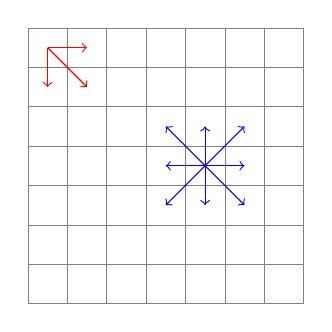
\begin{tikzpicture}[scale=.5]
  \draw[step=1cm,gray,very thin] (-3,-3) grid (4,4);
	\draw[->, red ] (-2.5,3.5) -- (-1.5, 3.5);
	\draw[->, red ] (-2.5,3.5) -- (-1.5, 2.5);
	\draw[->, red ] (-2.5,3.5) -- (-2.5, 2.5);
	\draw[->, blue] (1.5, 0.5) -- (0.5, 0.5);
	\draw[->, blue] (1.5, 0.5) -- (2.5, 0.5);
	\draw[->, blue] (1.5, 0.5) -- (1.5, 1.5);
	\draw[->, blue] (1.5, 0.5) -- (1.5,-0.5);
	\draw[->, blue] (1.5, 0.5) -- (0.5, 1.5);
	\draw[->, blue] (1.5, 0.5) -- (0.5,-0.5);
	\draw[->, blue] (1.5, 0.5) -- (2.5, 1.5);
	\draw[->, blue] (1.5, 0.5) -- (2.5,-0.5);
\end{tikzpicture}
\]
Then a generalized Moore machine of the form $S\yon^S\to p$, where
\[
p= \sum_{(i,j)\in\ord{n}\times\ord{n}}\yon^{d(i)\times d(j)},
\]
is one that has more movement options when it is in the center of the grid than when it is on the sides or corners.
\end{example}

\begin{exercise}
Add to \cref{ex.movement_options} as follows.
\begin{enumerate}
	\item Redefine $p$ so that at each grid value, the robot can receive not only the set of directions it can move in but also a ``reward value'' $r\in\rr$. 
	\item Define the set $S$ of robot states so that an element $s\in S$ includes both the robot's position and a list of all reward values so far.
	\item Define a morphism of polynomials $S\yon^S\to p$ in a way that respects positions and properly updates the robots list of rewards, but otherwise does anything you want.
\qedhere
\end{enumerate}
\end{exercise}

\begin{example}\label{ex.generalized_file_reader}
In \cref{exc.file_reader} one is tasked with making a file reader $\Sys{FileReader}$, where a file is a function $f\colon\ord{n}\to\Set{ascii}$. Now we take that same idea but make the robot have a different interface when it is in read-mode: namely, one where it cannot take in signals.

Let $\State{FileReader} \coloneqq \{(s,t)\mid 1\leq s\leq t\leq n\}$ consist of a
current position $s$ and a terminal position $t$. For our interface, we'll have
two modes, each of which exposes an ascii character:
\[\Out{FileReader} = \present{ \fun{Accepting}(c),\, \fun{Busy}(c) \mid c \in \Set{ascii} }
\]
%%
%% Jaz: In Haskell, this would read
%%      data \Out{FileReader} = Accepting ascii | Busy ascii
%%
For our input, we need a family $\In{FileReader} : \Out{FileReader} \to \smset$.
We'll define this by cases:
\begin{align*}
  \In{FileReader}(\fun{Accepting}(c)) &= \State{FileReader}, \\
  \In{FileReader}(\fun{Busy}(c)) &= \ord{1}.
\end{align*}

Our file reader will be $\fun{Accepting}$ if its current position is the
terminal position; otherwise, it will be $\fun{Busy}$. In either case, it will
expose the ascii character at the current position.
\begin{align*}
  \expose{FileReader}(s, t) = \begin{cases} \fun{Accepting}(f(s)) &\mbox{if $s = t$}\\ \fun{Busy}((f(s)))  \end{cases}
\end{align*}

While the file reader is $\fun{Busy}$, it will step forward through the file.
When it is $\fun{Accepting}$, it will set its new current and terminal position
to be the input. 
\begin{align*}
  \update{FileReader}(s, t) = \begin{cases} \_ \mapsto (s + 1, t) &\mbox{if $\expose{FileReader}(s, t)$ is $\fun{Busy}$} \\ (s', t') \mapsto (s', t') &\mbox{if $\expose{FileReader}(s, t)$ is $\fun{Accepting}$}  \end{cases}
\end{align*}

Let $A\coloneqq\{(s,t)\mid 1\leq s\leq t\leq n\}$, and let $p\coloneqq \Set{ascii}\mdot\yon^A+\Set{ascii}\mdot\yon^\1$; we construct a morphism in $\poly$
\[
(r_1,r^\sharp)\colon A\yon^A\to \Set{ascii}\mdot\yon^A+\Set{ascii}\mdot\yon^\1
\]
as follows.

\[A + B = \langle \fun{inl}(a), \fun{inr}(b) \mid a \in A, b \in B \rangle\]

\[A +_C B = \langle \fun{inl}(a), \fun{inr}(b) \mid a \in A, b \in B, \forall c
\in C.
\fun{inl}(f(c)) = \fun{inr}(g(c)) \rangle\]


On positions define
\[
	r_1(s,t)\coloneqq
	\begin{cases}
		\const{inl}\ f(s)&\tn{ if } s=t\\
		\const{inr}\ f(s)&\tn{ if } s<t
	\end{cases}
\]

\[
	r^\sharp_{(t,t)}(s',t')\coloneqq (s',t')
	\qquad
	r^\sharp_{(s,t)}(1)\coloneqq (s+1,t)
\]
\end{example}

\begin{exercise}
Make a file reader that acts like that in \cref{ex.generalized_file_reader}, except that it only emits output $o\in\Set{ascii}$ when $o=100$.
\end{exercise}

%---- Subsection ----%
\subsection{Wiring diagrams}

We want our dynamical systems to interact with each other.
\begin{equation}\label{eqn.control_diag}
\begin{tikzpicture}[oriented WD, baseline=(B)]
	\node[bb={2}{1}, fill=blue!10] (plant) {\texttt{Plant}};
	\node[bb={1}{1}, below left=-1 and 1 of plant, fill=blue!10]  (cont) {\texttt{Controller}};
	\node[circle, inner sep=1.5pt, fill=black, right=.1] at (plant_out1) (pdot) {};
	\node[bb={0}{0}, inner ysep=25pt, inner xsep=1cm, fit=(plant) (pdot) (cont)] (outer) {};
	\coordinate (outer_out1) at (outer.east|-plant_out1);
	\coordinate (outer_in1) at (outer.west|-plant_in1);
	\begin{scope}[above, font=\footnotesize]
  	\draw (outer_in1) -- node {$A$} (plant_in1);
  	\draw (cont_out1) to node (B) {$B$} (plant_in2);
  	\draw (plant_out1) to node {$C$} (outer_out1);
  	\draw
  		let 
  			\p1 = (cont.south west-| pdot),
  			\p2 = (cont.south west),
  			\n1 = \bby,
  			\n2 = \bbportlen
  		in
  			(pdot) to[out=0, in=0]
  			(\x1+\n2, \y1-\n1) --
  			(\x2-\n2, \y2-\n1) to[out=180, in=180]
  			(cont_in1);
		\end{scope}
	\node[below=0of outer.north] {\texttt{System}};
\end{tikzpicture}
\end{equation}
In this picture the plant is receiving information from the world outside the system, as well as from the controller. It's also producing information for the outside world which is being monitored by the controller.

There are three boxes shown in \eqref{eqn.control_diag}: the controller, the plant, and the system. Each has inputs and outputs, and so we can consider the interface as a monomial.
\begin{equation}\label{eqn.basic_diagram}
	\const{Plant}=C\yon^{AB}
	\qquad\quad
	\const{Controller} = B\yon^C
	\qquad\quad
	\const{System} = C\yon^A.
\end{equation}

The wiring diagram itself is a morphism in $\poly$ of the form
\[
	w\colon\const{Plant}\otimes\const{Controller}\to\const{System}
\]
Since everything involved is a monomial---the parallel product of monomials is a monomial---the whole wiring diagram $w$ is a lens $CB\yon^{ABC}\to C\yon^A$. This morphism says how wires are feeding from outputs to inputs. Like all lenses, it consists of two functions
\[
  \text{get}\colon CB\to C
  \qqand
  \text{put}\colon CBA\to ABC
\]
The first says ``inside the system you have boxes outputting values of type $C$ and $B$. The system needs to produce an output of type $B$; how shall I obtain it?'' The second says ``the system is providing an input value of type $A$, and inside the system you have boxes outputting values of type $C$ and $B$. These boxes need input values of type $A$, $B$, and $C$; how shall I obtain them?'' The answer of course is that \emph{get} is given by projection $(c,b)\mapsto c$ and \emph{put} is given by a permutation $(c,b,a)\mapsto (a,b,c)$. The wiring diagram is a picture that tells us which maps to use.

\begin{exercise}
\begin{enumerate}
	\item Make a new wiring diagram like \eqref{eqn.control_diag} except where the controller also receives information of type $A'$ from the outside world.
	\item What are the monomials in your diagram (replacing \eqref{eqn.basic_diagram})?
	\item What is the morphism of polynomials corresponding to this diagram?
\qedhere
\end{enumerate}
\end{exercise}

Now suppose given a dynamical system in each inner box:
\[
S\yon^S\To{f}\const{Plant}
\qqand
T\yon^T\To{g}\const{Controller}
\]
Then since $\otimes$ is a monoidal product on $\poly$ (see \cref{prop.dirichlet_monoidal}), we get a map
\[
S\yon^S\otimes T\yon^T\To{f\otimes g}\const{Plant}\otimes\const{Controller}
\]
In other words we have a morphism of polynomials $ST\yon^{ST}\to \const{Plant}\otimes\const{Controller}$; that's a new dynamical system with state space $ST=(S\times T)$; a state in it is just a pair of states, one in $S$ and one in $T$. Furthermore our wiring diagram already gave us a map $\const{Plant}\otimes\const{Controller}\to\const{System}$, so combining, we have a new system
\[
ST\yon^{ST}\to\const{System}.
\]

\begin{exercise}
Consider the following wiring diagram.
\[
\begin{tikzpicture}[oriented WD, font=\footnotesize, bb port sep=1, bb port length=2.5pt, bb min width=.4cm, bby=.2cm, inner xsep=.2cm, x=.5cm, y=.3cm, text height=1.5ex, text depth=.5ex]
   	\node[bb={2}{1}, fill=blue!10] (Trf) {$\const{Alice}$};
  	\node[bb={1}{2}, fill=blue!10, below=1 of Trf] (Trg) {$\const{Bob}$};
		\node[bb={2}{2}, fill=blue!10] at ($(Trf)!.5!(Trg)+(1.5,0)$) (Trh) {$\const{Carl}$}; 
  	\node[bb={0}{0}, fit={($(Trf.north west)+(-.25,4)$) (Trg) ($(Trh.north east)+(.25,0)$)}] (Tr) {};
		\node[below] at (Tr.north) {$\const{Team}$};
  	\node[coordinate] at (Tr.west|-Trf_in2) (Tr_in1) {};
  	\node[coordinate] at (Tr.west|-Trg_in1) (Tr_in2) {};
  	\node[coordinate] at (Tr.east|-Trh_out2) (Tr_out1) {};
  	\node at ($(Trg_out2)+(5pt,0)$) (dot) {$\bullet$};
\begin{scope}[font=\tiny]
  	\draw[shorten <=-2pt] (Tr_in1) -- node[below=-3pt] {$A$} (Trf_in2);
  	\draw[shorten <=-2pt] (Tr_in2) -- node[below=-3pt] {$B$} (Trg_in1);
		\draw (Trf_out1) to node[above=-3pt] {$D$} (Trh_in1);
		\draw (Trg_out1) to node[above=-3pt] {$E$} (Trh_in2);
  	\draw (Trg_out2) -- node[below=-3pt] {$F$} (dot.center);
  	\draw[shorten >=-2pt] (Trh_out2) -- node[below=-3pt] {$G$} (Tr_out1);
  	\draw let \p1=(Trh.east), \p2=(Trf.north west), \n1=\bbportlen, \n2=\bby in
  		(Trh_out1) to[in=0] (\x1+\n1,\y2+\n2) -- node[pos=.3, below=-3pt] {$H$} (\x2-\n1,\y2+\n2) to[out=180] (Trf_in1);
	\end{scope}
\end{tikzpicture}
\]
\begin{enumerate}
	\item Write out the polynomials for each of Alice, Bob, and Carl.
	\item Write out the polynomial for the outer box, Team.
	\item The wiring diagram constitutes a morphism $f$ in $\poly$; what is its type $f\colon ?\to ?$
	\item What morphism is it?
	\item Suppose we are given dynamical systems $A\yon^A\to\const{Alice}$, $B\yon^B\to\const{Bob}$, and $C\yon^C\to\const{Carl}$. What is the induced dynamical system on $\const{Team}$?
\qedhere
\end{enumerate}
\end{exercise}

\begin{exercise}[Long division]
\begin{enumerate}
	\item Come up with a function ``divmod'' of type $\nn\times\nn_{\geq1}\to\nn\times\nn$ and which, for example, sends $(10,7)$ to $(1,3)$ and $(30,7)$ to $(4,2)$.
	\item Use \cref{exc.funs_to_moore} to turn it into a dynamical system.
	\item Interpret the following wiring diagram:
\[
\begin{tikzpicture}[oriented WD, bb small]
	\node[bb port sep=3, fill=blue!10, bb={2}{2}] (divmod) {divmod};
	\node[bb={0}{1}, fill=blue!10, left=of divmod_in2] (7) {$7$};
	\node[bb port sep=2, bb={2}{1}, fill=blue!10, below right=-1 and 3 of divmod_out2] (times) {$*$};
	\node[bb={0}{1}, fill=blue!10, below left=-1 and 1 of times_in2] (10) {$10$};
	\node[bb={0}{0}, inner xsep=\bbx, fit=(divmod) (times)(7) (10)] (outer) {};
	\coordinate (outer_in1) at (outer.west|-divmod_in1);
	\coordinate (outer_out1) at (outer.east|-divmod_out1);
	\coordinate (outer_out2) at (outer.east|-times_out1);
	\draw (outer_in1) -- (divmod_in1);
	\draw (7_out1) -- (divmod_in2);
	\draw (10_out1) -- (times_in2);
	\draw (divmod_out1) -- (outer_out1);
	\draw (divmod_out2) to (times_in1);
	\draw (times_out1) -- (outer_out2);
\end{tikzpicture}
\]
	\item Use the above and a diagram of the following form to create a function that spits out the base-10 digits of $1/7$.
\[
\begin{tikzpicture}[oriented WD]
	\node[bb={1}{2}, fill=blue!10] (inner) {};
	\node[bb={0}{0}, inner xsep=1cm, inner ysep=1cm] (outer) {};
	\coordinate (outer_out1) at (outer.east|-inner_out1);
	\draw[shorten >=-3pt] (inner_out1) -- (outer_out1);
	\draw 
		let \p1=(inner.south east), \p2=(inner.south west), \n1=\bbportlen, \n2=\bby in
		(inner_out2) to[in=0] (\x1+\n1,\y1-\n2) -- (\x2-\n1,\y1-\n2) to[out=180] (inner_in1);
		\node[right, font=\footnotesize] at (outer_out1) {$0.142857142857142857\cdots$};
\end{tikzpicture}
\]
\end{enumerate}
\end{exercise}

\begin{exercise}[Cellular automata]\label{exc.cellular_automata}
Let $G=(V,E)$ be a simple graph, i.e.\ $V,E\in\smset$ and $E\ss V\times V$. You can imagine it as a grid 
\[
\begin{tikzcd}[shift left=2pt]
	\LMO{(1,1)}\ar[r]      \ar[d]&
	\LMO{(1,2)}\ar[r]\ar[l]\ar[d]&
	\LMO{(1,3)}\ar[r]\ar[l]\ar[d]&
	\LMO{(1,4)}\ar[r]\ar[l]\ar[d]&
	\LMO{(1,5)}      \ar[l]\ar[d]\\
	\LMO{(2,1)}\ar[r]      \ar[d]\ar[u]&
	\LMO{(2,2)}\ar[r]\ar[l]\ar[d]\ar[u]&
	\LMO{(2,3)}\ar[r]\ar[l]\ar[d]\ar[u]&
	\LMO{(2,4)}\ar[r]\ar[l]\ar[d]\ar[u]&
	\LMO{(2,5)}      \ar[l]\ar[d]\ar[u]\\
	\LMO{(3,1)}\ar[r]      \ar[d]\ar[u]&
	\LMO{(3,2)}\ar[r]\ar[l]\ar[d]\ar[u]&
	\LMO{(3,3)}\ar[r]\ar[l]\ar[d]\ar[u]&
	\LMO{(3,4)}\ar[r]\ar[l]\ar[d]\ar[u]&
	\LMO{(3,5)}      \ar[l]\ar[d]\ar[u]\\
	\LMO{(4,1)}\ar[r]      \ar[d]\ar[u]&
	\LMO{(4,2)}\ar[r]\ar[l]\ar[d]\ar[u]&
	\LMO{(4,3)}\ar[r]\ar[l]\ar[d]\ar[u]&
	\LMO{(4,4)}\ar[r]\ar[l]\ar[d]\ar[u]&
	\LMO{(4,5)}      \ar[l]\ar[d]\ar[u]\\
	\LMO{(5,1)}\ar[r]            \ar[u]&
	\LMO{(5,2)}\ar[r]\ar[l]      \ar[u]&
	\LMO{(5,3)}\ar[r]\ar[l]      \ar[u]&
	\LMO{(5,4)}\ar[r]\ar[l]      \ar[u]&
	\LMO{(5,5)}      \ar[l]      \ar[u]
\end{tikzcd}
\]
finite or infinite, or just an arbitrary graph. For every vertex $v$, the set of vertices $v'$ for which $(v',v)\in E$, i.e.\ for which there is an edge $v'\to v$, is denoted
\[I(v)\coloneq\{v'\mid (v',v)\in E\}.\]
For each $v\in V$, let $p_v\coloneqq \2\yon^{\2^{I(v)}}$; it ``outputs'' a color $\2\cong\{\const{black},\const{white}\}$ and inputs a function $I(v)\to\2$, specifying what all the neighbors are outputting.
\begin{enumerate}
	\item In the drawn grid, what is $I(1,1)$? What is $I(2,2)$?
	\item Specify a morphism $g\colon \bigotimes_{v\in V}p_v\to\yon$ that passes to each vertex $v$ the colors of its neighbors in $I(v)$.
	\item Suppose that for each vertex $v\in V$ you are given a function $f_v\colon 2^{I(v)}\to\2$. Use it to construct a dynamical system $f'_v\colon\2\yon^\2\to p_v$ that updates its state in keeping with $f_v$ and outputs its state directly.
	\item Briefly look up cellular automata in a reference of your choice. Would you say that the dynamical system $\bigotimes_{v\in V}\2\yon^\2\To{\bigotimes f'_v}\bigotimes_{v\in V}p_v\To{g}\yon$ we obtain by wiring together the dynamical systems in the specified way does the same thing as the cellular automata in your reference?
\qedhere
\end{enumerate}
\end{exercise}

%---- Subsection ----%
\subsection{General interaction}

In general, we want systems that can change their interface---remove a port, add a port, change the type of a port, etc.---based on their internal states. But when such systems interact with others, the interaction pattern must be able to accommodate all of the various combinations of interfaces.

\begin{example}
Suppose given two interfaces $p$ and $p'$, having mode sets $M$ and $M'$ respectively
\[
	p\coloneqq \sum_{m\in M} B_m\yon^{A_m}
	\qqand
	p'\coloneqq \sum_{m'\in M'} B'_m\yon^{A'_m}
\]
The parallel product of these is:
\[
p\otimes p'\cong \sum_{(m,m')\in MM'}B_mB'_m\yon^{A_mA'_m}
\]
so the interface $B_mB'_{m'}\yon^{A_mA'_{m'}}$ at each of these $(M\times M')$-many modes $(m,m')$ must be accommodated in any morphism $w\colon p\otimes p'\to q$. For example if $M=\2$ and $M'=\3$ then $w$ can be specified by six maps.
\end{example}

But in fact the possibilities for interaction are much more general than we have led the reader to believe. They may not be broken down into modes at all.

\begin{example}
Let $p\coloneqq B\yon^A$ and $p'=B'\yon^{A'}$. To give a morphism $f\colon p\otimes p'\to \yon$, one specifies a map $B\times B'\to \1$, which is no data, as well as a map $BB'\to AA'$. In other words, for every pair of outputs $(b,b')$ one specifies a pair of inputs $(a,a')$. 

Let's think of elements of $B$ and $B'$ not as outputs, but as positions. 
\[
\begin{tikzpicture}[oriented WD, bb port length=0]
	\node[bb={1}{0}, fill=blue!10, dotted] (p) {$p$};
	\node[bb={1}{0}, fill=blue!10, dotted, below right=-0.5 and 0.5 of p] (q) {$q$};
	\node[bb={0}{0}, inner sep=10pt, fit=(p) (q)] {};
	\node at (p_in1) {\faEye};
	\node at (q_in1) {\faEye};
\end{tikzpicture}
\hspace{.5in}
\begin{tikzpicture}[oriented WD, bb port length=0]
	\node[bb={1}{0}, fill=blue!10, dotted] (p) {$p$};
	\node[bb={1}{0}, fill=blue!10, dotted, below left=-0.5 and 0.5 of p] (q) {$q$};
	\node[bb={0}{0}, inner sep=10pt, fit=(p) (q)] {};
	\node at (p_in1) {\faEye};
	\node at (q_in1) {\faEye};
\end{tikzpicture}
\]
Then given both positions $(b,b')$, the interaction pattern $f$ tells us what the two eyes see, i.e. what values of $(a,a')$ we get.
\end{example}

\begin{example}
Suppose you have two systems $p,q$ each of type $p,q\coloneqq\rr^2\yon^{\rr^2-(0,0)}$. 
\[
\begin{tikzpicture}
	\node (m1) {\faMotorcycle};
	\node[above=-.15 of m1] (e1) {\faEye};
	\node[draw, thick, blue!10, fit = (m1) (e1)] {};
	\node[below right=0 and 1 of m1] (m2) {\scalebox{-1}[1]{\faMotorcycle}};
	\node[above=-.15 of m2] (e2) {\faEye};
	\node[draw, thick, blue!10, fit = (m2) (e2)] {};
\end{tikzpicture}
\]
Taking all pairs of reals except $(0,0)$ corresponds to the fact that the eye cannot see that which is at the same position as the eye.

Let's have the two systems constantly approaching each other with a force equal to the reciprocal of the squared distance between them. If they finally collide, let's have the whole thing come to a halt.

To do this, we want the outer system to be of type $\{\const{go}\}\yon+\{\const{stop}\}$. The morphism $\rr^2\yon^{\rr^2-(0,0)}\otimes\rr^2\yon^{\rr^2-(0,0)}\to\{\const{go}\}\yon+\{\const{stop}\}$ is given on positions by
\[
  \big((x_1,y_1),(x_2,y_2)\big)\mapsto
	\begin{cases}
		(\const{stop},1)&\mbox{ if $x_1=x_2$ and $y_1=y_2$}\\
		(\const{go},1)&\mbox{ otherwise}.
	\end{cases}
\]
On directions, we use the function
\[
  \big((x_1,y_1),(x_2,y_2)\big)\mapsto \big((x_2-x_1,y_2-y_1),(x_1-x_2,y_1-y_2)\big).
\]
Now each system is able to see the vector pointing from it to the other system (unless that vector is zero, in which case the whole thing has halted). Let's use these vectors to define the internal dynamics of each system. Each system will hold as its internal state its current position and velocity, i.e.\ $S=\rr^2\times\rr^2$. To define a map of polynomials $S\yon^S\to\rr^2\yon^{\rr^2-(0,0)}$ we simply output the current position and update the current velocity by adding a vector pointing to the other system and having appropriate magnitude:
\begin{align*}
	\rr^2\times\rr^2&\To{\text{get}}\rr^2\\
	\big((x,y),(x',y')\big)&\Mapsto{\text{get}}(x,y)
\end{align*}
\begin{align*}
	\rr^2\times\rr^2\times(\rr^2-(0,0))&\To{\text{put}}\rr^2\times\rr^2\\
	\big((x,y),(x',y'),(a,b)\big)&\Mapsto{\text{put}}\left(x+x',y+y',x'+\frac{a}{(a^2+b^2)^{3/2}},y'+\frac{b}{(a^2+b^2)^{3/2}}\right)
\end{align*}
\end{example}

\begin{exercise}
Let $p,q\coloneqq\nn\yon^\nn$.
\begin{enumerate}
	\item Write a polynomial morphism $p\otimes q\to\yon$ that corresponds to the function $(a,b)\mapsto (b,a+b)$.
	\item Write dynamical systems $\nn\yon^\nn\to p$ and $\nn\yon^\nn\to q$, each of which simply outputs the previous input.
	\item Suppose each system starts in state $1\in\nn$. What is the trajectory of the $p$-system?
\qedhere
\end{enumerate}
\end{exercise}

\begin{exercise}
Suppose $(X,d)$ is a metric space, i.e.\ $X$ is a set and $d\colon X\times X\to\rr$ is a function satisfying the usual laws. Let's have robots interact in this space.

Let $A,A'$ be sets, each thought of as a set of signals, and let $a_0\in A$ and $a_0'\in A'$ be elements, each thought of as a default value. Let $p\coloneqq AX\yon^{A'X}$ and $p'\coloneqq A'X\yon^{AX}$, and imagine there are two robots, one with interface $p$ and one with interface $p'$.
\begin{enumerate}
	\item Write down a morphism $p\otimes p'\to\yon$ such that each robot receives the other's location, but that it only receives the other's signal when the locations $x,x'$ are sufficiently close, $d(x,x')<1$. Otherwise it receives the default signal.
	\item Write down a morphism $p\otimes p'\to\yon^{[0,5]}$ where the value $s\in [0,5]$ is a scalar, allowing the signal to travel $s$ times further.
	\item Suppose that each robot has a set $S,S'$ of private states. What functions are involved in providing a dynamical system $f\colon SX\yon^{SX}\to AX\yon^{A'X}$?
	\item Change the setup in any way so that the robots only extend a port to hear the other's signal when the distance between them is less than 1. Otherwise, they can only detect the position (element of $X$) that the other currently inhabits.
\qedhere
\end{enumerate}
\end{exercise}

\begin{example}[Cellular automata who vote on their interaction pattern]\label{ex.cell_auto_vote_interaction}
Recall from \cref{exc.cellular_automata} how we constructed cellular automata on a graph $G=(V,E)$. Here $E\ss V\times V$, or equivalently what we might call an \emph{interaction pattern} $I\colon V\to \2^V$, specifies the incoming neighbors $I(v)$ of each $v\in V$.

Suppose now that we are given a function $i\colon V\to\nn$ that we think of as specifying the number $i(v)$ of neighbors each $v\in V$ accepts. Let $\ord{i}(v)=\{1,2,\ldots, i(v)\}$. We will be interested in the polynomial $p_v\coloneqq\2\yon^{\2^{\ord{i}(v)}}$ for each $v$; it represents an interface that outputs a color $\2\cong\{\const{black},\const{white}\}$ and that inputs a function $\ord{i}(v)\to\2$, meant to give the colors of the neighboring vertices.

Say that an interaction pattern $I\colon V\to\2^V$ \emph{respects} $i$ if we have an isomorphism $I(v)\cong\ord{i}(v)$ for each $v\in V$. Suppose given a function $I\colon \2^V\to (\2^V)^V$ such that for each element $s\in\2^V$, the interaction pattern $I_s\colon V\to \2^V$ respects $i$. In the case of \cref{exc.cellular_automata}, $I$ was a constant function. Now we can think of it like all the vertices are voting, via $I$, on the connection pattern. 

We can put this all together by giving a morphism in $\poly$ of the form
\begin{equation}\label{eqn.polymap_misc9237}
\bigotimes_{v\in V}p_v\cong\2^V\yon^{\2^{\sum_{v\in V}\ord{i}(v)}}\too\yon.
\end{equation}
We can such a morphism with a function $g\colon \2^V\to\2^{\sum_{v\in V}\ord{i}(v)}$. Suppose given $s\in\2^V$, so that we have an isomorphism $I_s(v)\cong\ord{i}(v)$ for each $v\in V$; we want a function $g(s)\colon\sum_{v\in V}I_s(v)\to\2$. That is, for each $v$ we want a function
\[
g(s)_v\colon I_s(v)\to\2.
\]
But $I_s(v)\ss V$, so our function $s\colon V\to\2$ induces the desired function $I_s(v)\to\2$.

We have accomplished our goal: the automata vote on their connection pattern. Of course, we don't mean to imply that this vote needs to be democratic or fair in any way: it is an arbitrary function $I\colon \2^V\to(\2^V)^V$. It could be dictated by a given vertex $v_0\in V$ in the sense that its on/off state completely determines the connection pattern $V\times V\to \2$; this would be expressed by saying that $I$ factors as $\2^V\to\2^{v_0}\cong\2\To{I_0}(\2^V)^V$ for some $I_0$.
\end{example}

\begin{exercise}
Change \cref{ex.cell_auto_vote_interaction} slightly by changing the outer box.
\begin{enumerate}
	\item First change it to $A\yon$ for some set $A$ of your choice, and update \eqref{eqn.polymap_misc9237} so that the system outputs some aspect of the current state $\2^V$.
	\item What would it mean to change \eqref{eqn.polymap_misc9237} to a map $\bigotimes_{v\in V}p_v\to\yon^A$ for some $A$?
\qedhere
\end{enumerate}
\end{exercise}

\begin{example}\label{ex.bonds_break}
Recall the picture from \cref{ex.intro_examples_bonds_supplier_assemble}. We said that when too much force is applied to a material, bonds can break. Let's simplify the picture a bit.
\[
\begin{tikzpicture}[oriented WD, bb small, bb port length=0]
	\node[bb={1}{1}, fill=blue!10] (x1) {$\Phi_1$};
	\node[bb={1}{1}, fill=blue!10, right=of x1] (x2) {$\Phi_2$};
	\node[bb={1}{1}, fit= (x1) (x2)] (outer) {};
	\draw[->, shorten >= -4mm] (x1_in1) -- (outer_in1) node[left=4.5mm, font=\tiny] {Force};
	\draw (x1_out1) -- (x2_in1);
	\draw[->, shorten >= -4mm] (x2_out1) -- (outer_out1) node[right=4.5mm, font=\tiny] (L) {Force};
%
	\node[bb={1}{1}, fill=blue!10, right=2in of L] (y1) {$\Phi_1$};
	\node[bb={1}{1}, fill=blue!10, right=of y1] (y2) {$\Phi_2$};
	\node[bb={1}{1}, fit= (y1) (y2)] (outer) {};
	\draw[->, shorten >= -4mm] (y1_in1) -- (outer_in1) node[left=4.5mm, font=\tiny] (R){Force};
	\draw[->, shorten >= -4mm] (y2_out1) -- (outer_out1) node[right=4.5mm, font=\tiny] {Force};
	\node[starburst, draw, minimum width=2cm, minimum height=1.5cm,red,fill=orange,line width=1.5pt] at ($(L)!.5!(R)$)
{Snap!};
\end{tikzpicture}
\]
We will imagine systems $\Phi_1$ and $\Phi_2$ as initially connected in space, that they experience forces from the outside world, and that---for as long as they are connected---they experience forces from each other. More precisely, each internal arena is defined by
\[
	p_1=p_2\coloneqq F\yon^{FF}+\yon^F.
\]
Elements of $F$ will be called \emph{forces}. We need to be able to add and compare forces, i.e.\ we need $F$ to be an ordered monoid; let's say $F=\nn$ for simplicity. The idea is that the arena has two modes: the monomial $F\yon^{FF}$ consisting of two input forces (one from its left and one from its right) and an output force $f_i$, and the monomial $\yon^F$ consisting of one input force (just from the outside). Similarly, in the first mode the system $\Phi_i$ is outputting a force for the other---whether the other uses it or not---but in the second mode the system produces no force for the other.

The external arena is defined to be
\[
p\coloneqq\yon^{FF};
\]
it takes as input two forces $(f_L, f_R)$ and produces unchanging output.

Though the systems $\Phi_1$ and $\Phi_2$ may be initially connected, if the forces on either one surpass a threshold, that system stops sending and receiving forces from the other. The connection is broken and neither system ever receives forces from the other again. This is what we will implement explicitly below.

To do so, we need to create a contract $p_1\otimes p_2\to p$ of the external arena $p$ around (the arenas of) the internal systems. That is, we need to give a morphism of polynomials
\[
\kappa\colon (F\yon^{FF}+\yon^F)\otimes (F\yon^{FF}+\yon^F)\to\yon^{FF}.
\]
By distributivity and the universal property of coproducts, it suffices to give four maps:
\[\arraycolsep=1.4pt
\begin{array}{lll}
	\kappa_{11}\colon&~ FF\yon^{(FF)(FF)}&\to\yon^{FF}\\
	\kappa_{12}\colon&~ F\yon^{(FF)F}&\to\yon^{FF}\\
	\kappa_{21}\colon&~ F\yon^{F(FF)}&\to\yon^{FF}\\
	\kappa_{22}\colon&~ \yon^{FF}&\to\yon^{FF}
\end{array}
\]
The middle two maps $\kappa_{12}$ and $\kappa_{21}$ won't actually occur in our dynamics, so we take them to be arbitrary. We take the last map $\kappa_{22}$ to be an identity (the forces from outside are passed to the two internal boxes). The first map $\kappa_{11}$ is equivalent to a function $(FF)(FF)\to (FF)(FF)$ which we take to be $((f_1,f_2),(f_L,f_R))\mapsto((f_L, f_2),(f_1,f_R))$.

Now that we have the arenas wired together, it remains to give the dynamics on the internal boxes. The states in the two cases will be identical, namely $S\coloneqq F+1$, meaning that at any point the system will either be in the state of holding a force or not. The dynamics will be identical as well, up to a symmetry swapping left and right; let's work with the first. Its interface is $p_1=F\yon^{FF}+\yon^F$ and its dynamics are given by
\[\Phi_1\colon (F+1)\yon^{F+1}\to F\yon^{FF}+\yon^F\]
which splits up as the coproduct of $F\yon^{F+1}\to F\yon^{FF}$ and $\yon^{F+1}\to\yon^F$. The second map corresponds to when the connection is broken; it is given by projection, meaning it just updates the state to be the received force. The first map  $F\yon^{F+1}\to F\yon^{FF}$ corresponds to the case where the system is holding some force, is receiving two input forces and must update its state and produce one output force. For the passforward $F\to F$, let's use identity meaning it outputs the force it's holding. For the passback $F(FF)\to \{\const{Just}\}F+\{\const{Nothing}\}$, let's use the map $(f,(f_L,f_2))\mapsto t(f_L,f_2)$ defined here:
\[
t(f_L,f_2)\coloneqq
\begin{cases}
	\const{Just}~f_L&\tn{ if }f_1+f_2<100\\
	\const{Nothing}&\tn{ otherwise}
\end{cases}
\]
Thus when the sum of forces is high enough, the internal state is updated to the broken state; otherwise it is sent to the force it receives from outside.
\end{example}


\begin{example}\label{ex.supplier_change}
We want to consider the case of a company $C$ that may change its supplier based on its internal state. The company has no output wires, but has two modes of operation---two positions---corresponding to who it wants to receive widgets $W$ from:
\[
\begin{tikzpicture}[oriented WD, every node/.style={fill=blue!10}]
	\node[bb={0}{1}] (s1) {Supplier 1};
	\node[bb={0}{1}, below=of s1] (s2) {Supplier 2};
	\node[bb={1}{0}, right=0.5 of s1] (c) {Company};
	\draw (s1_out1) to node[above, fill=none, font=\tiny] {$W$} (c_in1);
	\draw (s2_out1) to +(5pt,0) node[fill=none] {$\bullet$};
\begin{scope}[xshift=3.5in]
	\node[bb={0}{1}] (s1') {Supplier 1};
	\node[bb={0}{1}, below=of s1'] (s2') {Supplier 2};
	\node[bb={1}{0}, right=0.5 of s2'] (c') {Company};
	\draw (s2'_out1) to node[above, fill=none, font=\tiny] {$W$} (c'_in1);
	\draw (s1'_out1) to +(5pt,0) node[fill=none] {$\bullet$};
\end{scope}
	\node[starburst, draw, minimum width=2cm, minimum height=2cm,align=center,fill=white, font=\small,line width=1.5pt] at ($(c.east)!.5!(s2'.west)$)
{Change\\supplier!};
\end{tikzpicture}
\]
The company has interface $2\yon^W$, and the each supplier has interface $W\yon$; let's take the total system interface (undrawn) to be the closed system $\yon$. Then this mode-dependent wiring diagram is just a map $2\yon^W\otimes W\yon\otimes W\yon\to\yon$. Its on-positions function $2W^2\to1$ is uniquely determined, and its on-directions function $2W^2\to W$ is the evaluation. In other words, the company's position determines which supplier from which it receives widgets.
\end{example}

\begin{example}\label{ex.assemble_machine}
When someone assembles a machine, their own outputs dictate the connection pattern of the machine's components.
\begin{equation}\label{eqn.someone2}
\begin{tikzpicture}[oriented WD, font=\ttfamily, bb port length=0, every node/.style={fill=blue!10}, baseline=(someone.north)]
	\node[bb port sep=.5, bb={0}{1}] (A) {unit A};
	\node[bb port sep=.5, bb={1}{0}, right=of A] (B) {unit B};
	\coordinate (helper) at ($(A)!.5!(B)$);
	\node[bb={1}{1}, below=2 of helper] (someone) {\tikzsymStrichmaxerl[3]};
	\draw[->, dashed, blue] (someone_in1) to[out=180, in=270] (A.270);
	\draw[->, dashed, blue] (someone_out1) to[out=0, in=270] (B.270);
	\draw[->] (A_out1) -- +(10pt,0);
	\draw (B_in1) -- +(-10pt,0);
%
\begin{scope}[xshift=3.5in]
	\node[bb port sep=.5, bb={0}{1}] (A') {unit A};
	\node[bb port sep=.5, bb={1}{0}, right=.5of A'] (B') {unit B};
	\coordinate (helper') at ($(A')!.5!(B')$);
	\node[bb={1}{1}, below=2 of helper'] (someone') {\tikzsymStrichmaxerl[3]};
	\draw[->, dashed, blue] (someone'_in1) to[out=180, in=270] (A'.270);
	\draw[->, dashed, blue] (someone'_out1) to[out=0, in=270] (B'.270);
	\draw[->] (A'_out1) -- (B'_in1);
\end{scope}
%
	\node[starburst, draw, minimum width=2cm, minimum height=2cm,fill=blue!50,line width=1.5pt, align=center, font=\upshape] at ($(B)!.5!(A')-(0,.6cm)$)
{Attach!};
\end{tikzpicture}
\end{equation}
In order for the above picture to make sense, $A$ has the same output that $B$ has as input, say $X$, and we need a default value $x_0\in X$ for $B$ to input when not connected to $A$.

We could say that the person in \eqref{eqn.someone2} has interface $2\yon$, the units have interfaces $X\yon$ and $\yon^X$ respectively, and the whole system is closed; that is, the diagram represents a morphism $2\yon\otimes X\yon\otimes \yon^X\to\yon$. The morphism $2X\yon^X\to\yon$ is uniquely determined on positions, and on directions it is given by cases $(1,x)\mapsto x_0$ and $(2,x)\mapsto x$.
\end{example}

In the above examples we have discussed a very general sort of interaction. One could wonder if it could be made even more general. There indeed may be ideas one could have in mind that simply cannot be expressed in $\poly$: it is only one category.

What's exciting about $\poly$ is that examples like \cref{ex.cell_auto_vote_interaction,ex.assemble_machine} show that it is quite general, and yet as we will see in \cref{sec.bonus_poly}, this single category has excellent formal properties. You can count on it not to crap out. On the spectrum from invention to discovery, $\poly$ itself is a discovery, and its application to dynamics (and later to data and decision) are invention.

%---- Subsection ----%
\subsection{Closure of $\otimes$}

The parallel monoidal product is closed, meaning that there is an operation, which we denote $[-,-]\colon\poly\op\times\poly\to\poly$ and an isomorphism
\[
  \poly(p\otimes q,r)\cong\poly(p,[q,r])
\]
natural in $p,q,r$. The closure operation is defined on $q,r$ as follows:
\begin{equation}\label{eqn.dir_hom}
	[q,r]\coloneqq\prod_{j\in q(\1)}r\circ(q_i\yon)
\end{equation}

\begin{example}\label{ex.double_dual}
For any $A\in\smset$ we have
\[
  [\yon^A,\yon]\cong A\yon
  \qqand
  [A\yon,\yon]\cong\yon^A.
\]
These both follow directly from \eqref{eqn.dir_hom}.
\end{example}

\begin{exercise}
Calculate $[q,r]$ for $q,r\in\poly$ given as follows.
\begin{enumerate}
	\item $q\coloneqq 0$ and $r$ arbitrary.
	\item $q\coloneqq 1$ and $r$ arbitrary.
	\item $q\coloneqq\yon$ and $r$ arbitrary.
	\item $q\coloneqq A$ and $r\coloneqq B$ for $A,B\in\smset$ (constants).
	\item $q\coloneqq A\yon$ and $r\coloneqq B\yon$ for $A,B\in\smset$ (linears).
	\item $q\coloneqq\2\yon^\3+\yon^\2$ and $r\coloneqq\4\yon^\2+\7$.
\qedhere
\end{enumerate}
\end{exercise}

\begin{exercise}
Show that for any $p\in\poly$, if there is an isomorphism $[[p,\yon],\yon]\cong p$, then $p$ is either linear $A\yon$ or representable $\yon^A$ for some $A$. Hint: first show that $p$ must be a monomial.
\end{exercise}

\begin{proposition}\label{prop.dirichlet_closure}
With $[-,-]$ as defined in \eqref{eqn.dir_hom}, there is a natural isomorphism
\begin{equation}\label{eqn.poly_closure_brackets}
	\poly(p\otimes q,r)\cong\poly(p,[q,r]).
\end{equation}
\end{proposition}
\begin{proof}
We have the following chain of natural isomorphisms:
\begin{align*}
	\poly(p\otimes q,r)&\cong
	\poly\Big(\sum_{i\in p(\1)}\sum_{j\in q(\1)}\yon^{p_iq_j},r\Big)\\&\cong
	\prod_{i\in p(\1)}\prod_{j\in q(\1)}\poly(\yon^{p_iq_j},r)\\&\cong
	\prod_{i\in p(\1)}\prod_{j\in q(\1)}r(p_iq_j)\\&\cong
	\prod_{i\in p(\1)}\prod_{j\in q(\1)}\poly(\yon^{p_i},r\circ(q_j\yon))\\&\cong
	\prod_{i\in p(\1)}\poly\Big(\yon^{p_i},\prod_{j\in q(\1)}r\circ(q_j\yon)\Big)\\&\cong
	\poly(p,[q,r]).&
	\qedhere
\end{align*}
\end{proof}

\begin{exercise}\label{exc.poly_plug_1}
Show that for any $p,q$ we have an isomorphism of sets
\[
\poly(p,q)\cong[p,q](\1).
\]
Hint: you can either use the formula \eqref{eqn.dir_hom}, or just use 
\eqref{eqn.poly_closure_brackets} with the Yoneda lemma and the fact that $\yon\otimes p\cong p$.
\end{exercise}


For any $p,q\in\poly$ there is a canonical \emph{evaluation} map
\[
  \fun{eval}\colon [p,q]\otimes p\too q.
\]

\begin{exercise}
\begin{enumerate}
	\item Obtain the evaluation map $\fun{eval}\colon [p,q]\otimes p\too q$ from \eqref{eqn.poly_closure_brackets}.
	\item Show that for any $p,q,r$ and map $f\colon p\otimes q\to r$, there is a unique morphism $f'\colon p\to[q,r]$ such that the following diagram commutes
	\[
	\begin{tikzcd}
		p\otimes q\ar[r, "f'\otimes q"]\ar[rr, bend right, "f"']&
		{[q,r]}\otimes q\ar[r, "\fun{eval}"]&
		r
	\end{tikzcd}
	\]
\qedhere
\end{enumerate}
\end{exercise}

\begin{exercise}
\begin{enumerate}
	\item For any $S$, obtain the map $S\yon^S\to\yon$ whose on-directions map is identity, using eval and \cref{ex.double_dual}.
	\item Show that maps of the four types $\kappa_{11}$, $\kappa_{12}$, $\kappa_{21}$, $\kappa_{22}$ shown in \cref{ex.bonds_break} can be obtained by tensoring together identity maps and eval maps.
\qedhere
\end{enumerate}
\end{exercise}

\begin{example}[Modeling your environment without knowing what it is]
Let's imagine a robot whose interface is an arbitrary polynomial $p$. Let's imagine it is living together in a closed system
\[
	f\colon (q_1\otimes\cdots\otimes q_n)\otimes p\to \yon
\]
with some other robots whose interfaces are $q_1,\ldots,q_n$; let $q\coloneqq(q_1\otimes\cdots\otimes q_n)$. The interaction pattern induces a morphism $f'\colon q\to [p,\yon]$ such that the original system $f$ factors through the evaluation $[p,\yon]\otimes p\to \yon$.

In other words $[p,\yon]$ holds within it all of the possible ways $p$ can interact with other systems in a closed box.%
\footnote{And if you want the generic way $p$ to interact with other systems in a box $r$, just use $[p,r]$.}
To investigate this just a bit, note that $[p,\yon]\cong\prod_{i\in p(\1)}p_i\yon$. That is, for each position in $p$ it produces a direction there, which is just what $p$ needs as input.

Now suppose we were to populate the interface $p$ with dynamics, a map $S\yon^S\to p$. One could aim to choose a set $S$ along with an interesting map $g\colon S\to\poly(p,\yon)$. Then each state $s$ would include a guess $g(s)$ about what the state of the environment is in. This is not the real environment $q$, but just the environment as it affects $p$, namely $[p,\yon]$. The robot's states model environmental conditions.
\end{example}


%-------- Section --------%
\section{Bonus math about the category $\poly$}\label{sec.bonus_poly}

The category $\poly$ has very useful formal properties, including completion under colimits and limits, various adjunctions with $\smset$, factorization systems, and so on. Most of the following material is not necessary for the development of our main story, but we collect it here for reference. The reader can skip directly to \cref{chapter.5} if so inclined. Better yet might be to just gently leaf through \cref{sec.bonus_poly}, to see how well-behaved and versatile the category $\poly$ really is.

%---- Subsection ----%
\subsection{Special polynomials and adjunctions}

There are a few special classes of polynomials that are worth discussing: 
\begin{enumerate}
	\item constant polynomials $\0,\1,\2,A$; 
	\item linear polynomials $\0,\yon, \2\yon, A\yon$;
	\item pure-powers polynomials, $\1, \yon, \yon^\2, \yon^A$; and 
	\item monomials $\0, A, \yon, \2\yon^\3, A\yon^B$.
\end{enumerate}
The first two classes, constant and linear polynomials, are interesting because they both put a copy of $\smset$ inside $\poly$, as we'll see in \cref{prop.ff_const_set_to_poly,prop.ff_lin_set_to_poly}. The third puts a copy of $\smset\op$ inside $\poly$, and the fourth puts a copy of bimorphic lenses inside $\poly$, as we saw in \cref{subsec_prepare_dyn} (page~\pageref{page.bimorphic_lens}).

\begin{exercise}
Which of the four classes above are closed under
\begin{enumerate}
	\item the cocartesian monoidal structure $(\0,+)$?
	\item the cartesian monoidal structure $(\1,\times)$?
	\item the parallel monoidal structure $(\yon,\otimes)$?
	\item composition of polynomials $p\circ q$?%
	\footnote{Composition, together with the unit $\yon$, is in fact yet another monoidal structure, as we will see in \cref{chapter.5}.}
\qedhere
\end{enumerate}
\end{exercise}

\begin{proposition}\label{prop.ff_const_set_to_poly}
There is a fully faithful functor $\smset\to\poly$ sending $A\mapsto A\yon^\0=A$.
\end{proposition}
\begin{proof}
By \cref{eqn.colax_poly_map}, a map $f\colon A\yon^\0\to B\yon^\0$ consists of a function $f\colon A\to B$ and for each $a\in A$ a function $\0\to\0$. There is only one such function, so $f$ can be identified with just a map of sets $A\to B$.
\end{proof}

\begin{proposition}\label{prop.ff_lin_set_to_poly}
There is a fully faithful functor $\smset\to\poly$ sending $A\mapsto A\yon$.
\end{proposition}
\begin{proof}
By \cref{eqn.colax_poly_map}, a map $f\colon A\yon^\1\to B\yon^\1$ consists of a function $f\colon A\to B$ and for each $a\in A$ a function $\1\to\1$. There is only one such function, so $f$ can be identified with just a map of sets $A\to B$.
\end{proof}

\begin{theorem}\label{thm.adjoint_quadruple}
$\poly$ has an adjoint quadruple with $\smset$:
\begin{equation}\label{eqn.adjoints_galore}
\begin{tikzcd}[column sep=60pt, background color=theoremcolor]
  \smset
  	\ar[r, shift left=7pt, "A" description]
		\ar[r, shift left=-21pt, "A\yon"']&
  \poly
  	\ar[l, shift right=21pt, "p(\0)"']
  	\ar[l, shift right=-7pt, "p(\1)" description]
	\ar[l, phantom, "\scriptstyle\Leftarrow"]
	\ar[l, phantom, shift left=14pt, "\scriptstyle\Rightarrow"]
	\ar[l, phantom, shift right=14pt, "\scriptstyle\Rightarrow"]
\end{tikzcd}
\end{equation}
where the functors have been labeled by where they send $A\in\smset$ and $p\in \poly$. 

Both rightward functors are fully faithful.
\end{theorem}
\begin{proof}
For any set $A$, there is a functor $\poly\to\smset$ given by sending $p$ to $p(A)$; it is $\poly(A,-)$. This, together with \cref{prop.ff_const_set_to_poly,prop.ff_lin_set_to_poly} give us the four functors and the fact that the two rightward functors are fully faithful. It remains to provide the following three natural isomorphisms:
\[
\smset(A,p(\0))\cong\poly(A,p)\qquad
\smset(p(\1),A)\cong\poly(p,A)\qquad
\smset(A,p(\1))\cong\poly(A\yon,p).
\]
All three come from our main formula, \cref{eqn.main_formula}; we leave the details to the reader in \cref{exc.adjoint_quadruple}.
\end{proof}

\begin{exercise}\label{exc.adjoint_quadruple}
Here we prove the remainder of \cref{thm.adjoint_quadruple} using \cref{eqn.main_formula}:
\begin{enumerate}
	\item Provide a natural isomorphism $\smset(A,p(\0))\cong\poly(A,p)$.
	\item Provide a natural isomorphism $\smset(p(\1),A)\cong\poly(p,A)$.
	\item Provide a natural isomorphism $\smset(A,p(\1))\cong\poly(A\yon,p)$.
\qedhere
\end{enumerate}
\end{exercise}

In \cref{thm.adjoint_quadruple} we see that $p\mapsto p(\0)$ and $p\mapsto p(\1)$ have left adjoints. This is true more generally for any set $A$ in place of $\0$ and $\1$, as we show in \cref{cor.substituting_adj}. However, the fact that $p\mapsto p(\1)$ is also a right adjoint---and hence that we have the \emph{quadruple} of adjunctions in \eqref{eqn.adjoints_galore}---is special to $A=\0,\1$.

Next we note that the set of polynomial morphisms $p\to q$ 

\begin{proposition}\label{prop.two_var_adj}
There is a two-variable adjunction between $\smset$, $\poly$, and $\poly$:%
\footnote{The first set $\poly(Ap,q)$ involves the $A$-fold coproduct of $p$ and the middle set $\poly(p,q^A)$ involves the $A$-fold product of $q$, neither of which we have proven exists. For organizational purposes, we put that off until \cref{prop.coprod_prod_poly}.
}
\begin{align}\label{eqn.two_var_adj}
\poly(Ap,q)\cong\poly(p,q^A)\cong\smset(A,\poly(p,q)).
\end{align}
\end{proposition}
\begin{proof}
Since $Ap$ is the $A$-fold coproduct of $p$ and $q^A$ is the $A$-fold product of $q$, the universal properties of coproduct and product give isomorphisms
\[\poly(Ap,q)\cong\prod_{a\in A}\poly(p,q)\cong\poly(p,q^A).\]
The middle set is in bijection with $\smset(A,\poly(p,q))$, completing the proof.
\end{proof}

Replacing $q$ with $p$ and replacing $p$ with $\yon^B$ in \cref{prop.two_var_adj}, we obtain the following using the Yoneda lemma.

\begin{corollary}\label{cor.substituting_adj}
For any set $B$ there is an adjunction
\[
\adj{\smset}{A\yon^B}{p(B)}{\poly}
\]
where the functors are labeled by where they send $p\in\poly$ and $A\in\smset$.
\end{corollary}

\begin{exercise}
Prove \cref{cor.substituting_adj} from \cref{prop.two_var_adj}.
\end{exercise}

\begin{proposition}
The Yoneda embedding $A\mapsto \yon^A$ has a left adjoint
\[
\adjr{\smset\op}{\yon^-}{\Gamma}{\poly}
\]
where $\Gamma(p)\coloneqq\prod_{i\in p(\1)}p_i$.
\end{proposition}
\begin{proof}
We have the following chain of natural isomorphisms:
\begin{align*}
  \smset(A,\Gamma(p))&\cong
  \Big(\prod_{i\in p(\1)}p_i\Big)^A
  	&\text{Definition of function}\\&\cong
  \prod_{i\in p(\1)}{p_i}^A
  	&\text{Definition of product}\\&\cong
  \prod_{i\in p(\1)}\sum_{j\in\1}{p_i}^A
  	&\text{Trivial sum}\\&\cong
  \poly(p,\yon^A).&\cref{eqn.main_formula}
\end{align*}

\end{proof}

\begin{exercise}
Show that $\Gamma(p)\cong[p,\yon](\1)$ where $[-,-]$ is as in \cref{prop.dirichlet_closure}.
\end{exercise}

\paragraph{Epi-mono factorization.}

\begin{proposition}
Let $(f_1,f^\sharp)\colon p\to q$ be a morphism in $\poly$. It is a monomorphism iff the function $f_1\colon p(\1)\to q(\1)$ is a monomorphism in $\smset$ and, for each $i\in p(\1)$ the function $f_i^\sharp\colon q_{f_1(i)}\to p_i$ is an epimorphism in $\smset$.
\end{proposition}
\begin{proof}
\noindent$\Rightarrow$: Suppose that $f$ is a monomorphism. Since $p\mapsto p(\1)$ is a right adjoint (\cref{thm.adjoint_quadruple}), it preserves monomorphisms. We need to show that for any $i\in p(\1)$ the function $f_i^\sharp\colon q_{f_1(i)}\to p_i$ is an epimorphism in $\smset$. Suppose given a set $A$ and a pair of functions $g^\sharp,h^\sharp\colon p_i\tto A$ with $g^\sharp f_i^\sharp=h^\sharp f_i^\sharp$. They can be identified with morphisms $\yon^A\tto p$ whose compositions with $f$ are equal, hence $g=h$ by assumption, and hence $g^\sharp=h^\sharp$ as desired.

\noindent$\Leftarrow$: Suppose that $f_1$ is a monomorphism and that for each $i\in p(\1)$ the function $f_i^\sharp$ is an epimorphism. Let $r$ be a polynomial, $g,h\colon r\tto p$ two morphisms, and suppose $fg=fh$. Then $f_1g_1=f_1h_1$, which implies $g_1=h_1$; we'll consider $g_1$ the default representation. We also have that $g^\sharp_kf^\sharp_{g_1k}=h^\sharp_kf^\sharp_{g_1k}$ for any $k\in r(\1)$. But $f^\sharp_{g_1k}$ is an epimorphism, so in fact $g^\sharp_k=h^\sharp_k$, as desired.
\end{proof}

\begin{proposition}
Let $(f_1,f^\sharp)\colon p\to q$ be a morphism in $\poly$. It is an epimorphism iff the function $f_1\colon p(\1)\to q(\1)$ is an epimorphism in $\smset$ and, for each $j\in q(\1)$ the induced function 
\[
f^\flat_j\colon q_j\to\prod_{\{i\in p(\1)\,\mid\, f_1(i)=j\}}p_i
\]
from \eqref{eqn.useful_misc472} is a monomorphism.
\end{proposition}
\begin{proof}
\noindent$\Rightarrow$: Suppose that $f$ is an epimorphism. Since $p\mapsto p(\1)$ is a left adjoint (\cref{thm.adjoint_quadruple}), it preserves epimorphisms. We need to show that for any $j\in q(\1)$ the  function $f^\flat_j$ is a monomorphism in $\smset$. Suppose given a set $A$ and a pair of functions $g^\sharp,h^\sharp\colon A\tto q_j$ with $f^\flat_jg^\sharp=f^\flat_jh^\sharp$. They can be identified with morphisms $g,h\colon q\tto \yon^A+\1$, which send the $j$-component to the first component, $\yon^A$, and send all other component to the second component, $\1$. It is easy to check that $fg=fh$, hence $g=h$, and hence $g^\sharp=h^\sharp$ as desired.

\noindent$\Leftarrow$: Suppose that $f_1$ is an epimorphism and that for each $j\in q(\1)$ the function $f^\flat_j$ is a monomorphism. Let $r$ be a polynomial, $g,h\colon q\tto r$ two morphisms, and suppose $gf=hf$. Then $g_1f_1=h_1f_1$, which implies $g_1=h_1$; we'll consider $g_1$ the default representation. We also have that $f^\sharp_ig^\sharp_{fi}=f^\sharp_ih^\sharp_{fi}$ for any $i\in p(\1)$. Then, in particular, for any $j\in q(\1)$ the two composites
\[
\begin{tikzcd}
	r_{g_1j}\ar[r, shift left, "g^\sharp_j"]\ar[r, shift right, "h^\sharp_j"']&q_j\ar[r, "f^\flat_j"]&\displaystyle\prod_{\{i\in p(\1)\,\mid\,f_1(i)=j\}}p_i
\end{tikzcd}
\]
are equal, which implies that $g^\sharp_j=h^\sharp_j$ as desired.
\end{proof}

\begin{exercise}
Suppose $f$ is both a mono and an epi; it is an iso? (That is, is $\poly$ \emph{balanced}?)
\end{exercise}

\begin{exercise}[Epi-mono factorization]\label{exc.mono_epi_poly}
Suppose $p,q\in\poly$ are polynomials and $f=(f_1,f^\sharp)\colon p\to q$ is a morphism with notation as in \cref{eqn.colax_poly_map}.
\begin{enumerate}
	\item Can every morphism in $\poly$ be factored as an epic followed by a monic?
	\item Is your factorization unique up to isomorphism?
\qedhere
\end{enumerate}
\end{exercise}



%---- Subsection ----%
\subsection{Limits, colimits, and cartesian closure}

We will now see that $\poly$ has all limits and colimits, and moreover it is cartesian closed.

Let's begin with something fairly simple: that $+$ gives a coproduct in $\poly$. We could have said this elementary fact much earlier, but we were in a rush to get to the applications in \cref{sec.dynam_in_poly}.

\begin{exercise}
Show that the category $\poly$ has finite coproducts as follows.
\begin{enumerate}
	\item Show that $\0$ is an initial object in $\poly$, i.e.\ that for any polynomial $p$ there is a unique morphism $\0\to p$.
	\item Show that the standard sum of polynomials $p_1+p_2$ is a coproduct of $p_1$ and $p_2$. That is, provide morphisms $p_1\to p_1+p_2\from p_2$ and show that for any other $q$ with morphisms $p_1\To{f_1} q\From{f_2} p_2$, there exists a unique morphism $p_1+p_2\to q$---shown dashed---making the following diagram commute 
	\[
	\begin{tikzcd}
		p_1\ar[r]\ar[dr, "f_1"']&
		p_1+p_2\ar[d, dashed]&
		p_2\ar[l]\ar[dl, "f_2"]\\&
		q
	\end{tikzcd}
	\qedhere
	\]
\end{enumerate}
\end{exercise}

The general case of coproducts and products is not much more difficult.

\begin{proposition}\label{prop.coprod_prod_poly}
The category $\poly$ has coproducts and products.
\end{proposition}
\begin{proof}
Let $A$ be a set and $p\colon A\to\poly$ a collection of polynomials $(p_a)_{a\in A}$.%
\footnote{
This is potentially ambiguous notation because $p_i$ generally denotes the exponent of the $i$th summand of polynomial $p$; we apologize for this. To be clear, to each $a\in A$ there is an associated polynomial $p_a\in\poly$. To write out $p_a$ as a sum of representables, we would say $p_a=\sum_{i\in p_a(\1)}\yon^{(p_a)_i}$.
}
Their coproduct is
\begin{equation}\label{eqn.sum_polys}
\sum_{a\in A}p_a=\sum_{a\in A}\sum_{i\in p_a(\1)}\yon^{(p_a)_i}\cong\sum_{(a,i)\in\sum_{a\in A}p_a(\1)}\yon^{(p_a)_i}
\end{equation}
which is manifestly a sum of representables, i.e.\ a polynomial, and which one can check satisfies the universal property of coproduct; see \cref{exc.check_coprod_prod}.

We claim that the product of this collection is
\begin{equation}\label{eqn.prod_polys}
\prod_{a\in A}p_a=
\prod_{a\in A}\sum_{i\in p_a(\1)}\yon^{(p_a)_i}\cong
\sum_{i\colon \prod_{a\in A}p_a(\1)}\yon^{\sum_{a\in A}p_{i(a)}}.
\end{equation}
Again, it is a sum of representables, so a polynomial, and one can check that it satisfies the universal property of product; see \cref{exc.check_coprod_prod}.
\end{proof}

\begin{exercise}\label{exc.check_coprod_prod}
Finish the proof of \cref{prop.coprod_prod_poly} as follows.
\begin{enumerate}
	\item Show that \eqref{eqn.sum_polys} satisfies the universal property for coproduct of polynomials.
	\item Show that \eqref{eqn.prod_polys} satisfies the universal property for product of polynomials.
\qedhere
\end{enumerate}
\end{exercise}

\begin{exercise}
Let $A=\2$ and $p\colon A\to\poly$ be given by $p_1\coloneqq\yon+\1$ and $p_2\coloneqq\yon+\2$. What is $\prod_{i\in\2}p_i$ according to \cref{eqn.prod_polys}? Does it check out?
\end{exercise}

\begin{proposition}\label{prop.completely_distributive}
The category $\poly$ is completely distributive, i.e.\ for any set $A$, sets $(B_a)_{a\in A}$, and polynomials $(p_{(a,b)})_{a\in A, b\in B_a}$, there is an isomorphism
\[
  \sum_{b\colon\prod_{a\in A}B(a)}\;\prod_{a\in A}\;p_{(a,b(a))}
  \cong
	\prod_{a\in A}\;\sum_{b\in B(a)}\;p_{(a,b)}
\]
\end{proposition}
\begin{proof}
By the universal property of coproducts and products, to provide a morphism $\sum_{b\colon\prod_{a\in A}B(a)}\prod_{a\in A}p_{(a,b)}
  \to	\prod_{a\in A}\sum_{b\in B(a)}p_{(a,b)}$, it suffices to fix an arbitrary $b_0\in\prod_{a\in A}B(a)$ and $a_0\in A$ and provide a morphism $\prod_{a\in A}p_{(a,b_0(a))}\to\sum_{b\in B(a_0)}p_{(a_0,b)}$. We do so by first projecting onto the $a_0$-factor $\prod_{a\in A}p_{(a,b_0(a))}\to p_{(a_0, b_0(a_0))}$ and then including into the $b_0(a_0)$-summand $p_{(a_0,b_0(a_0))}\to\sum_{b\in B(a_0)}p_{(a_0,b)}$. This establishes the morphism.
  
  To see that it is an isomorphism in $\poly$, i.e.\ a natural isomorphism of functors, it suffices to check it on components. So fix $X\in\smset$. The induced map
  \[
  \sum_{b\colon\prod_{a\in A}B(a)}\;\prod_{a\in A}\;p_{(a,b(a))}
  \cong
	\prod_{a\in A}\;\sum_{b\in B(a)}\;p_{(a,b)}
  \]
  is exactly as in \cref{prop.push_prod_sum_set}, which we proved is an isomorphism. This completes the proof.
\end{proof}

\begin{exercise}
How is the usual distributive law,
\[
p(q+r)\cong pq+pr
\]
for $p,q,r\in\poly$, a special case of \cref{prop.completely_distributive}?
\end{exercise}

\paragraph{Cartesian closure}
For any two polynomials $q,r$, define $r^q\in\poly$ by the following formula
\begin{equation}\label{eqn.exponential}
  r^q\coloneqq\prod_{i\in q(\1)}r\circ(\yon+q_j)
\end{equation}
where $\circ$ denotes composition.

Before proving that this really is an exponential in $\poly$, which we do in \cref{thm.poly_cart_closed}, we first get some practice with it.

\begin{example}
Let $A$ be a set. We've been writing the polynomial $A\yon^\0$ simply as $A$ and the polynomial $\yon^\1$ simply as $\yon$, so it better be true that the there is an isomorphism 
\[\yon^A\cong (\yon^\1)^{(A\yon^\0)}\]
in order for the notation to be consistent. Luckily, this is true. Checking \eqref{eqn.exponential}, we have
\[(\yon^\1)^{A\yon^\0}=\prod_{a\in A}\yon\circ(\0+\yon)\cong\yon^A\]
\end{example}

\begin{exercise}
Compute the following exponentials in $\poly$ using \eqref{eqn.exponential}:
\begin{enumerate}
	\item $p^\0$ for an arbitrary $p\in\poly$.
	\item $p^\1$ for an arbitrary $p\in\poly$.
	\item $\1^p$ for an arbitrary $p\in\poly$.
	\item $A^p$ for an arbitrary $p\in\poly$ and $A\in\smset$.
	\item $\yon^\yon$.
	\item $\yon^{\4\yon}$.
	\item $(\yon^A)^{\yon^B}$ for arbitrary sets $A,B\in\smset$.
\qedhere
\end{enumerate}
\end{exercise}


\begin{theorem}\label{thm.poly_cart_closed}
The category $\poly$ is Cartesian closed. That is, we have a natural isomorphism
\[
  \poly(p,r^q)\cong\poly(p\times q,r),
\]
where $r^q$ is the polynomial defined in \eqref{eqn.exponential}.
\end{theorem}
\begin{proof}
We have the following chain of natural isomorphisms
\begin{align*}
	\poly(p,r^q)&\cong
	\poly\Big(p,\prod_{j\in q(\1)}r\circ (\yon+q_j)\Big)\\&\cong
	\prod_{j\in q(\1)}\poly(p,r\circ(\yon+q_j))\\&\cong
	\prod_{j\in q(\1)}\prod_{i\in p(\1)}\poly(\yon^{p_i},r\circ(\yon+q_j))\\&\cong
	\prod_{i\in p(\1)}\prod_{j\in q(\1)}r\circ(p_i+q_j)\\&\cong
	\prod_{i\in p(\1)}\prod_{j\in q(\1)}\sum_{k\in r(\1)}(p_i+q_j)^{r_k}\\&\cong
	\poly(p\times q,r).
\end{align*}
The last step uses \cref{eqn.main_formula,prop.poly_times}.
\end{proof}


\begin{exercise}
Using \cref{eqn.exponential}, show that the functor $\smset\to\poly$ sends exponentials to exponentials.
\end{exercise}

\begin{theorem}\label{thm.poly_limits}
The category $\poly$ has all limits.
\end{theorem}
\begin{proof}
Recall that a category has all limits iff it has equalizers and products, so by \cref{prop.coprod_prod_poly} it suffices to show that $\poly$ has equalizers. 

Let $f_1,f_2\colon p\tto q$ be two maps of polynomials. Let $E\to p(\1)\tto q(\1)$ be an equalizer of the functions $f_1(\1),$ and $f_2(\1)$ in $\smset$. For each $e\in E$, write $f(e)\coloneqq f_1(e)=f_2(e)$; we have two polynomial morphisms $\yon^{p_e}\tto\yon_{q_{f(e)}}$, i.e.\ two functions $q_{f(e)}\tto p_e$. Defining $p'_e\in\smset$ to be their coequalizer, we can define a polynomial $p'$ as follows:
\[
  p'\coloneqq\sum_{e\in E}\yon^{p'_e}
\]
which comes equipped with a morphism $g\colon p'\to p$. One can check that it is an equalizer of $f_1,f_2$; see \cref{exc.poly_limits}.
\end{proof}

\begin{exercise}\label{exc.poly_limits}
Complete the proof of \cref{thm.poly_limits} as follows:
\begin{enumerate}
	\item We said that $p'$ comes equipped with a morphism $g\colon p'\to p$; what is it?
	\item Show that $g\then f_1=g\then f_2$.
	\item Show that $g$ is an equalizer of the pair $f_1,f_2$.
\qedhere
\end{enumerate}
\end{exercise}

\begin{exercise}
Let $p$ be any polynomial.
\begin{enumerate}
	\item There is a canonical choice of morphism $\eta\colon p\to p(\1)$; what is it?
	\item Suppose given an element $i\in p(\1)$, i.e.\ a function $\1\to p(\1)$.
	\item What is the pullback
	\[
	\begin{tikzcd}
	?\ar[r]\ar[d]&
	p\ar[d, "\eta"]\\
	\1\ar[r, "i"']&
	p(\1)\ar[ul, phantom, very near end, "\lrcorner"]
	\end{tikzcd}
	\qedhere
	\]
\end{enumerate}
\end{exercise}

\begin{example}[Pullbacks in $\poly$]\label{ex.pullbacks_in_poly}
Given polynomials $q,q',r$ and dependent lenses $q\To{f} r\From{f'} q'$, the pullback 
\[
\begin{tikzcd}
	p\ar[r]\ar[d]&
	q'\ar[d, "f'"]\\
	q\ar[r, "f"']&
	r\ar[ul, phantom, very near end, "\lrcorner"]
\end{tikzcd}
\]
 is given as follows. The set of positions in $p$ is the pullback of the positions of $q$ and $q'$ over those of $r$. On each position $(i, i')$ with $f_1(i)=f'_1(i')$, we take the directions set of $p$ in that position to be the  pushout of the directions $q_i$ and $q'_{i'}$ over $r_{f_1(i)}=r_{f_1'(i')}$:
\begin{equation}\label{eqn.pullback_poly}
\begin{tikzcd}
	p(\1)\ar[r]\ar[d]&
	q'(\1)\ar[d, "f_1'"]\\
	q(\1)\ar[r, "f_1"']&
	r(\1)\ar[ul, phantom, very near end, "\lrcorner"]
\end{tikzcd}
\qqand
\begin{tikzcd}
	p_{(i,i')}\ar[r]\ar[d]&
	q'_{i'}\ar[d, "(f')_{i'}^\sharp"]\\
	q_i\ar[r, "f^\sharp_i"']&
	r_{f_1(i)}\ar[from = ul, phantom, very near end, "\ulcorner"]
\end{tikzcd}
\end{equation}
\end{example}

\begin{exercise}
Let $q\coloneqq \yon^\2+\yon$, $q'\coloneqq\2\yon^\3+\yon^\2$, and $r\coloneq\yon+\1$.
\begin{enumerate}
	\item Choose morphisms $f\colon q\to r$ and $f'\colon q'\to r$ and write them down.
	\item Find the pullback of your diagram.
\qedhere
\end{enumerate}
\end{exercise}

Arbitrary colimits will be much less useful to us than limits, so the following theorem is included only for completeness; the reader can feel free to skip it.
\begin{theorem}\label{thm.poly_colimits}
The category $\poly$ has all colimits.
\end{theorem}
\begin{proof}
Recall that a category has all colimits iff it has coequalizers and coproducts, so by \cref{prop.coprod_prod_poly} it suffices to show that $\poly$ has coequalizers.

Let $f_1,f_2\colon p\tto q$ be two maps of polynomials. The pair of functions
\[f_1(\1),f_2(\1)\colon p(\1)\tto q(\1)\] 
define a graph $G\colon\fbox{$\bullet\tto\bullet$}\to\smset$ whose set $C$ of connected components is given by the coequalizer $g\colon q(\1)\to C$ of $f_1(\1)$ and $f_2(\1)$. The coequalizer of $f_1$ and $f_2$ will turn out to be a $C$-indexed sum of representables, each of which is given by a limit of a diagram of representables from $p$ and $q$, but expressing this limit, as we proceed to do, is a bit involved.

For each connected component $c\in C$, we have a connected subgraph $G_c\ss G$ with vertices $V_c\coloneqq g\inv(c)$ and edges $E_c\coloneqq f_1\inv(g\inv(c))=f_2\inv(g\inv(c))$. Note that $E_c\ss p(\1)$ and $V_c\ss q(\1)$, so to each $e\in E_c$ (resp.\ to each $v\in V_c$) we have an associated representable $\yon^{p_e}$ (resp.\ $\yon^{q_v}$).

The category of elements $\int G_c$ is a bipartite graph with objects $V+E$ and with two sorts of morphisms, $e\to f_1(e)$ and $e\to f_2(e)$, associated to each $e\in E_c$; all non-identity arrows point from an object in $E$ to an object in $V$. There is a functor $F\colon(\int G_c)\op\to\smset$ sending every $v\mapsto q_v$, every $e\mapsto p_e$, and every morphism to a function between them, namely either $(f_1^\sharp)_e\colon q_{f_1(e)}\to p_e$ or $(f_2^\sharp)_e\colon q_{f_2(e)}\to p_e$. Define $q'_c\in\smset$ to be the limit $q'_c\coloneqq\lim F\in\smset$ of $F$.

We claim that $q'\coloneqq\sum_{c\in C}\yon^{q'_c}$ is the coequalizer of $f_1$ and $f_2$. We leave the completion proof to the interested reader in \cref{exc.poly_colimits}.
\end{proof}

\begin{exercise}\label{exc.poly_colimits}
Complete the proof of \cref{thm.poly_colimits} as follows:
\begin{enumerate}
	\item Provide a map $g\colon q\to q'$ and show that $f_1\then g=f_2\then g$.
	\item Show that $g$ is a coequalizer of the pair $f_1,f_2$.
\qedhere
\end{enumerate}
\end{exercise}


%---- Subsection ----%
\subsection{Monoidal $*$-bifibration over $\smset$}

We will see that the functor $p\mapsto p(\1)$ has special properties making it what
\cite{shulman2008framed} refers to as a \emph{monoidal $*$-bifibration}. This means that $\smset$ acts as a sort of remote controller on the category $\poly$, grabbing every polynomial by its positions and pushing or pulling it this way and that. 

For example, suppose one has a set $A$ and a function $f\colon A\to p(\1)$. Then we get a new polynomial $f^*p$ with positions $A$. The notation here agrees with that in \cref{thm.poly_lcc}: it is given by a pullback
\[
\begin{tikzcd}
	f^*p\ar[r, "\fun{cart}"]\ar[d]&
	p\ar[d, "\eta_p"]\\
	A\ar[r, "f"']&
	p(\1)\ar[ul, phantom, very near end, "\lrcorner"]
\end{tikzcd}
\]
Here $\eta_p$ is the unit of the adjunction $\adjr{\smset}{A}{p(\1)}{\poly}$. Since it is an isomorphismon positions and $p\mapsto p(\1)$ is a right adjoint, the map $f^*p\to A$ is also an isomorphism on positions. Since on each position $a\in A$, the function $f^\sharp_a$ is an isomorphism on directions (both domain and codomain are the empty set), and since the $a$-position of $f^*p$ is constructed by a pushout (see \cref{ex.pullbacks_in_poly}), each function $\fun{cart}_a^\sharp\colon p_{f(a)}\to(f^*p)_a$ is an isomorphism too.

\begin{definition}[Vertical, cartesian]
Let $f\colon p\to q$ be a morphism of polynomials. It is called \emph{vertical} if $f_1\colon p(\1)\to q(\1)$ is an isomorphism. It is called \emph{cartesian} if, for each $i\in p(\1)$ the function $f^\sharp_i\colon q_{f(i)}\to p_i$ is an isomorphism.
\end{definition}

\begin{proposition}\label{prop.vert_cart_factorization}
Every morphism in $\poly$ can be uniquely factored as a vertical morphism followed by a cartesian morphism.
\end{proposition}
\begin{proof}
Recall from \cref{eqn.colax_poly_map} that a morphism in $\poly$ can be written as to the left; we can thus rewrite it as to the right:
\[
\begin{tikzcd}[column sep=small]
	p(\1)\ar[dr, bend right, "p_-"']\ar[rr, "f_1"]&~&
	q(\1)\ar[dl, bend left, "q_-"]\\&
	\smset\ar[u, phantom, near end, "\overset{f^\sharp}{\Leftarrow}"]
\end{tikzcd}
\hspace{1in}
\begin{tikzcd}
	p(\1)\ar[dr, bend right, "p_-"']\ar[r, equal, ""' name=equal]&
	p(\1)\ar[d, "q_{f_1(-)}" description]\ar[r, "f_1"]&
	q(\1)\ar[dl, bend left, "q_-"]\\&
	|[alias=set]|\smset\ar[from=equal, to=set, pos=.3, phantom, "\overset{f^\sharp}{\Leftarrow}"]
\end{tikzcd}
\]
The object $\lens{q_{f_1i}}{i\in p(\1)}$ is clearly unique up to isomorphism.
\end{proof}

\begin{proposition}\label{prop.monoidal_pres_carts}
The monoidal structures $+$, $\times$, and $\otimes$ preserve cartesian morphisms.
\end{proposition}
\begin{proof}
Suppose that  $f\colon p\to p'$ and $g\colon q\to q'$ are cartesian. 

A position of $p+q$ is a position $i\in p(\1)$ or a position $j\in q(\1)$, and the map $(f+g)^\sharp$ at that position is either $f^\sharp_i$ or $g^\sharp_j$; either way it is an isomorphism, so $f+g$ is cartesian.

A position of $p\times q$ (resp.\ of $p\otimes q$) is a pair $(i,j)\in p(\1)\times q(\1)$. The morphism $(f\times g)^\sharp_{i,j}$ is $f^\sharp_i+g^\sharp_j$ (resp.\ $f^\sharp_i\times g^\sharp_j$) which is again an isomorphism if $f^\sharp_i$ and $g^\sharp_j$ are. Hence $f\times g$ (resp.\ $f\otimes g$) is cartesian, completing the proof.
\end{proof}

\begin{theorem}[Cartesian morphisms in $\poly$ are exponentiable]\label{thm.cart_exponentiable}
If $f\colon p\to q$ is cartesian then the functor $f^*\colon\poly/q\to\poly/p$ given by pulling back $q'\to q$ along $f$ is a left adjoint:
\[
\begin{tikzcd}[column sep=50pt, background color=theoremcolor]
	\poly/p\ar[r, shift right=7pt, "f_*"']&
	\poly/q\ar[l, shift right=7pt, "f^*"']\ar[l, phantom, "\Rightarrow"]
\end{tikzcd}
\]
\end{theorem}
\begin{proof}
Fix $e\colon p'\to p$ and $g\colon q'\to q$.
\[
\begin{tikzcd}
	p'\ar[d, "e"']&q'\ar[d, "g"]\\
	p\ar[r, "f"']&q.
\end{tikzcd}
\]
We need to define a functor $f_*\colon\poly/p\to\poly/q$ and prove the analogous isomorphism establishing it as right adjoint to $f^*$. We first establish some notation. Given a set $Q$ and sets $(P'_i)_{i\in I}$, each equipped with a map $Q\to P'_i$, let $Q/\sum_{i\in I}P'_i$ denote the coproduct in $Q/\smset$, or equivalently the wide pushout of sets $P'_i$ with apex $Q$. Then we have the following formula for $f_*p'$, which we write in larger font for clarity:
\begin{equation}\label{eqn.cart_exp}
f_*p'\coloneqq
\scalebox{1.3}{$\displaystyle
\sum_{j\in q(\1)}\;\sum_{i'\in\prod\limits_{i\in f_1\inv(j)}e_1\inv(i)}\;\yon^{q_j/\sum_{i\in f_1\inv(j)}p'_{i'(i)}}.
$}
\end{equation}
Again, $q_j/\sum_{i\in f_1\inv(j)}p'_{i'(i)}$ is the coproduct of the $p'_{i'(i)}$, taken in $q_j/\smset$. Since $p_i\cong q_{f(i)}$ for any $i\in p(\1)$ by the cartesian assumption on $f$, we have the following chain of natural isomorphisms
\begin{align*}
	(\poly/p)(f^*q', p')&\cong
	\prod_{i\in p(\1)}\;\prod_{\{j'\in q'(\1)\,\mid\,g_1(j')=f_1(i)\}}\;\sum_{\{i'\in p'(\1)\,\mid\,e_1(i')=i\}}\;(p_i/\smset)(p'_{i'},p_i+_{q_{f(i)}}q'_{j'})\\&\cong
	\prod_{i\in p(\1)}\;\prod_{\{j'\in q'(\1)\,\mid\,g_1(j')=f_1(i)\}}\;\sum_{\{i'\in p'(\1)\,\mid\,e_1(i')=i\}}\;(q_{fi}/\smset)(p'_{i'},q'_{j'})\\&\cong
	\prod_{j\in q(\1)}\;\prod_{\{j'\in q'(\1)\,\mid\, g_1(j')=j\}}\;\prod_{\{i\in p(\1)\,\mid\,f_1(i)=j\}}\;\sum_{\{i'\in p'(\1)\,\mid\,e_1(i')=i\}}\;(q_j/\smset)(p'_{i'},q'_{j'})\\&\cong
	\prod_{j\in q(\1)}\;\prod_{\{j'\in q'(\1)\,\mid\, g_1(j')=j\}}\;\sum_{i'\in\prod_{i\in f_1\inv(j)}e_1\inv(i)}\;\prod_{i\in f_1\inv(j)}\;(q_j/\smset)(p'_{i'(i)},q'_{j'})\\&\cong
	\prod_{j\in q(\1)}\;\prod_{\{j'\in q'(\1)\,\mid\, g_1(j')=j\}}\;\sum_{i'\in\prod_{i\in f_1\inv(j)}e_1\inv(i)}\;(q_j/\smset)\Big(\sum_{i\in f_1\inv(j)}p'_{i'(i)},q'_{j'}\Big)\\&\cong
	(\poly/q)(q',f_*p')
	&\qedhere
\end{align*}
\end{proof}

\begin{example}
Let $p\coloneqq\2\yon^\2$, $q\coloneqq\yon^\2+\yon^\0$, and $f\colon p\to q$ the unique cartesian morphism between them. Then for any $e\colon p'\to p$ over $p$, \eqref{eqn.cart_exp} provides the following description for the pushforward $f_*p'$. We use the isomorphisms $p(\1)\cong\2$ and $q(\1)\cong\2$ to talk about the positions of $p$ and $q$.

Over the $j=2$ position (which has $q_2=\0$), we have $\prod_{i\in f_1\inv(2)e_1\inv(i)}\cong\1$ is an empty product, and $q_2/\sum_{i\in f_1\inv(2)}p'_{i'(i)}$ is an empty sum (in $q_2/\smset$), so we get $\yon^\0\cong\1$.

Over the $j=1$ position (which has $q_1=\2$), we have $\prod_{i'\in f_1\inv(1)e_1\inv(i)}\cong e_1\inv(1)\times e_1\inv(2)$. For each element $i'\in e_1\inv(1)\times e_1\inv(2)$, the sets $p'_{i'(1)}$ and $p'_{i'(2)}$ are each the codomain of a map from $q_1=p_1=p_2=\2$ coming from $e^\sharp$, and $q_1/\sum_{i\in\{1,2\}}p'_{i'(i)}$ is the pushout $p'_{i'(1)}\from\2\to p'_{i'(2)}$. Let's call that pushout set $X_{i'}$. Then in sum we have
\[
f_*p'\cong\Big(\sum_{i'\in e_1\inv(1)\times e_2\inv(2)}\yon^{X_{i'}}\Big)+\1.
\]
\end{example}

\begin{remark}
The category $\poly$ is not locally cartesian closed; for example the map $\yon\to\1$ is not exponentiable. Indeed, in the notation of \cref{thm.cart_exponentiable}, let $p\coloneqq\yon$ and $q\coloneqq\1$, and let $p'=q'\coloneqq\yon^\2$ with $e\colon\yon^\2\to\yon$ either projection. We'll show that the formula $\poly/p(f^*q',p')\cong^?\poly/q(q',f_*p')$ is impossible to satisfy.

We have $f^*(\yon^\2)\cong\yon^\3$ and hence
\[\poly/p(f^*q',p')\cong\poly/\yon(\yon^\2,\yon^\3)\cong\3.\]
There is no possibility for $f_*p'$ because
\[
\poly/q(q',f_*p')\cong\poly(\yon^\2,f_*p')\cong\2^{\sum_{i\in f_*p'(\1)}(f_*p')_i}
\]
will always be a power of $\2$, and $\3$ is not a power of $\2$.
\end{remark}

For any set $A$, let $\poly[A.]$ denote the category whose objects are polynomials $p$ equipped with an isomorphism $A\cong p(\1)$, and whose morphisms are polynomial maps respecting the isomorphisms with $A$.

\begin{proposition}
For any function $f\colon A\to B$, pullback $f^*$ along $f$ induces a functor $\poly[B.]\to\poly[A.]$, which we also denote $f^*$.
\end{proposition}
\begin{proof}
This follows from \eqref{eqn.pullback_poly} with $q\coloneqq A$ and $r\coloneqq B$, since pullback of an iso is an iso.
\end{proof}

\begin{theorem}
For any function $f\colon A\to B$, the pullback functor $f^*$ has both a left and a right adjoint
\begin{equation}\label{eqn.adjoint_triple_monoidal_fib}
\begin{tikzcd}[column sep=large, background color=theoremcolor]
	\poly[A.]\ar[r, shift left=16pt, "f_!"]\ar[r, shift right=16pt, "f_*"']
	\ar[r, phantom, shift left=9pt, "\Rightarrow"]\ar[r, phantom, shift right=9pt, "\Leftarrow"]
&
	\poly[B.]\ar[l, "f^*" description]
\end{tikzcd}
\end{equation}
Moreover $\otimes$ preserves the op-Cartesian arrows, making this a monoidal $*$-bifibration in the sense of \cite[Definition 12.1]{shulman2008framed}.
\end{theorem}
\begin{proof}
Let $p$ be a polynomial with $p(\1)\cong A$. Then the formula for $f_!p$ and $f_*p$ are given as follows:
\begin{equation}\label{eqn.f_!andf_*}
f_!p\cong\scalebox{1.3}{$\displaystyle\sum_{b\in B}\yon^{\big(\prod\limits_{a\mapsto b}p_a\big)}$}
\qqand
f_*p\cong\scalebox{1.3}{$\displaystyle\sum_{b\in B}\yon^{\big(\sum\limits_{a\mapsto b}p_a\big)}$}
\end{equation}
It may at first be counterintuitive that the left adjoint $f_!$ involves a product and the right adjoint $f_*$ involves a sum. The reason for this comes from \cref{prop.dlens_self_indexing}, namely that $\poly$ is equivalent to the Grothendieck construction applied to the functor $\smset\op\to\smcat$ sending each set $A$ to the category $(\smset/A)\op$. The fact that functions $f\colon A\to B$ induces an adjoint triple between $\smset/A$ and $\smset/B$, and hence between $(\smset/A)\op$ and $(\smset/B)\op$ explains the variance in \eqref{eqn.f_!andf_*} and simultaneously establishes the adjoint triple \eqref{eqn.adjoint_triple_monoidal_fib}.

The functor $p\mapsto p(\1)$ is strong monoidal with respect to $\otimes$ and strict monoidal if we choose the lens construction as our model of $\poly$. By \cref{prop.monoidal_pres_carts}, the monoidal product $\otimes$ preserves cartesian morphisms; thus we will have established the desired monoidal $*$-bifibration in the sense of \cite[Definition 12.1]{shulman2008framed} as soon as we know that $\otimes$ preserves op-cartesian morphisms.

Given $f$ and $p$ as above, the op-cartesian morphism is the morphism $p\to f_!p$ obtained as the composite $p\to f^*f_!p\to f_!p$ where the first map is the unit of the $(f_!,f^*)$ adjunction and the second is the cartesian morphism for $f_!p$. On positions $p\to f_!p$ acts as $f$, and on directions it is given by projection. 

If $f\colon p(\1)\to B$ and $f'\colon p'(\1)\to B'$ are functions then we have
\begin{align*}
	f_!(p)\otimes f'_!(p')&\cong
	\sum_{b\in B}\sum_{b'\in B'}\yon^{\big(\prod_{a\mapsto b}p_a\big)\times\big(\prod_{a'\mapsto b'}p'_{a'}\big)}\\&\cong
	\sum_{(b,b')\in B\times B'}\yon^{\big(\prod_{(a,a')\mapsto(b,b')}p_a\times p_b\big)}\\&
	\cong (f_!\otimes f'_!)(p\otimes p')
\end{align*}
and the op-cartesian morphisms are clearly preserved since projections in the second line match with projections in the first.
\end{proof}




\end{document}
